% This is a combination of pandoc's default latex template:
% https://github.com/jgm/pandoc/blob/master/data/templates/default.latex

% and Dylan Mikesell's BSU thesis template:
% https://github.com/dylanmikesell/BSU_LaTeX_Thesis_Template/blob/master/src/BSUmain.tex

% and Dylan Mikesell's BSU style file:
% https://github.com/dylanmikesell/BSU_LaTeX_Thesis_Template/blob/master/src/BSUthesis.sty

% For BSU style requirements see:
% https://github.com/dylanmikesell/BSU_LaTeX_Thesis_Template/blob/master/src/BSU_checklist.pdf

% Pass options to packages loaded elsewhere
  \PassOptionsToPackage{dvipsnames,svgnames,x11names}{xcolor}

% Document class options
% Note: everything defined between \documentclass{} and \begin{document}
% is the "preamble"
\documentclass[
      12pt,
          twoside]{report}

% Loading packages and options

% Page geometry settings
\usepackage[
  left=1.5in,
  right=1in,
  top=1in,
  bottom=1in,
  letterpaper,
  includehead,
  includefoot,
  headheight=14.5pt
]{geometry}

% For colors
\usepackage[table]{xcolor} % Handles colors

% For better hyphenations
\usepackage{soulutf8}

% For landscape pages
\usepackage{pdflscape}

% For making corrections to functions
\usepackage{etoolbox}

% For strikeout and underline text
\usepackage[normalem]{ulem}

% Linespacing using setspace package
\usepackage{setspace}
\setstretch{2} % double space

% Math packages
\usepackage{amsmath,amssymb}

% Textcase for handling upper/lower case
\usepackage{textcase}

% Changepage package for changing layout in the middle of a document
\usepackage{changepage}

% For month year format
\usepackage{datetime}

% For chapter (and other) headings required by BSU
\usepackage{fancyhdr}

% Set captions styling
\usepackage[labelfont=bf,textfont=bf]{caption}
\captionsetup[figure]{
  font={
    stretch=0.6,
          small
      }
}

% For better float environments
\usepackage{float}

% For making tables and final reading approval page
\usepackage{tabularx}

% For setting (sub)section heading formatting and first paragraph spacing
\usepackage[explicit]{titlesec}

% For TOC style
\usepackage{titletoc}

% Font encoding
% Defaults to 8-bit T1 encoding with 256 glyphs
% https://ctan.org/pkg/encguide
% http://www.micropress-inc.com/fonts/encoding/t1.htm
\usepackage[T1]{fontenc}
\usepackage[utf8]{inputenc}
\usepackage{textcomp} % provide euro and other symbols

% Use upquote if available, for straight quotes in verbatim environments
\IfFileExists{upquote.sty}{\usepackage{upquote}}{}
\IfFileExists{microtype.sty}{% use microtype if available
  \usepackage[]{microtype}
  \UseMicrotypeSet[protrusion]{basicmath} % disable protrusion for tt fonts
}{}

% Font family setting
  % Default to adobe times new roman with math support
  \usepackage{mathptmx}

% Allow pandoc to inject code highlighting environments

% Tables settings
\usepackage{longtable,booktabs,array,threeparttable}
\usepackage{multirow}
\usepackage{calc} % for calculating minipage widths

% Correct order of tables after \paragraph or \subparagraph
\makeatletter
\patchcmd\longtable{\par}{\if@noskipsec\mbox{}\fi\par}{}{}
\makeatother

% Block quote shaded style
\usepackage{framed}
\AtBeginEnvironment{quote}{\par\singlespacing\small}
\let\oldquote=\quote
\let\endoldquote=\endquote
\colorlet{shadecolor}{gray!15}
\renewenvironment{quote}{\begin{shaded*}\begin{oldquote}}{\end{oldquote}\end{shaded*}}

% Allow footnotes in longtable head/foot
\IfFileExists{footnotehyper.sty}{\usepackage{footnotehyper}}{\usepackage{footnote}}
\makesavenoteenv{longtable}

% Graphics settings
\usepackage{graphicx}
\makeatletter
\def\maxwidth{\ifdim\Gin@nat@width>\linewidth\linewidth\else\Gin@nat@width\fi}
\def\maxheight{\ifdim\Gin@nat@height>\textheight\textheight\else\Gin@nat@height\fi}
\makeatother

% Scale images if necessary, so that they will not overflow the page
% margins by default, and it is still possible to overwrite the defaults
% using explicit options in \includegraphics[width, height, ...]{}
\setkeys{Gin}{width=\maxwidth,height=\maxheight,keepaspectratio}
% Set default figure placement to htbp
\makeatletter
\def\fps@figure{htbp}
\makeatother

% Prevent overfull lines
\setlength{\emergencystretch}{3em}
\providecommand{\tightlist}{\setlength{\itemsep}{0pt}\setlength{\parskip}{0pt}}

% Csl environment (required by pandoc)
  \newlength{\cslhangindent}
  \setlength{\cslhangindent}{1.5em}
  \newlength{\csllabelwidth}
  \setlength{\csllabelwidth}{3em}
  \newlength{\cslentryspacingunit} % times entry-spacing
  \setlength{\cslentryspacingunit}{\parskip}
  \newenvironment{CSLReferences}[2] % #1 hanging-ident, #2 entry spacing
   {% don't indent paragraphs
    \setlength{\parindent}{0pt}
    % turn on hanging indent if param 1 is 1
    \ifodd #1
    \let\oldpar\par
    \def\par{\hangindent=\cslhangindent\oldpar}
    \fi
    % set entry spacing
    \setlength{\parskip}{#2\cslentryspacingunit}
   }%
   {}
  \usepackage{calc}
  \newcommand{\CSLBlock}[1]{#1\hfill\break}
  \newcommand{\CSLLeftMargin}[1]{\parbox[t]{\csllabelwidth}{#1}}
  \newcommand{\CSLRightInline}[1]{\parbox[t]{\linewidth - \csllabelwidth}{#1}\break}
  \newcommand{\CSLIndent}[1]{\hspace{\cslhangindent}#1}

% Expand header includes

% Bibliography settings
% Natbib settings

% Nocite

% Some options for hyperlinks
\usepackage[bookmarks=true,pageanchor=false]{hyperref}
\hypersetup{
      colorlinks=true,
    linkcolor={Brown},
    filecolor={Brown},
    citecolor={CornflowerBlue},
    urlcolor={Blue}
  }
\usepackage{xurl} % add URL line breaks if available
\usepackage{bookmark}
\urlstyle{same} % disable monospaced font for URLs

% Abbreviations and acronyms
\usepackage[nonumberlist,acronym,toc]{glossaries-extra}
% http://ctan.mirrors.hoobly.com/macros/latex/contrib/glossaries/glossariesbegin.pdf
\setabbreviationstyle[acronym]{long-short} % glossaries-extra.sty only
% For abbreviations
  \makeglossaries
  \loadglsentries{assets/tex/abbreviations}

% Nomenclature
\usepackage[noprefix,intoc]{nomencl}
% For symbols and nomenclature 
  \makenomenclature
  \nomenclature{$^{\circ}C$}{Celcius}
\nomenclature{$Ma$}{\textit{Mega annum} or million-years}
\nomenclature{$GPa$}{Gigapascal}
\nomenclature{$K$}{Kelvin}
\nomenclature{$wt.\%$}{weight percent}
\nomenclature{$km$}{kilometer}
\nomenclature{$\vec{q}$}{surface heat flow}
\nomenclature{$\Phi$}{Thermal parameter}
\nomenclature{$\vec{v}_{conv}$}{convergence velocity}
\nomenclature{$t_{OP}$}{oceanic plate age}
\nomenclature{$Z_{UP}$}{Upper plate thickness}
\nomenclature{$Z_{cpl}$}{Mechanical coupling depth}
\nomenclature{$\eta$}{viscosity}


%% End packages and options

% Frontmatter pages (title, approval, copyright)

% Make title page
  \title{Computational Approaches to Understanding Surface Heat Flow, the Metamorphic Rock Record, and Subduction Geodynamics}

% Change title of contents name
\renewcommand{\contentsname}{Table of contents}

\def\maketitle{
  \cleardoublepage
  \begin{titlepage}
    \pagenumbering{roman}
    \begin{center}
        % Title
        {\huge Computational Approaches to Understanding Surface Heat Flow, the Metamorphic Rock Record, and Subduction Geodynamics \par}
        \vspace*{0.5in}

        % Author
        {by\\}
        {Buchanan C. Kerswell}
        \vspace*{1in}

        % Description
        A dissertation\\
        submitted in partial fulfillment \\
        of the requirements for the degree of\\
        Doctor of Philosophy~in~Geosciences\\
        Boise State University
        \vspace*{0.5in}

        % Date
        November 2021
    \end{center}
  \end{titlepage}
  \let\maketitle\relax
}

% Make final reading approval page
\def\makesubmittalsheet{
  \cleardoublepage 
  \begin{center}
    BOISE STATE UNIVERSITY GRADUATE COLLEGE\\
    \vspace{\baselineskip}
    \textbf{DEFENSE COMMITTEE AND FINAL READING APPROVALS}\\
    \vspace{\baselineskip}
    of the dissertation submitted by\\
    \vspace{\baselineskip}
    {Buchanan C. Kerswell}\\
    \vspace{\baselineskip}
  \end{center}
  \begin{flushleft}
    \begin{singlespace}
      \begin{tabularx}{\textwidth}{@{}lX} 
        Dissertation Title: & {Computational Approaches to Understanding Surface Heat Flow, the Metamorphic Rock Record, and Subduction Geodynamics}
      \end{tabularx}
    \end{singlespace}
    \begin{tabularx}{\textwidth}{@{}lX} 
      Date of Final Oral Examination: & {August 27, 2021}
    \end{tabularx}
  \end{flushleft}
  \begin{singlespace}
    \noindent The following individuals read and discussed the dissertation submitted by student {Buchanan C. Kerswell}, and they evaluated the student’s presentation and response to questions during the final oral examination. They found that the student passed the final oral examination.\\
  \end{singlespace}
  \begin{flushleft}
    \begin{tabular}{@{}ll} 
      {Matthew J. Kohn} {Ph.D.} \hspace{2cm} & {Chair, Supervisory Committee} \\ 
      {C.J. Northrup} {Ph.D.} \hspace{2cm} & {Member, Supervisory Committee} \\ 
      {H.P. Marshall} {Ph.D.} \hspace{2cm} & {Member, Supervisory Committee} \\
      {Philippe Agard} {Ph.D.} \hspace{2cm} & {External Member, Supervisory Committee}
    \end{tabular}
  \end{flushleft}
  \begin{singlespace}
    \noindent The final reading approval of the dissertation was granted by {Matthew J. Kohn} {Ph.D.}, Chair of the Supervisory Committee. The dissertation was approved by the Graduate College.
  \end{singlespace}
  \thispagestyle{empty}
  \par\vfil\null\newpage
  \let\makesubmittalsheet\relax
}

% Make copyright page
\def\makecopyright{
  \null
  \vfill
  \begin{center}
    {$\copyright$ \number\year \par Buchanan C. Kerswell}\\
    {\sc ALL RIGHTS RESERVED}
  \end{center}
  \thispagestyle{empty}
  \let\maketitle\relax\let\makecopyright\relax
}

% End frontmatter pages

% Styling headings and table of contents to meet BSU requirements

% Chapter headings
% \chapter{} headings
\makeatletter
\titlespacing*{\chapter}{0pt}{50pt}{12pt}
\titleformat{\chapter}[block]
  {\normalfont\bfseries\centering}
  {\huge\MakeUppercase\@chapapp\space\thechapter:}
  {0pt}
  {}
  [\LARGE\MakeUppercase{#1}]
\makeatother

% \chapter{}* headings (e.g. acknowledgment, abstract, etc.)
\makeatletter
\titlespacing*{\chapter}{0pt}{50pt}{12pt}
\titleformat{name=\chapter,numberless}[block]
  {\normalfont\bfseries\centering}
  {\huge\MakeUppercase{#1}}
  {0pt}
  {}
  []
\makeatother

% Section headings
\titlespacing*{\section}{0pt}{0pt}{0pt}
\titleformat{\section}[hang]
  {\normalfont\Large\bfseries\centering}
  {\thetitle}
  {1em}
  {#1}

% Subsection headings
\titlespacing*{\subsection}{0pt}{0pt}{0pt}
\titleformat{\subsection}[hang]
  {\normalfont\large\bfseries}
  {\thetitle}
  {1em}
  {\underline{#1}}

% Table of contents style
\dottedcontents{chapter}[0em]{}{1em}{1pc}
\dottedcontents{section}[2em]{}{2em}{1pc}
\dottedcontents{subsection}[5em]{}{3em}{1pc}

% End styling

% Define document layout

% Reset some settings before main body
\def\begintext{
  \cleardoublepage
  \setcounter{page}{1}
  \pagenumbering{arabic}
  \pagestyle{myheadings}
    % For the special first page of a chapter:
    \fancypagestyle{plain}{
    \fancyhf{}
    \fancyhead[RO]{\hfill \thepage}
    \renewcommand\headrulewidth{0pt}
    \renewcommand\footrulewidth{0pt}
    \renewcommand\headsep{0pt}
    \renewcommand\footskip{4.5pt}
    }
}

\begin{document}

% Define a bunch of fields for makeing the title page,
% copyright page, and final approval page
  \author{Buchanan C. Kerswell}

% Title page
  \maketitle

% Copyright page
  \makecopyright

% Final approval page
\makesubmittalsheet

\setcounter{page}{4}

% Other front matter before body
% Dedication
  \chapter*{Dedication}
  \phantomsection
  \addcontentsline{toc}{chapter}{Dedication}
  \markboth{Dedication}{Dedication}
  To my mentors, colleagues, friends, and loved ones who take special interests in my life. This work is yours as much as it is mine.

% Acknowledments
  \chapter*{Acknowledgment}
  \phantomsection
  \addcontentsline{toc}{chapter}{Acknowledgment}
  \markboth{Acknowledgment}{Acknowledgment}
  This work was only possible through the efforts of many individuals. My advisor, Dr. Matthew Kohn, deserves special recognition for his contributions, mentorship, and relentless support during the course of my studies. Special thanks to my committee members, Dr. H.P. Marshall, Dr. C.J. Northrup, Dr. Philippe Agard, and Dr. Steve Utych who served as the Graduate College Representative for Boise State University. Dr. Taras Gerya and the Geophysical Fluid Dynamics group at the Institut für Geophysik, ETH Zürich, generously offered their high-performance computing resources from the Euler cluster, invaluable instruction, discussion, and support on the numerical modelling methods, and many free meals in Zürich. Additional high-performance computing support from the Borah cluster was provided by the Research Computing Department at Boise State University. Thanks to Dr. D. Hasterok for providing references and guidance on citing the large dataset in chapter three. Special thanks to Dr. Philippe Agard, Dr. Laetitia Le Pourhiet, and graduate students at Sorbonne Université for their incredible expertise and showing me the best of summertime Paris. Thanks to many anonymous reviewers, graduate students, and colleagues for helpful comments on technical aspects of each chapter. My deep appreciation of metamorphic rocks and Alpine geology was formed thanks to outstanding field excursions expertly guided by EFIRE and ZiP graduate students, faculty, and affiliates. Funding for this work was provided by the National Science Foundation grant OIA1545903 awarded to Dr. Matthew Kohn, Dr. Sarah Penniston-Dorland, and Dr. Maureen Feineman. Datasets and code for reproducing this research are available at \url{https://github.com/buchanankerswell}.

% Abstract
  \chapter*{Abstract}
  \phantomsection
  \addcontentsline{toc}{chapter}{Abstract}
  \markboth{Abstract}{Abstract}
  \Gls{ptt} estimates from \gls{hp} metamorphic rocks and global \gls{shf} rates evidently encode information about \gls{pts} fields deep in \glspl{sz}. Previous work demonstrates the possibility of decoding such geodynamic information by comparing physics-based numerical models with empirical observations of \gls{shf} and the metamorphic rock record. However, antithetical interpretations of (non)uniformity with respect to \gls{pts} fields are emerging from this line of inquiry. For example, while
mechanical coupling depths inverted from \gls{shf} are narrowly distributed among \glspl{sz}, maximum \gls{pt} conditions inverted from exhumed metamorphic rocks are relatively wide-ranging, and yet also uniformly distributed across pressures up to 2.4 GPa. This dissertation scrutinizes (dis)similarities among \glspl{sz} inferred from large numerical and empirical datasets by applying a variety of computational techniques. First, coupling depths for 13 modern \glspl{sz} are predicted after observing coupling in 64 numerical
geodynamic simulations. Second, spatial patterns of \gls{shf} are assessed in two-dimensions by interpolating thousands of \gls{shf} observations near several \gls{sz} segments. Third, \gls{ptt} distributions of over one million markers traced from the previous set of 64 \gls{sz} simulations are compared with hundreds of empirical \gls{ptt} estimates from the rock record to assess the effects of \gls{tkbc} on deep mechanical processing of rock in \glspl{sz}. These studies conclude the following. Mechanical
coupling between plates is primarily controlled by the upper plate lithospheric thickness, with marginal responses to other \gls{tkbc}. \Gls{shf} interpolations show high variance within and among \gls{sz} segments, suggesting local, rather than widespread, continuity of \gls{pts} fields deep within \glspl{sz}. Computed marker recovery rates correlate with \gls{tkbc}, and are therefore expected to vary among \glspl{sz}. Finally, computed \gls{ptt} distributions
of markers show patterns consistent with transient, localized recovery from a cooling, serpentinizing plate interface. Together, this work encourages more antireductionist and diversified views of subduction geodynamics until \gls{shf} and \gls{ptt} datasets can more precisely distinguish (dis)similarities in \gls{pts} fields within and among \glspl{sz}. Strategically scaling \gls{ptt} and \gls{shf} datasets in the future will improve computational precision and confidence, and thus will advance subduction zone research.

% Table of contents
\tableofcontents

% List of figures
\phantomsection
\clearpage
\addcontentsline{toc}{chapter}{\listfigurename}
\markboth{\listfigurename}{\listfigurename}
\listoffigures

% List of tables
\phantomsection
\clearpage
\addcontentsline{toc}{chapter}{\listtablename}
\markboth{\listtablename}{\listtablename}
\listoftables

% List of abbreviations
  \phantomsection
  \clearpage
  \printglossary[title={List of Abbreviations},type=\acronymtype]
  \markboth{List of Abbreviations}{List of Abbreviations}

% List of symbols
  \phantomsection
  \renewcommand{\nomname}{List of Symbols}
  \clearpage
  \printnomenclature
  \markboth{\nomname}{\nomname}

% Reset settings before body
\begintext

% Body (everything in .Rmd beneath YAML)
\hypertarget{introduction}{%
\chapter{Introduction}\label{introduction}}

\markboth{Chapter 1: Introduction}{Chapter 1: Introduction}

\begin{quote}
\textbf{Keypoints:}

\begin{itemize}
\item
  Proxy datasets are key for inference about geodynamics deep in \glspl{sz}
\item
  Computation leverages large data to infer, build, and test geodynamic models
\end{itemize}
\end{quote}

\cleardoublepage

\hypertarget{chpt2}{%
\chapter{Effects of Thermo-kinematic Boundary Conditions on Mechanical Plate Coupling in Subduction Zones}\label{chpt2}}

\markboth{Chapter 2: Coupling Depths}{Chapter 2: Coupling Depths}

\begin{quote}
\textbf{Keypoints:}

\begin{itemize}
\item
  Mechanical coupling responds strongly to \gls{upt}
\item
  Inverting \glsfirst{shf} allows \glsfirst{cd} estimation
\item
  Globally consistent \gls{shf} implies consistent \gls{upt}, and thus uniform \glspl{cd}
\end{itemize}
\end{quote}

\hypertarget{abstract}{%
\section{Abstract}\label{abstract}}

Deep mechanical coupling between converging plates is implicated in plate motions, crustal deformation, seismic cycles, arc magmatism, detachment of subducting material, and is considered a key feature of \glsfirst{sz} geodynamics. This study uses two-dimensional numerical models of oceanic-continental convergent margins to investigate effects of \glsfirst{tkbc} on coupling---specifically focusing on thermal parameter (\(\Phi\)) and \glsfirst{upt}. Numerical experiments implement coupling by including the metamorphic (de)hydration reaction \(antigorite \allowbreak \Leftrightarrow olivine + orthopyroxene + H_{2}O\) in the upper-plate mantle. Visualizing \glsfirst{pts} fields show thermal feedbacks regulating \glsfirst{cd} dynamically with strong responses to \gls{upt} and weak responses to \(\Phi\). The results imply estimation of \gls{cd} is possible by inverting \gls{upt} from \glsfirst{shf}. Moreover, \gls{shf} sampled from the backarc region near 17 active \glspl{sz} imply consistent \gls{upt}, and thus uniform \glspl{cd} among \glspl{sz}.

\hypertarget{introduction-1}{%
\section{Introduction}\label{introduction-1}}

Subduction geodynamics are largely defined by plate motions and mechanical behaviour along the plate interface. For example, a transition from mechanically decoupled (moving differentially with respect to each other) to coupled plates (moving with the same local velocity) dramatically increases temperature by inducing mantle circulation in the upper plate (\protect\hyperlink{ref-peacock1994}{Peacock et al., 1994}; \protect\hyperlink{ref-peacock1996}{Peacock, 1996}). Observations from numerical experiments and forearc \gls{shf} imply coupling transitions occurring globally within a narrow range of depths in modern \glspl{sz} (70-80 \(km\)). Further, coupling appears essentially unresponsive to important \gls{tkbc}, including oceanic-plate age, convergence velocity, and subduction geometry (\protect\hyperlink{ref-furukawa1993}{Furukawa, 1993}; \protect\hyperlink{ref-wada2008}{Wada et al., 2008}; \protect\hyperlink{ref-wada2009}{Wada \& Wang, 2009}). While uniform \glspl{cd} among \glspl{sz} are inferred from different datasets, this phenomenon remains curious and unconfirmed to a large extent. To understand \gls{sz} geodynamics, it is essential to understand why modern \glspl{sz} appear to achieve similar \glspl{cd} despite differences in their physical characteristics.

Notwithstanding, many numerical geodynamic models use \glspl{cd} of 70-80 \(km\) as a boundary condition (\protect\hyperlink{ref-abers2017}{Abers et al., 2017}; \protect\hyperlink{ref-currie2004}{Currie et al., 2004}; \protect\hyperlink{ref-gao2014}{Gao \& Wang, 2014}; \protect\hyperlink{ref-syracuse2010}{Syracuse et al., 2010}; \protect\hyperlink{ref-vankeken2011}{van Keken et al., 2011}, \protect\hyperlink{ref-vankeken2018}{2018}; \protect\hyperlink{ref-wada2012}{Wada et al., 2012}; \protect\hyperlink{ref-wilson2014}{Wilson et al., 2014}), although not exclusively (e.g.~40-56 \(km\), \protect\hyperlink{ref-england2010}{England \& Katz, 2010}; \protect\hyperlink{ref-peacock1996}{Peacock, 1996}). Similar \glspl{cd} among \glspl{sz} is an attractive hypothesis for at least two reasons. First, it helps explain a relatively narrow range of depths to subducting oceanic-plates beneath volcanic arcs (\protect\hyperlink{ref-england2004}{England et al., 2004}; \protect\hyperlink{ref-syracuse2006}{Syracuse \& Abers, 2006}) as mechanical coupling is expected to be closely associated with the onset of flux melting. Second, mechanical coupling is required to detach crustal fragments from the subducting plate (\protect\hyperlink{ref-agard2016}{Agard et al., 2016}), so uniform \glspl{cd} may also help explain why maximum pressures recorded by subducted oceanic material worldwide is \(\leq\) 2.3-2.5 \(GPa\) (roughly 80 \(km\), \protect\hyperlink{ref-agard2009}{Agard et al., 2009}, \protect\hyperlink{ref-agard2018}{2018}).

The location and extent of mechanical coupling along the plate interface is implicated in myriad geodynamic phenomena, including seismicity, metamorphism, volatile flux, volcanism, plate motions, and crustal deformation (\protect\hyperlink{ref-cizkova2013}{Čížková \& Bina, 2013}; \protect\hyperlink{ref-gao2017}{Gao \& Wang, 2017}; \protect\hyperlink{ref-gonzalez2016}{Gonzalez et al., 2016}; \protect\hyperlink{ref-grove2012}{Grove et al., 2012}; \protect\hyperlink{ref-hacker2003}{Hacker et al., 2003}; \protect\hyperlink{ref-hirauchi2010}{Hirauchi et al., 2010}; \protect\hyperlink{ref-peacock1990}{Peacock, 1990}, \protect\hyperlink{ref-peacock1991}{1991}, \protect\hyperlink{ref-peacock1993}{1993}, \protect\hyperlink{ref-peacock1996}{1996}; \protect\hyperlink{ref-peacock1999a}{Peacock \& Hyndman, 1999}; \protect\hyperlink{ref-vankeken2011}{van Keken et al., 2011}). Consequently, the mechanics of coupling have been extensively studied and discussed. Coupling fundamentally depends on the strength (viscosity) of materials above, within, and below the plate interface. Water flux from compaction and dehydration of hydrous minerals with increasing \glsfirst{pt} forms layers of low viscosity sheet silicates near the plate interface. Transmission of shear stress between plates is inhibited by formation of talc and serpentine in the shallow upper-plate mantle (\protect\hyperlink{ref-peacock1999a}{Peacock \& Hyndman, 1999}). Lack of traction along the interface, combined with cooling from the subducting plate surface, ensures a positive feedback between hydrous mineral formation and mechanical decoupling. Experimentally determined flow laws, petrologic observations, and geophysical observations all support the plausibility of this conceptual model of subduction interface behaviour (e.g., \protect\hyperlink{ref-agard2016}{Agard et al., 2016}, \protect\hyperlink{ref-agard2018}{2018}; \protect\hyperlink{ref-gao2014}{Gao \& Wang, 2014}; \protect\hyperlink{ref-peacock1999a}{Peacock \& Hyndman, 1999}).

Experimental control over important \gls{tkbc} makes numerical modelling essential for investigating such complex geodynamic environments. Wada \& Wang (\protect\hyperlink{ref-wada2009}{2009}) previously investigated the effects of \(\Phi\) on \glspl{cd} by numerically simulating 17 active \glspl{sz}. Among other \gls{tkbc}, their models specify convergence rate, subduction geometry, thermal structure of oceanic- and overriding-plates, and degree of coupling along the subduction interface. Notably, their experiments control for interface rheology and discriminate best-fit \glspl{cd} based on observed forearc \gls{shf}.

This study similarly specifies \gls{tkbc} to numerically simulate the range of modern \gls{sz} systems, but regulates interface rheology dynamically by implementing metamorphic reactions that respond to evolving \gls{pts} fields. Subduction geometry and \gls{cd} are not fully determined features, in other words, but rather spontaneous model outcomes within the range of specified boundary conditions discussed in section \ref{numMethods}. As in previous studies (e.g., \protect\hyperlink{ref-ruh2015}{Ruh et al., 2015}), rheological effects of the dehydration reaction \(antigorite \allowbreak \Leftrightarrow olivine + orthopyroxene + H_{2}O\) are implemented to drive mechanical coupling. An abrupt viscosity increase accompanies antigorite (serpentine) destabilization, thereby inducing mechanical coupling, as defined by empirically-determined flow laws used in the experiments (Table \ref{tab:materials}).

This chapter focuses on two fundamental questions. How does \gls{cd} respond to \(\Phi\) \emph{and} \gls{upt}? And how stable is \gls{cd} through time? First, 64 convergent margins with variable \gls{upt} and \(\Phi\) are numerically simulated and mechanical plate coupling is observed. Thermal feedbacks within the system are visualized in terms of mantle temperature, viscosity, and velocity fields and \gls{cd} responses to a range of \(\Phi\) and \gls{upt} are quantified using multi-variate linear regression. Three different regression models are then used to estimate \glspl{cd} for 17 active \glspl{sz}. \gls{cd} estimates fall within similarly narrow ranges, regardless of regression model form. Implications and questions about \gls{upt} and \gls{cd} uniformity among \glspl{sz} are finally discussed before further investigation into \gls{shf} in Chapter \ref{chpt3}.

\hypertarget{numMethods}{%
\section{Numerical modelling methods}\label{numMethods}}

This study simulates converging oceanic-continental plates, where an ocean basin is being consumed by subduction at a continental margin (Figure \ref{fig:init}). Initial conditions are modified from previous numerical experiments of active margins (\protect\hyperlink{ref-gorczyk2007}{Gorczyk et al., 2007}; \protect\hyperlink{ref-sizova2010}{Sizova et al., 2010}) using the code \texttt{I2VIS} (\protect\hyperlink{ref-gerya2003}{Gerya \& Yuen, 2003}), although plate coupling was not the focus of their studies. Identical rheologic model, material properties (Table\ref{tab:materials}), and hydration/melt model (Table \ref{tab:melts} \& Appendix \ref{deHydration}) as Sizova et al. (\protect\hyperlink{ref-sizova2010}{2010}) are used. However, the version of \texttt{I2VIS} in this study differs from Sizova et al. (\protect\hyperlink{ref-sizova2010}{2010}) in its initial setup, overall dimension, resolution, continental geotherm, dehydration model, and left boundary condition (origin of new oceanic lithosphere). Differences are outlined in this section and in Appendix \ref{deHydration}. Sixty-four \texttt{I2VIS} models constructed with varying convergence rates (\(\vec{v}_{conv}\)), oceanic-plate ages (\(t_{OP}\)), and \glspl{upt} (Figure \ref{fig:params}) were ran on the \href{https://scicomp.ethz.ch/wiki/Euler}{Euler cluster} at ETH, Zürich until achieving at least 10 \(Ma\) of subduction.

\begin{landscape}

\begin{figure}[htbp]

{\centering 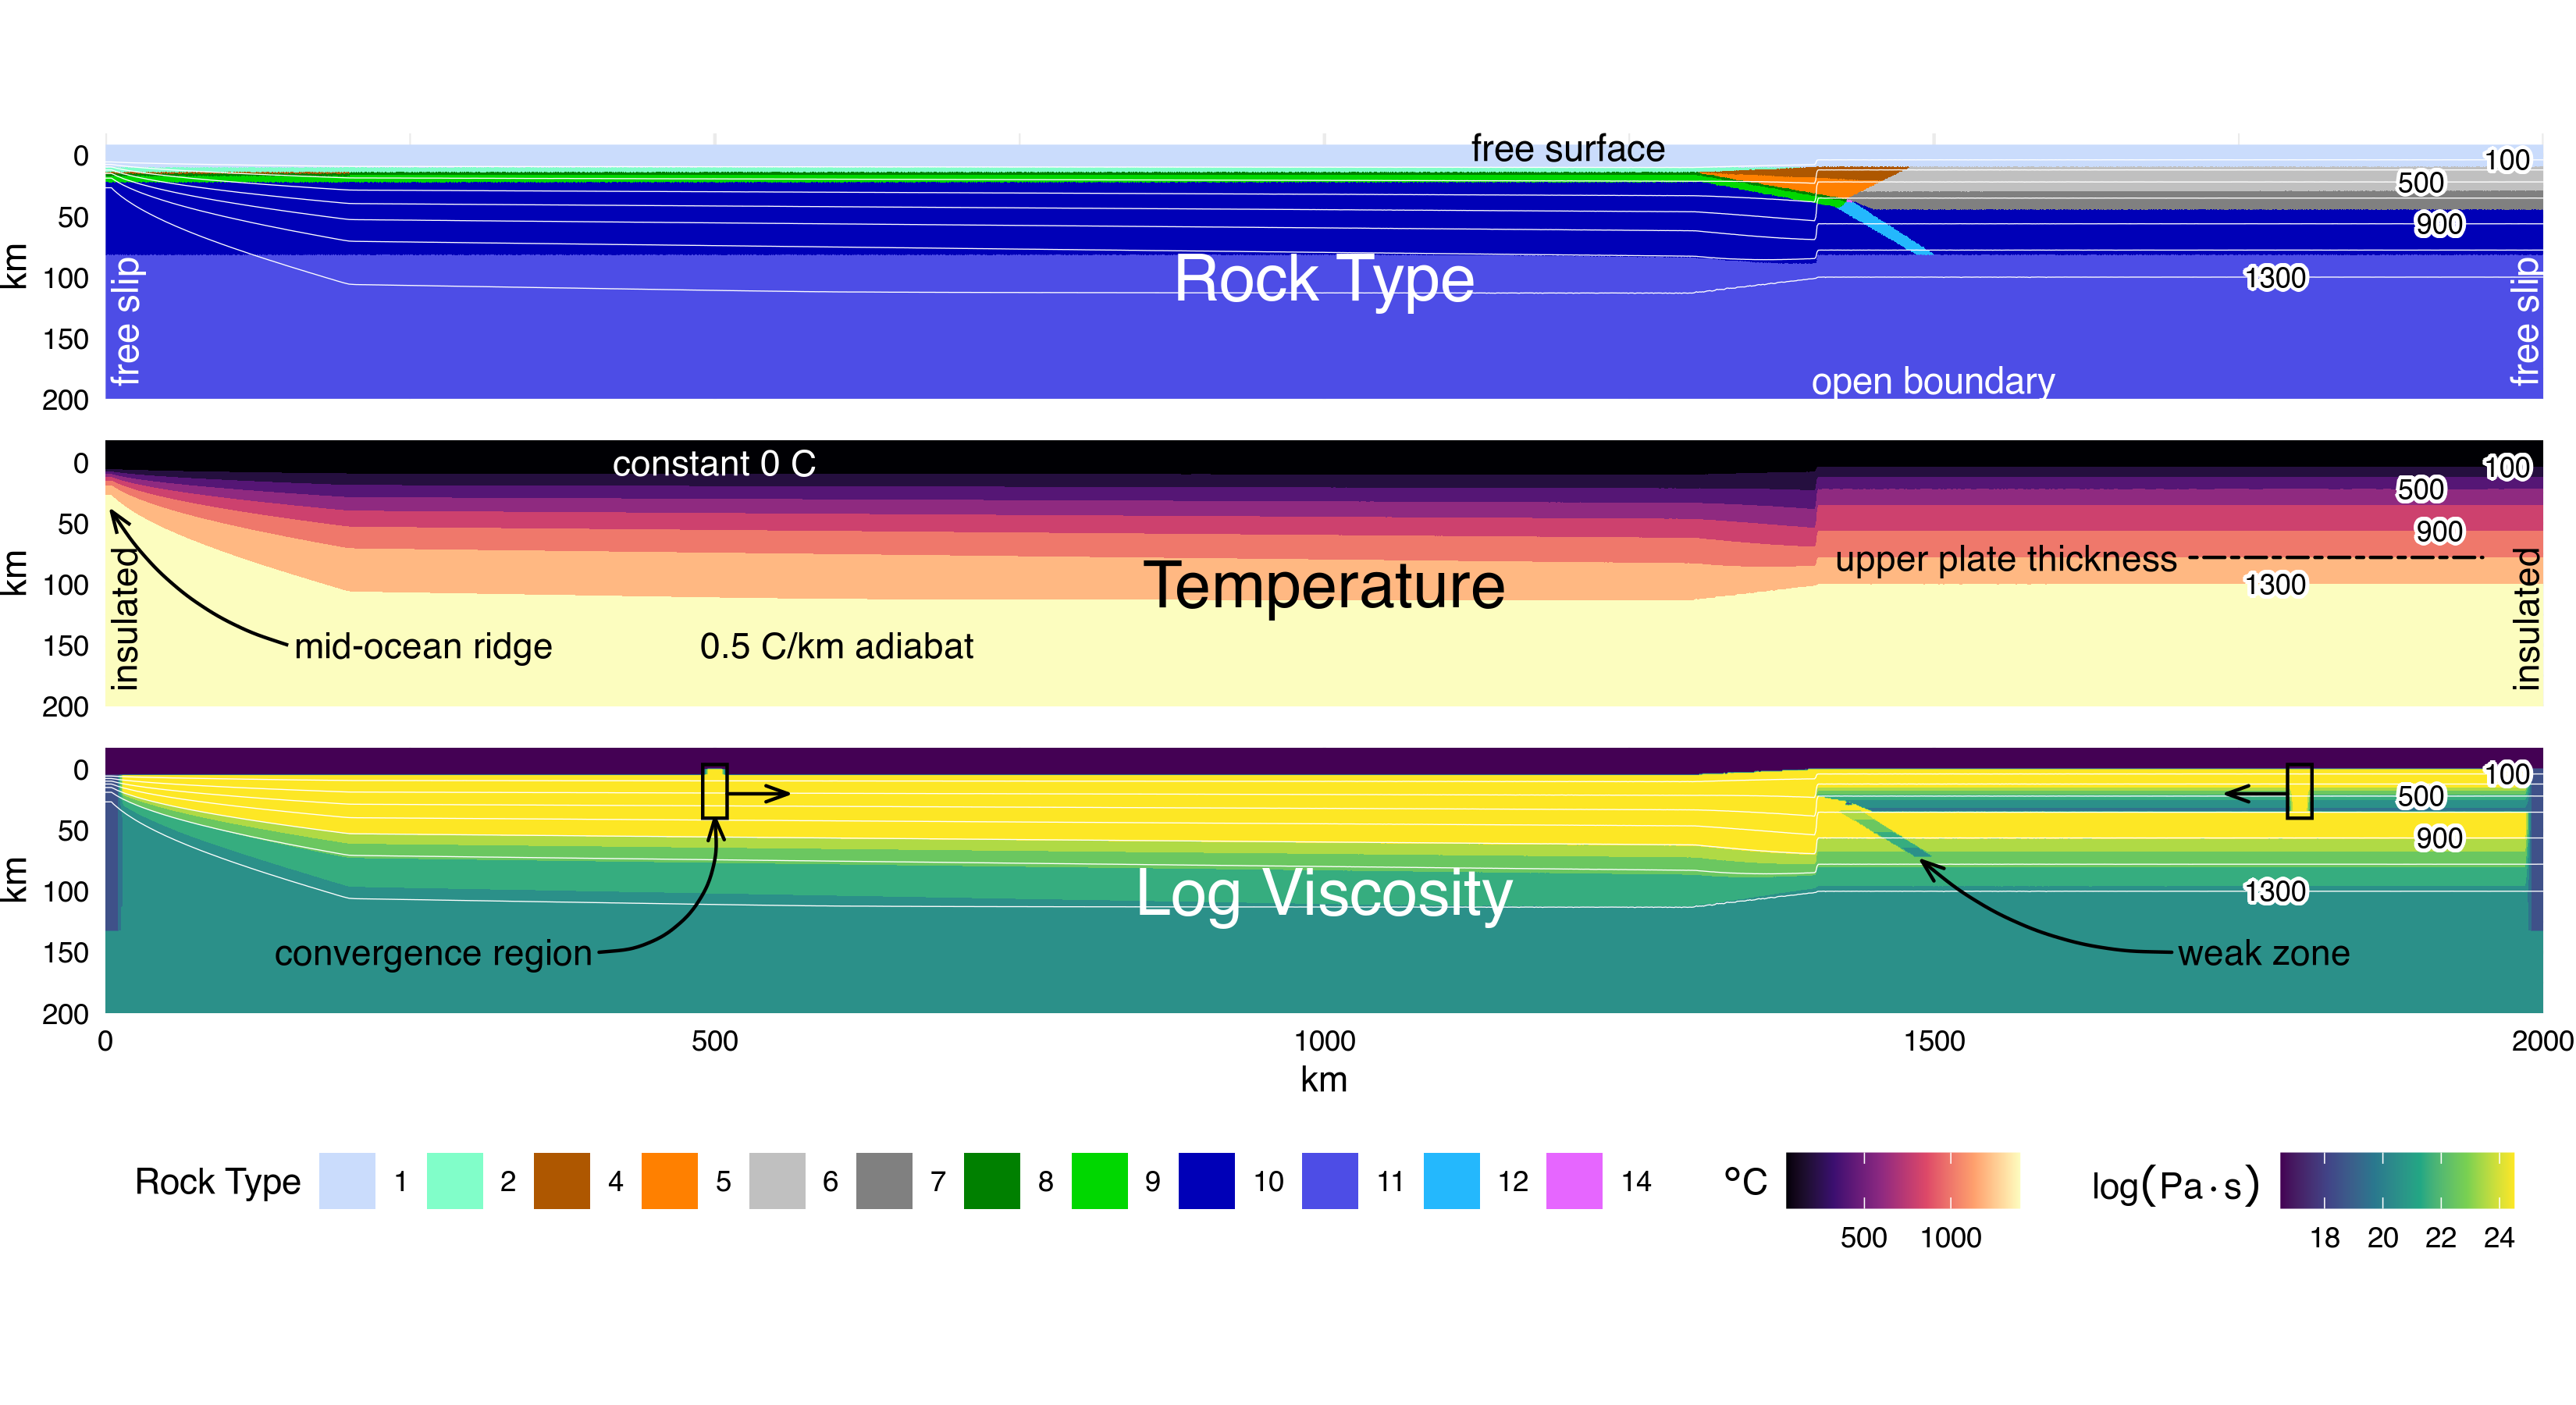
\includegraphics[width=1\linewidth,]{assets/figs/chpt2/fig1} 

}

\caption[Initial model configuration and boundary conditions]{Initial model configuration and boundary conditions. (a) A free sedimentation/erosion boundary at the surface is maintained by implementing a layer of "sticky" air and water, and an infinite-like open boundary at the bottom allows for spontaneous oceanic-plate descent and subduction angle. Left and right boundaries are free slip and thermally insulating. Initial material distribution includes 7 $km$ of oceanic crust (2 $km$ basalt, 5 $km$ gabbro), 1 $km$ of oceanic sediments, and 35 $km$ of continental crust, thinning ocean-ward. (b) Oceanic lithosphere is continually created at the left boundary. The oceanic geotherm is calculated using a half-space cooling model and the continental geotherm is calculated using a one-dimensional steady-state conductive cooling model to 1300 $^{\circ}C$. The base of the upper plate lithosphere ($Z_{UP}$) is defined by visualizing viscosity and generally coincides with the 1100 $^{\circ}C$ isotherm. (c) Oceanic crust is bent under loading from passive margin sediments, and a weak zone extends through the lithosphere to help induce subduction. Convergence velocities are imposed at stationary, high-viscosity regions far from the trench. Rock type colors are: [1] air, [2] water, [4,5] sediments, [6,7] felsic crust, [8] basalt, [9] gabbro, [10,11] dry mantle, [12] hydrated mantle, [14] serpentinized mantle.}\label{fig:init}
\end{figure}

\end{landscape}

\hypertarget{numBCs}{%
\subsection{Initial setup and boundary conditions}\label{numBCs}}

Simulations are 2000 \(km\) wide and 300 \(km\) deep (Figure \ref{fig:init}). In the model domain, three governing equations of heat transport, momentum, and continuity are discretized and solved with a conservative finite-difference marker-in-cell approach on a fully staggered grid as outlined in Gerya \& Yuen (\protect\hyperlink{ref-gerya2003}{2003}). Numerical resolution is non-uniform with higher resolution (1 \(km\) x 1 \(km\)) in a 600 \(km\) wide area surrounding the contact between the oceanic-plate and continental margin, then gradually changing to lower resolution towards the model boundaries (5 \(km\) x 1 \(km\), x- and z-directions, respectively). The left and right boundaries are free-slip and thermally insulating (Figure \ref{fig:init}a, b). Implementation of ``sticky'' air and water allows for a free topographical surface with a simple linear sedimentation and erosion model. The lower boundary is open to allow for oceanic-plate descent with a spontaneous subduction angle (\protect\hyperlink{ref-burg2005}{Burg \& Gerya, 2005}).

A horizontal convergence force is applied to both plates in a rectangular region far from the continental margin (Figure \ref{fig:init}c). An initial weak layer cutting the lithosphere permits subduction to initiate. The high-viscosity (\(\eta = 10^{25}~Pa\cdot s\)) rectangular convergence regions apply constant horizontal velocities without deforming the lithosphere. Subduction angle is governed by free-motion of the subducting plate. Similarly, subduction velocity varies with time in response to extension or shortening of the overriding plate. \(\Phi\) is thus calculated as the product of the horizontal convergence velocity and the oceanic-plate age (c.f. \protect\hyperlink{ref-mckenzie1969}{McKenzie, 1969}). For convenience and consistency with the literature, this study presents \(\Phi\) in units of \(km\)/100 (Figure \ref{fig:params}a).

\begin{figure}[htbp]

{\centering 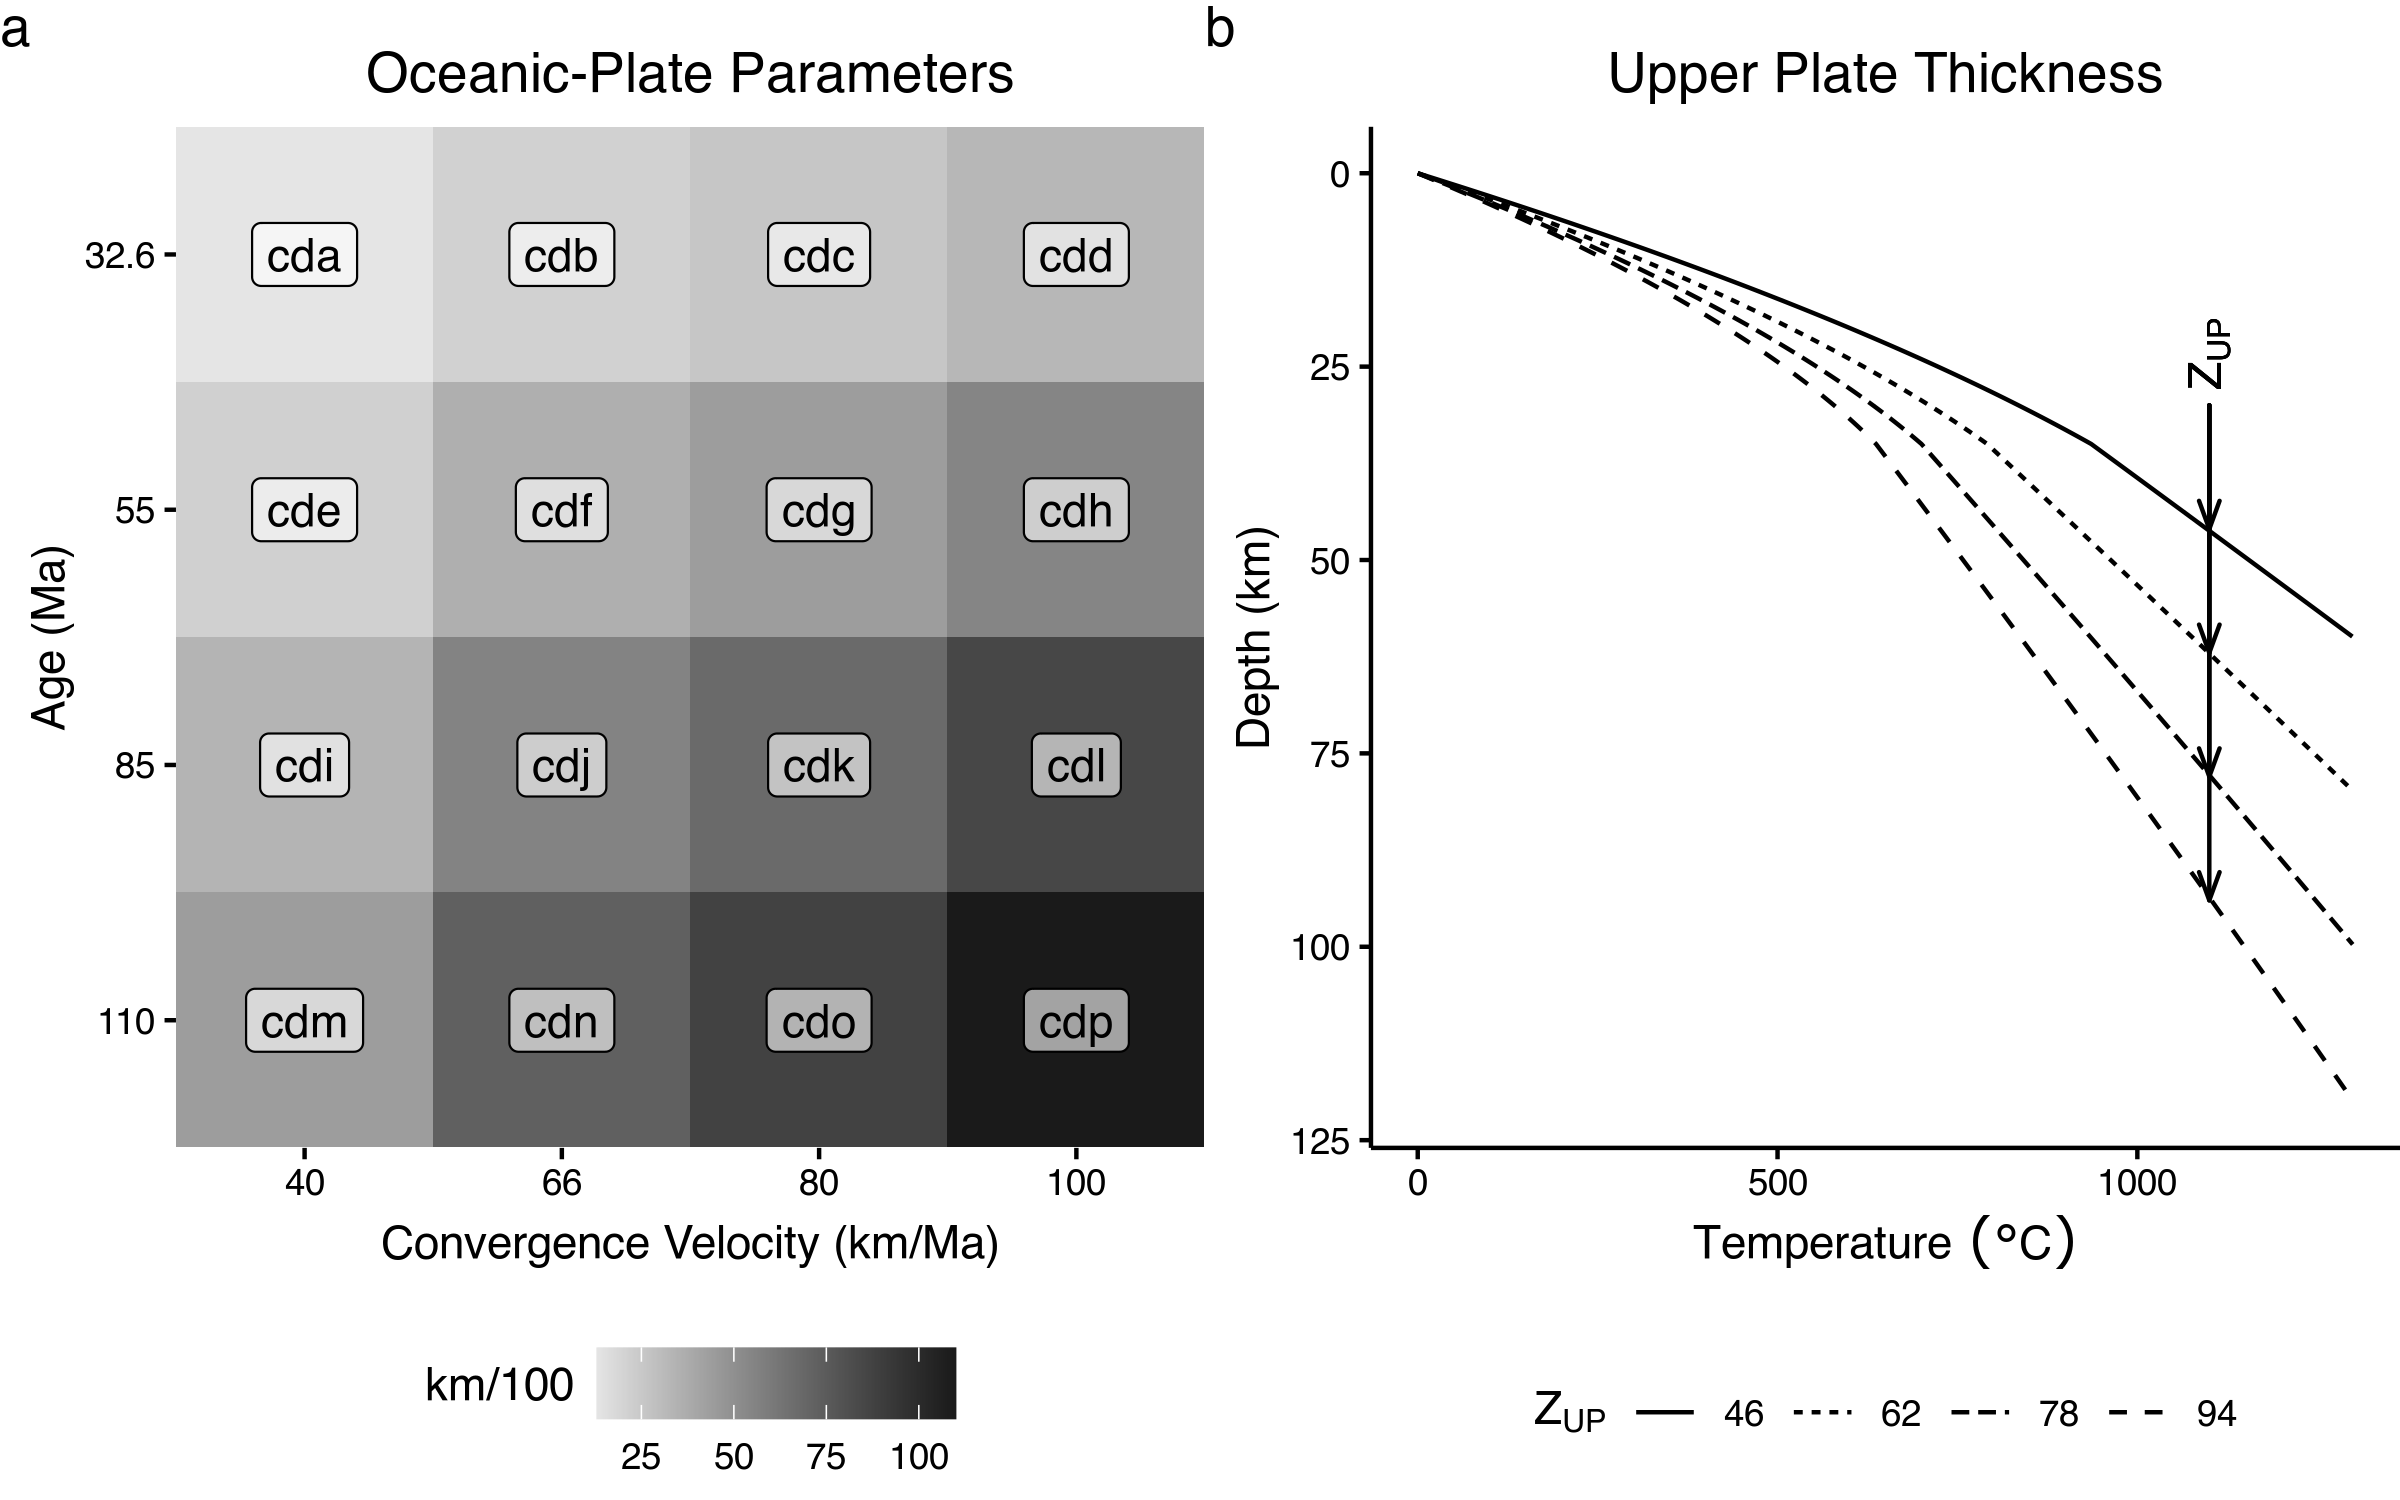
\includegraphics[width=1\linewidth,]{assets/figs/chpt2/fig2} 

}

\caption[Range of boundary conditions used in numerical experiments]{Range of thermo-kinematic boundary conditions used in numerical experiments. (a) Thermal parameters (grayscale) range from 13 to 110 $km/100$ and broadly reflect the distribution of oceanic-plate ages and convergence velocities in modern \glspl{sz}. Model names include the prefix "cd" for "coupling depth" with increasing alphabetic suffixes. Note that neither axes are continuous. (b) Upper plate thickness ($Z_{UP}$) is defined by a range of continental geotherms. Geotherms were constructed using a one-dimensional steady-state conductive cooling model with $T(z=0)$ = 0 $^{\circ}C$, $\vec{q}(z=0)$ = 59, 63, 69, 79 $mW/m^2$, and constant radiogenic heating of 1.0 $\mu W/m^3$ for a 35 $km$-thick crust and 0.022 $\mu W/m^3$ for the mantle. Continental geotherms are calculated up to 1300 $^{\circ}$C with a constant 0.5 $^{\circ}C/km$ gradient (the mantle adiabat) extending to the base of the model domain.}\label{fig:params}
\end{figure}

\hypertarget{numGeotherms}{%
\subsection{Calculating geotherms and defining lithospheric thickness}\label{numGeotherms}}

Oceanic crust is modeled as 1 \(km\) of sediment cover overlying 2 \(km\) of basalt and 5 \(km\) of gabbro (Figure \ref{fig:init}a). Oceanic lithosphere is continually made at a pseudo-mid-ocean ridge at the left boundary of the model (Figure \ref{fig:init}b). An enhanced vertical cooling condition applied at 200 \(km\) from left boundary adjusts for the proper oceanic-plate age, and therefore its lithospheric thickness as it enters the trench (\protect\hyperlink{ref-agrusta2013}{Agrusta et al., 2013}). Oceanic-plate ages range from 32.6 to 110 \(Ma\) and convergence velocities from 40 to 100 \(km/Ma\) (Figure \ref{fig:params}a). This range of parameters broadly reflects the middle-range of modern global subduction systems (\protect\hyperlink{ref-syracuse2006}{Syracuse \& Abers, 2006}).

Initial continental geotherms are determined by solving the heat flow equation in one-dimension to 1300 \(^{\circ}C\) (Figure \ref{fig:params}b). This study assumes a fixed temperature of 0 \(^{\circ}C\) at the surface, constant radiogenic heating of 1 \(\mu W/m^{3}\) in the 35 \(km\)-thick continental crust, 0.022 \(\mu W/m^{3}\) in the mantle, with thermal conductivities of 2.3 \(W/mK\) and 3.0 \(W/mK\) for the continental crust and mantle, respectively. Above, 1300 \(^{\circ}C\), temperature is assumed to constantly increase by 0.5 \(^{\circ}C/km\) (the mantle adiabat) to the base of the model domain.

Many studies define the base of the continental lithosphere at the 1300 \(^{\circ}C\) isotherm, but it can be determined directly by visualizing viscosity and strain rate as the model progresses. The mechanical base of the lithosphere (\(Z_{UP}\)) in the models generally occurs near the 1100 \(^{\circ}C\) isotherm---characterized by a rapid decrease in viscosity and increase in strain rate (Figures \ref{fig:cdfStep1}, \ref{fig:cdfStep2}, \ref{fig:cdfStep3}). As such, this study considers oceanic and continental lithospheres as mechanical layers defined by viscosity, rather than defined merely by temperature. \(Z_{UP}\) corresponding to backarc surface heat flow of 59, 63, 69, and 79 \(mW/m^{2}\) are used in this study (Figure \ref{fig:params}b).

\hypertarget{numHydration}{%
\subsection{Metamorphic (de)hydration reactions}\label{numHydration}}

Using Lagrangian markers (\protect\hyperlink{ref-harlow1962}{Harlow, 1962}, \protect\hyperlink{ref-harlow1964}{1964}) to store and update material properties and \gls{pts} fields allows for straight-forward numerical implementation of metamorphic reactions. This approach is key to regulating mechanical coupling dynamically in \gls{sz} simulations. For example, dehydration (eclogitization) of the oceanic-plate and (de)stabilization of serpentine in the upper-plate mantle may be effectively modelled by tracing marker \gls{ptt} paths while changing marker properties according to thermodynamically-stable mineral assemblages (e.g., \protect\hyperlink{ref-connolly2005}{Connolly, 2005}). For computational efficiency, however, water contents in this study are not computed by iteratively solving thermodynamic systems of equations. Instead, gradual eclogitization of oceanic crust is computed as a linear function of lithostatic pressure to a maximum depth of 150 \(km\), or temperature of 1427 \(^\circ C\), while including garnet-in and plagioclase-out reactions defined by Ito \& Kennedy (\protect\hyperlink{ref-ito1971}{1971}). Mantle (de)hydration is computed according reactions boundaries defined by Schmidt \& Poli (\protect\hyperlink{ref-schmidt1998}{1998}) with a maximum water content of 2 \(wt.\%\) (explained below). This approach effectively simulates continuous influx of water to the upper-plate mantle with relatively low computational cost, beginning with compaction and release of connate water at shallow depths, followed by a sequence of reactions consuming major hydrous phases (chlorite, lawsonite, zoisite, chloritoid, talc, amphibole, and phengite) in different parts of the hydrated basaltic crust (\protect\hyperlink{ref-schmidt1998}{Schmidt \& Poli, 1998}; \protect\hyperlink{ref-vankeken2011}{van Keken et al., 2011}).

The extent of metamorphic reaction effects on mechanical coupling, and the exact (de)hydration reaction(s) likely responsible, are unknown. However, formation of brucite and serpentine from dry olivine near the plate interface are inferred to strongly regulate mechanical behaviour (\protect\hyperlink{ref-agard2016}{Agard et al., 2016}; \protect\hyperlink{ref-hyndman2003}{Hyndman \& Peacock, 2003}; \protect\hyperlink{ref-peacock1999a}{Peacock \& Hyndman, 1999}). Brucite notably breaks down at much lower temperatures than serpentine (\protect\hyperlink{ref-schmidt1998}{Schmidt \& Poli, 1998}), so serpentine (de)stabilization arguably represents the key transition from a weak-to-strong upper-plate mantle deep in \glspl{sz}. This study elects an implementation of serpentine (de)hydration for this reason. The reaction is assumed to be abrupt and discontinuous, which is a fine approximation for near-endmember compositions like (Mg-rich) peridotites. The \gls{pt} conditions of the reaction \(antigorite \Leftrightarrow olivine + orthopyroxene + H_{2}O\) were numerically implemented by the following equation (after \protect\hyperlink{ref-schmidt1998}{Schmidt \& Poli, 1998}):

\begin{equation}
  T_{atg-out}(z)=
  \begin{cases}
    751.50+6.008\times10^{-3}z-3.469\times10^{-8}z^2,& \text{for } z < 63000m \\
    1013.2-6.039\times10^{-5}z-4.289\times10{-9}z^2,& \text{for } z>63000m
  \end{cases}
  \label{eq:antstab}
\end{equation}

where \(z\) is the depth of a marker from the surface in meters and \(T\) is temperature in Kelvins. This reaction boundary is consistent to within 25 \(^{\circ}C\) of more recent experiments by Shen et al. (\protect\hyperlink{ref-shen2015}{2015}). Markers with internal temperature exceeding \(T_{atg-out}(z)\) spontaneously form \(olivine + orthopyroxene + H_{2}O\) and release their crystal-bound water. This implementation tacitly assumes thermodynamic equilibrium and is common to many versions of \texttt{I2VIS}.

Oceanic-plates of different ages are also tacitly assumed to dehydrate similarly with the above implementation. However, older (colder) oceanic-plates are expected to carry water to greater depths than younger (warmer) plates because of relatively delayed water-releasing reactions (\protect\hyperlink{ref-peacock1996}{Peacock, 1996}). Abrupt water release with serpentine dehydration (Equation \eqref{eq:antstab}) was tested to model deep water retention in cold oceanic-plates. Mechanical coupling behaviour was indistinguishable from gradual water release models. This implies rates of water release are less important than the depth of serpentine stability. Explicitly modelling other major dehydration reactions are thus unlikely to significantly affect mechanical coupling behaviour, yet likely to introduce numerical artifacts at great computational cost. A simplified gradual water release model for all oceanic-plates is therefore preferred.

Water released by rock forms discrete fluid particles that migrate with relative velocities defined by local deviatoric (non-lithostatic) pressure gradients (see Appendix \ref{deHydration}, \protect\hyperlink{ref-faccenda2009}{Faccenda et al., 2009}). Fluid velocities are scaled by a 10 \(cm/yr\) vertical percolation velocity to account for purely lithostatic pressure gradients in the mantle (\protect\hyperlink{ref-gorczyk2007}{Gorczyk et al., 2007}). Fluid particles migrate until encountering rock that can consume additional water by equilibrium hydration or melting reactions, (Equation \ref{tab:melts}).

The shallow upper-plate mantle can theoretically store large amounts of water as serpentine may contain up to 13 \(wt.\%\) water (\protect\hyperlink{ref-reynard2013}{Reynard, 2013}) and is generally stable at shallow mantle conditions. Thermodynamic models predict 8 \(wt.\%\) water in the shallow upper-plate mantle (\protect\hyperlink{ref-connolly2005}{Connolly, 2005}). However, seismic studies suggest most shallow upper-plate mantles are only partially serpentinized (\textless{} 20-40\%), equating to water contents of approximately 3-6 \(wt.\%\) (\protect\hyperlink{ref-abers2017}{Abers et al., 2017}; \protect\hyperlink{ref-carlson2003}{Carlson \& Miller, 2003}). Many modes of mantle hydration are documented or inferred, including evidence for channelized fluid flow within ophiolites exhumed from \glspl{sz} (\protect\hyperlink{ref-angiboust2012a}{Angiboust et al., 2012}, \protect\hyperlink{ref-angiboust2014}{2014}; \protect\hyperlink{ref-plumper2017}{Plümper et al., 2017}; \protect\hyperlink{ref-zack2007}{Zack \& John, 2007}). This study limits mantle wedge hydration to \(\leq\) 2 \(wt.\%~H_{2}O\) and assumes any excess \(H_{2}O\) exits the system through channelized fluid flow during plastic or brittle deformation (\protect\hyperlink{ref-davies1999}{Davies, 1999}).

\begin{table}

\caption{\label{tab:materials}Material properties used in numerical experiments}
\centering
\resizebox{\linewidth}{!}{
\begin{threeparttable}
\begin{tabular}[t]{lrrlrrrrrrrrlr}
\toprule
Material & $\rho$ & $H_2O$ & Flow Law & $log_{10}A$ & $E$ & $V$ & $n$ & $\phi$ & $\sigma_{crit}$ & $k_1$ & $k_2$ & $k_3$ & $H$\\
\midrule
\cellcolor{gray!6}{sediments} & \cellcolor{gray!6}{2600} & \cellcolor{gray!6}{5.0} & \cellcolor{gray!6}{wet quartzite} & \cellcolor{gray!6}{-3.5} & \cellcolor{gray!6}{154.0} & \cellcolor{gray!6}{3.0} & \cellcolor{gray!6}{2.3} & \cellcolor{gray!6}{0.15} & \cellcolor{gray!6}{0.03} & \cellcolor{gray!6}{0.64} & \cellcolor{gray!6}{807} & \cellcolor{gray!6}{4e-06} & \cellcolor{gray!6}{2.000}\\
felsic crust & 2700 &  & wet quartzite & -3.5 & 154.0 & 3.0 & 2.3 & 0.45 & 0.03 & 0.64 & 807 & 4e-06 & 1.000\\
\cellcolor{gray!6}{basalt} & \cellcolor{gray!6}{3000} & \cellcolor{gray!6}{5.0} & \cellcolor{gray!6}{plag an75} & \cellcolor{gray!6}{-3.5} & \cellcolor{gray!6}{238.0} & \cellcolor{gray!6}{8.0} & \cellcolor{gray!6}{3.2} & \cellcolor{gray!6}{0.45} & \cellcolor{gray!6}{0.03} & \cellcolor{gray!6}{1.18} & \cellcolor{gray!6}{474} & \cellcolor{gray!6}{4e-06} & \cellcolor{gray!6}{0.250}\\
gabbro & 3000 &  & plag an75 & -3.5 & 238.0 & 8.0 & 3.2 & 0.45 & 0.03 & 1.18 & 474 & 4e-06 & 0.250\\
\cellcolor{gray!6}{mantle dry} & \cellcolor{gray!6}{3300} & \cellcolor{gray!6}{} & \cellcolor{gray!6}{dry olivine} & \cellcolor{gray!6}{4.4} & \cellcolor{gray!6}{540.0} & \cellcolor{gray!6}{20.0} & \cellcolor{gray!6}{3.5} & \cellcolor{gray!6}{0.45} & \cellcolor{gray!6}{0.30} & \cellcolor{gray!6}{0.73} & \cellcolor{gray!6}{1293} & \cellcolor{gray!6}{4e-06} & \cellcolor{gray!6}{0.022}\\
\addlinespace
mantle hydrated & 3300 & 0.5 & wet olivine & 3.3 & 430.0 & 10.0 & 3.0 & 0.45 & 0.24 & 0.73 & 1293 & 4e-06 & 0.022\\
\cellcolor{gray!6}{serpentine} & \cellcolor{gray!6}{3200} & \cellcolor{gray!6}{2.0} & \cellcolor{gray!6}{serpentine} & \cellcolor{gray!6}{3.3} & \cellcolor{gray!6}{8.9} & \cellcolor{gray!6}{3.2} & \cellcolor{gray!6}{3.8} & \cellcolor{gray!6}{0.15} & \cellcolor{gray!6}{3.00} & \cellcolor{gray!6}{0.73} & \cellcolor{gray!6}{1293} & \cellcolor{gray!6}{4e-06} & \cellcolor{gray!6}{0.022}\\
\bottomrule
\end{tabular}
\begin{tablenotes}
\item \uline{\textit{key}}: $\rho$: density $[kg/m^3]$, $H_2O$: water content $[wt.\%]$, $A$: material constant, $E$: activation energy $[kJ/mol]$, $V$: activation volume $[J/MPa\cdot mol]$, $n$: power law exponent, $\phi$: internal friction angle, $\sigma_{crit}$: critical stress $[MPa]$, $H$: heat production $[\mu W/m^3]$
\item \uline{\textit{constants}}: $C_p$: heat capacity = $1~[kJ/kg]$, $\alpha$: expansivity = $2\times 10^{-5}~[1/K]$, $\beta$: compressibility = $0.045~[1/MPa]$
\item \uline{\textit{thermal conductivity}}: $k$ $[W/m \cdot K]=(k_1+\frac{k_2}{T+77})\times exp(k_3 \cdot P)$ with $P$ in $[MPa]$ and $T$ in $[K]$
\item \uline{\textit{references}}: Turcotte \& Schubert (2002), Ranalli (1995), Hilairet et al. (2007), Karato \& Wu (1993)
\end{tablenotes}
\end{threeparttable}}
\end{table}

\hypertarget{rheologicModel}{%
\subsection{Rheologic model}\label{rheologicModel}}

Contributions from dislocation and diffusion creep are accounted for by computing a composite rheology for ductile rocks, \(\eta_{effective}\):

\begin{equation}
  \begin{aligned}
    \frac{1}{\eta_{effective}} = \frac{1}{\eta_{diff}} + \frac{1}{\eta_{disl}}
  \end{aligned} 
  \label{eq:ductile}
\end{equation}

where \(\eta_{diff}\) and \(\eta_{disl}\) are effective viscosities for diffusion and dislocation creep.

For the crust and serpentinized mantle, \(\eta_{diff}\) and \(\eta_{disl}\) are computed as:

\begin{equation}
  \begin{aligned}
    \eta_{diff} &= \frac{1}{2} \ A \ \sigma_{crit}^{1-n} \ \exp\left[\frac{E+PV}{RT}\right] \\
    \eta_{disl} &= \frac{1}{2} \ A^{1/n} \ \dot{\varepsilon}_{II}^{(1-n)/n} \ \exp\left[\frac{E+PV}{nRT}\right]
  \label{eq:crust}
  \end{aligned}
\end{equation}

where \(R\) is the gas constant, \(P\) is pressure, \(T\) is temperature in \(K\), \({\dot{\varepsilon}}_{II} = \sqrt{\frac{1}{2}{{\dot{\varepsilon}}_{ij}}^{2}}\) is the square root of the second invariant of the strain rate tensor, \(\sigma_{crit}\) is an assumed diffusion-dislocation transition stress, and \(A\), \(E\), \(V\) and \(n\) are the material constant, activation energy, activation volume, and stress exponent, respectively (Table \ref{tab:materials}, \protect\hyperlink{ref-hilairet2007}{Hilairet et al., 2007}; \protect\hyperlink{ref-ranalli1995}{Ranalli, 1995}).

For the mantle, \(\eta_{diff}\) and \(\eta_{disl}\) are computed as (\protect\hyperlink{ref-karato1993}{Karato \& Wu, 1993}):

\begin{equation}
  \begin{aligned}
    \eta_{diff} &= \frac{1}{2} \ A^{-1} \ G \ \left[\frac{h}{b}\right]^{m/n} \ \exp\left[\frac{E+PV}{RT}\right] \\
    \eta_{disl} &= \frac{1}{2} \ A^{-1/n} \ G \ \dot{\varepsilon}_{II}^{(1-n)/n} \ \exp\left[\frac{E+PV}{nRT}\right]
  \end{aligned}
  \label{eq:mantle}
\end{equation}

where \(b\)=\(5\times10^{-10}\) \(m\) is Burgers vector, \(G\)=\(8\times10^{10}\) \(Pa\) is shear modulus, \(h\)=\(1\times10^{-3}\) \(m\) is the assumed grain size, \(m=2.5\) is the grain size exponent, and the other flow law parameters are given in Table \ref{tab:materials}. Our models limited viscosity for all rocks at \(\eta_{min} = 10^{17}\ Pa \cdot s\) and \(\eta_{max} = 10^{25}\ Pa \cdot s\).

An effective visco-plastic rheology is achieved by limiting \(\eta_{effective}\) with a brittle (plastic) yield criterion:

\begin{equation}
  \eta_{effective} \leq \frac{C + \phi \ P}{2 \ \dot{\varepsilon}_{II}}
  \label{eq:plastic}
\end{equation}

where \(\phi\) is the internal friction coefficient, \(C\) cohesive strength at \(P\) = 0, and \({\dot{\varepsilon}}_{ij}\) is the strain rate tensor (Table \ref{tab:materials}).

\hypertarget{visualization-and-determination-of-coupling-depth}{%
\subsection{Visualization and determination of coupling depth}\label{visualization-and-determination-of-coupling-depth}}

The rheologic model and \gls{tkbc} described in the previous sections always results in plate motions towards the left boundary (slab-rollback). Relatively high dip angles and extreme subduction velocities in some high-\(\Phi\) experiments cause chaotic behaviour by 10 \(Ma\) as the upper-plate is stretched thin and mechanical interference occurs between trench sediments and the high-viscosity convergence region 200 \(km\) from the left boundary. Numerical solutions are stable for most experiments, however, reaching quasi-steady state by 5 \(Ma\). An additional 5 \(Ma\) is allowed to ensure stable geodynamics before observing \gls{cd}. Surface heat flow, rock type, temperature, viscosity, strain rate, shear heating, and velocity fields are visualized at approximately 10 \(Ma\) (e.g., Figure \ref{fig:comp}) for all 64 experiments to assess geodynamics and solution stability (Figure \ref{fig:antDepth}).

\begin{figure}[htbp]

{\centering 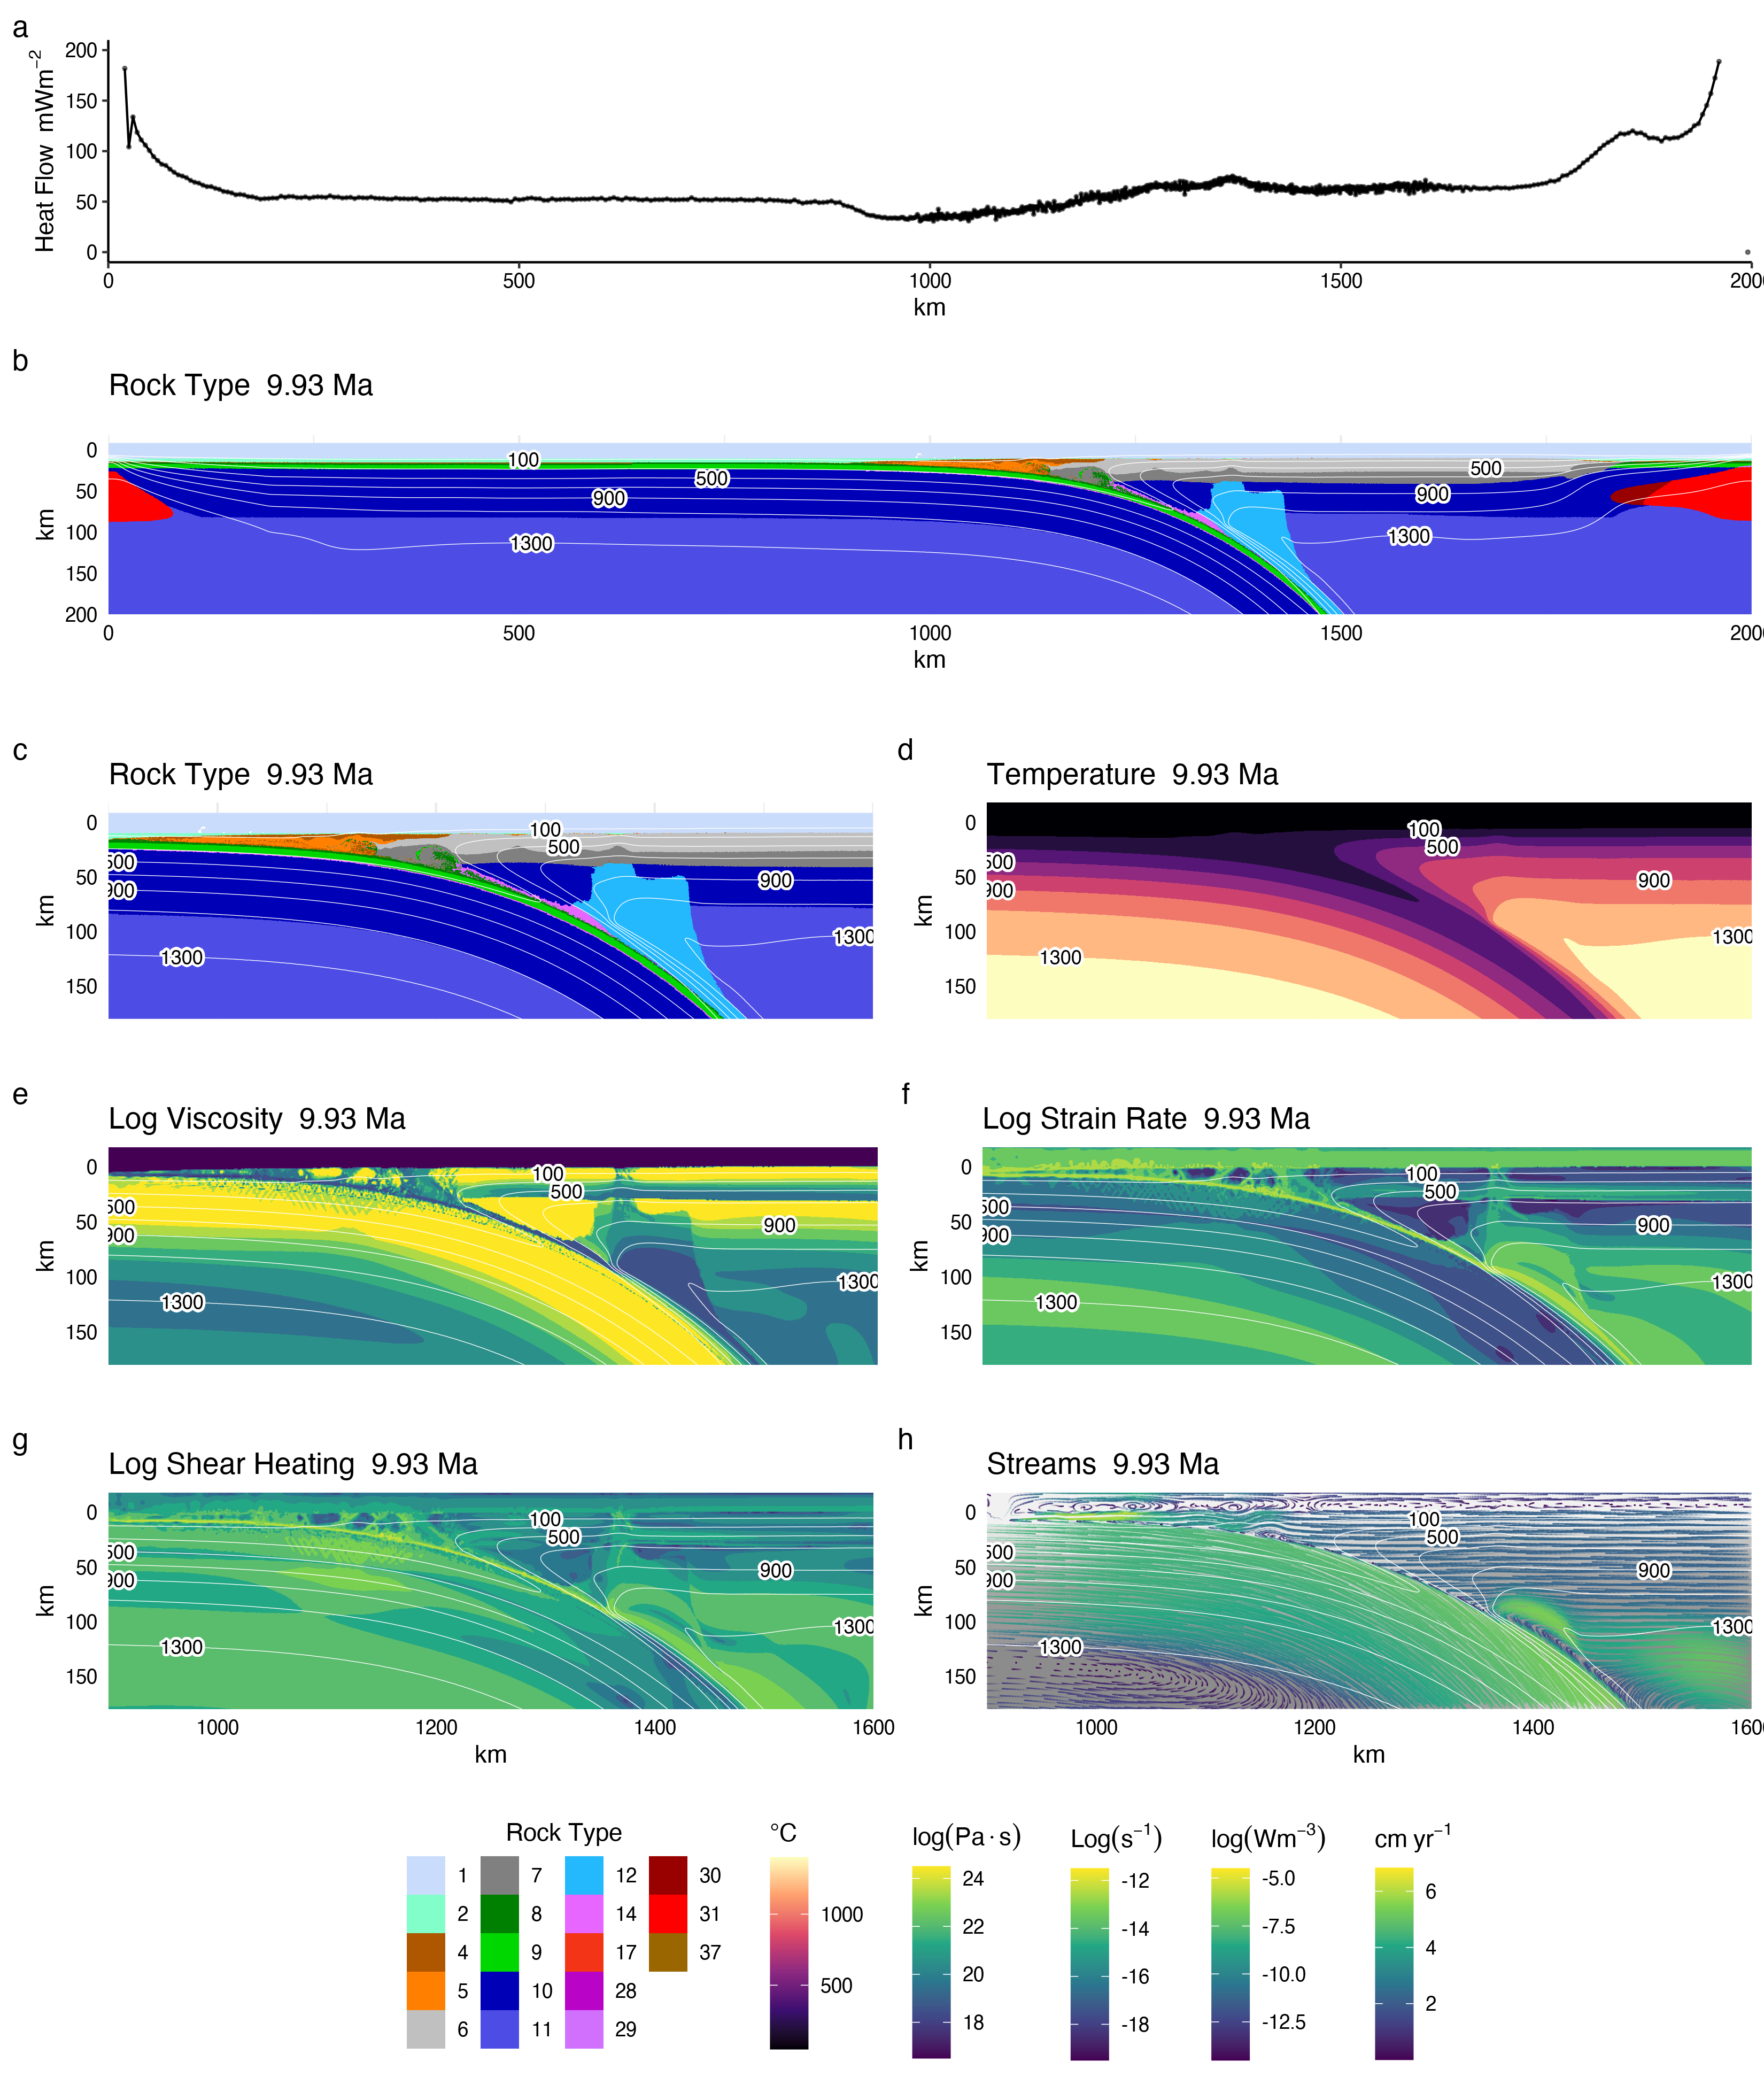
\includegraphics[width=1\linewidth,]{assets/figs/chpt2/fig3} 

}

\caption[Numerical experiment visualization]{Visualizing model cdf with a 78 $km$ upper-plate lithosphere at approximately 10 $Ma$. (a) Rock type shows a thin serpentine layer (pink) lubricating the plate interface. Note that low melt volumes are inconspicuous and quickly extracted. (b) Viscosity shows high contrast between the oceanic-plate and serpentinized upper-plate mantle at shallow levels. Viscosity contrast disappears where serpentine becomes unstable. (c) Streamlines show focused mantle flow towards the interface, coinciding with the lower limit of serpentine stability. Note the converging isotherms that imply a feedback between heat transfer, serpentine destabilization, and mechanical coupling. (d) Strain rate shows localized deformation in the serpentine layer along the plate interface. Note that deformation in the upper-plate mantle is restricted to viscous flow beneath the lithosphere and along narrow, subvertical melt conduits. Rock type colors are the same as Figure 1.}\label{fig:comp}
\end{figure}

After approximately 10 \(Ma\) of subduction \gls{cd} is determined directly from viscosity by finding the approximate area where strength contrasts between serpentinized- and non-serpentinized upper-plate mantle diminishes to \(<\) 10\(^2\) \(Pa \cdot s\). The node nearest to this region is assigned as the \gls{cd}. This study assumes mechanical coupling occurs instantaneously and at a single node. Mechanical coupling in reality must be dispersed across a finite length along the plate interface, however. At the numerical resolution the experiments, coupling-like viscosity contrasts are similar within a small area (approximately 5 \(\times\) 5 \(km\) or 5 \(\times\) 5 nodes), giving a qualitative uncertainty \gls{cd} on the order of 2.5 \(km\).

\hypertarget{chpt2Results}{%
\section{Results}\label{chpt2Results}}

\hypertarget{cdEstimators}{%
\subsection{Coupling depth estimators}\label{cdEstimators}}

\gls{cd} (\(Z_{cpl}\)) correlates strongly with \gls{upt} (\(Z_{UP}\)) and weakly with \(\Phi\) across all 64 numerical models (Table \ref{tab:zcResults}, Figures \ref{fig:results} \& \ref{fig:biv}). The responsiveness of \gls{cd} to \(Z_{UP}\) but not to \(\Phi\) is a key result of our experiments. The following equation minimizes standard least squares while optimizing the number of parameters, \emph{p value}, and \(R^2\) for all possible permutations of the variables \(Z_{UP}\) and \(\Phi\) in linear and quadratic forms:

\begin{equation}
  Z_{cpl} = 4.95\times 10^{-3}\ Z_{UP}^{2}\ -\ 9.27\times 10^{-2}\ \Phi\ +\ 63.6
  \label{eq:zCpl}
\end{equation}

where \(Z_{cpl}\) is coupling depth in \(km\) and \(\Phi\) is the thermal parameter in \(km/100\). Regression summaries show both linear and quadratic models of \(Z_{cpl}\) vs.~\(Z_{UP}\) and \(\Phi\) fit experimental results well (Tables \ref{tab:anova} \& \ref{tab:regSummary}). Equation \eqref{eq:zCpl} represents a statistical model formulated with observations from physics-based simulations of subduction. Equation \eqref{eq:zCpl} is useful for estimating \glspl{cd} in active \glspl{sz} where \(\Phi\) is known and \(Z_{UP}\) can be inverted from \gls{shf}.

\begin{table}

\caption{\label{tab:segs}Estimated coupling depths for active subduction zones}
\centering
\begin{threeparttable}
\begin{tabular}[t]{lrrrrrr}
\toprule
Segment & $\vec{q}$ & $Z_{UP}$ & $\Phi$ & $Z_{cpl}^a$ & $Z_{cpl}^b$ & $Z_{cpl}^c$\\
\midrule
\cellcolor{gray!6}{N. Cascadia} & \cellcolor{gray!6}{75} & \cellcolor{gray!6}{74.2} & \cellcolor{gray!6}{3.4} & \cellcolor{gray!6}{92} & \cellcolor{gray!6}{91} & \cellcolor{gray!6}{90}\\
Nankai & 69 & 96.3 & 6.9 & 107 & 109 & 110\\
\cellcolor{gray!6}{Mexico} & \cellcolor{gray!6}{72} & \cellcolor{gray!6}{98.1} & \cellcolor{gray!6}{7.2} & \cellcolor{gray!6}{108} & \cellcolor{gray!6}{111} & \cellcolor{gray!6}{112}\\
Columbia-Ecuador & 80 & 66.4 & 10.4 & 86 & 84 & 84\\
\cellcolor{gray!6}{S.C. Chile} & \cellcolor{gray!6}{80} & \cellcolor{gray!6}{66.4} & \cellcolor{gray!6}{20.0} & \cellcolor{gray!6}{85} & \cellcolor{gray!6}{84} & \cellcolor{gray!6}{83}\\
\addlinespace
Kyushu & 69 & 83.2 & 13.5 & 97 & 97 & 96\\
\cellcolor{gray!6}{N. Sumatra} & \cellcolor{gray!6}{120} & \cellcolor{gray!6}{26.8} & \cellcolor{gray!6}{25.0} & \cellcolor{gray!6}{57} & \cellcolor{gray!6}{65} & \cellcolor{gray!6}{68}\\
Alaska & 80 & 66.4 & 25.3 & 85 & 83 & 82\\
\cellcolor{gray!6}{N. Chile} & \cellcolor{gray!6}{85} & \cellcolor{gray!6}{58.7} & \cellcolor{gray!6}{38.4} & \cellcolor{gray!6}{78} & \cellcolor{gray!6}{77} & \cellcolor{gray!6}{77}\\
N. Costa Rica & 80 & 58.5 & 20.4 & 80 & 79 & 78\\
\addlinespace
\cellcolor{gray!6}{Aleutians} & \cellcolor{gray!6}{75} & \cellcolor{gray!6}{51.6} & \cellcolor{gray!6}{39.6} & \cellcolor{gray!6}{73} & \cellcolor{gray!6}{73} & \cellcolor{gray!6}{73}\\
N. Hikurangi & 80 & 58.5 & 41.0 & 78 & 77 & 76\\
\cellcolor{gray!6}{Mariana} & \cellcolor{gray!6}{80} & \cellcolor{gray!6}{47.5} & \cellcolor{gray!6}{54.6} & \cellcolor{gray!6}{69} & \cellcolor{gray!6}{70} & \cellcolor{gray!6}{70}\\
Kermadec & 80 & 47.5 & 60.0 & 68 & 69 & 70\\
\cellcolor{gray!6}{Kamchatka} & \cellcolor{gray!6}{70} & \cellcolor{gray!6}{80.2} & \cellcolor{gray!6}{77.0} & \cellcolor{gray!6}{89} & \cellcolor{gray!6}{88} & \cellcolor{gray!6}{88}\\
\addlinespace
Izu & 80 & 47.5 & 77.0 & 67 & 68 & 68\\
\cellcolor{gray!6}{NE Japan} & \cellcolor{gray!6}{88} & \cellcolor{gray!6}{47.7} & \cellcolor{gray!6}{107.9} & \cellcolor{gray!6}{64} & \cellcolor{gray!6}{65} & \cellcolor{gray!6}{65}\\
\bottomrule
\end{tabular}
\begin{tablenotes}
\item \uline{\textit{key}}: $\vec{q}$: average backarc surface heat flow $[mWm^{-2}]$, $Z_{UP}$: upper-pate thickness $[km]$, $\Phi$: thermal parameter = $[km/100]$, $Z_{cpl}$: coupling depth $[km]$
\item \uline{\textit{estimators}}: a: $[Z_{cpl}=Z_{UP}+\Phi]$, b: $[Z_{cpl}=Z_{UP}^2+\Phi]$, c: $[Z_{cpl}=Z_{UP}+Z_{UP}^2+\Phi]$
\item \uline{\textit{references}}: Currie \& Hyndman (2006), Wada \& Wang (2009)
\end{tablenotes}
\end{threeparttable}
\end{table}

Sensitivity of \gls{cd} to \gls{upt} and \(\Phi\) is apparent when visualizing Equation \eqref{eq:zCpl} and other regression models across \(Z_{UP}\) and \(\Phi\) space \ref{fig:multiv}. Applying Equation \eqref{eq:zCpl} to 17 active \gls{sz} segments (Table \ref{tab:segs}) gives a wide range of estimated \glspl{cd}, similar to our model simulations. The distribution of estimated \glspl{cd}, however, is relatively narrow and quasi-normal, with a mean of \(\sim\) 82 \(km\) and standard deviation of 7 \(km\) (Figure \ref{fig:multiv}d).

\begin{figure}[htbp]

{\centering 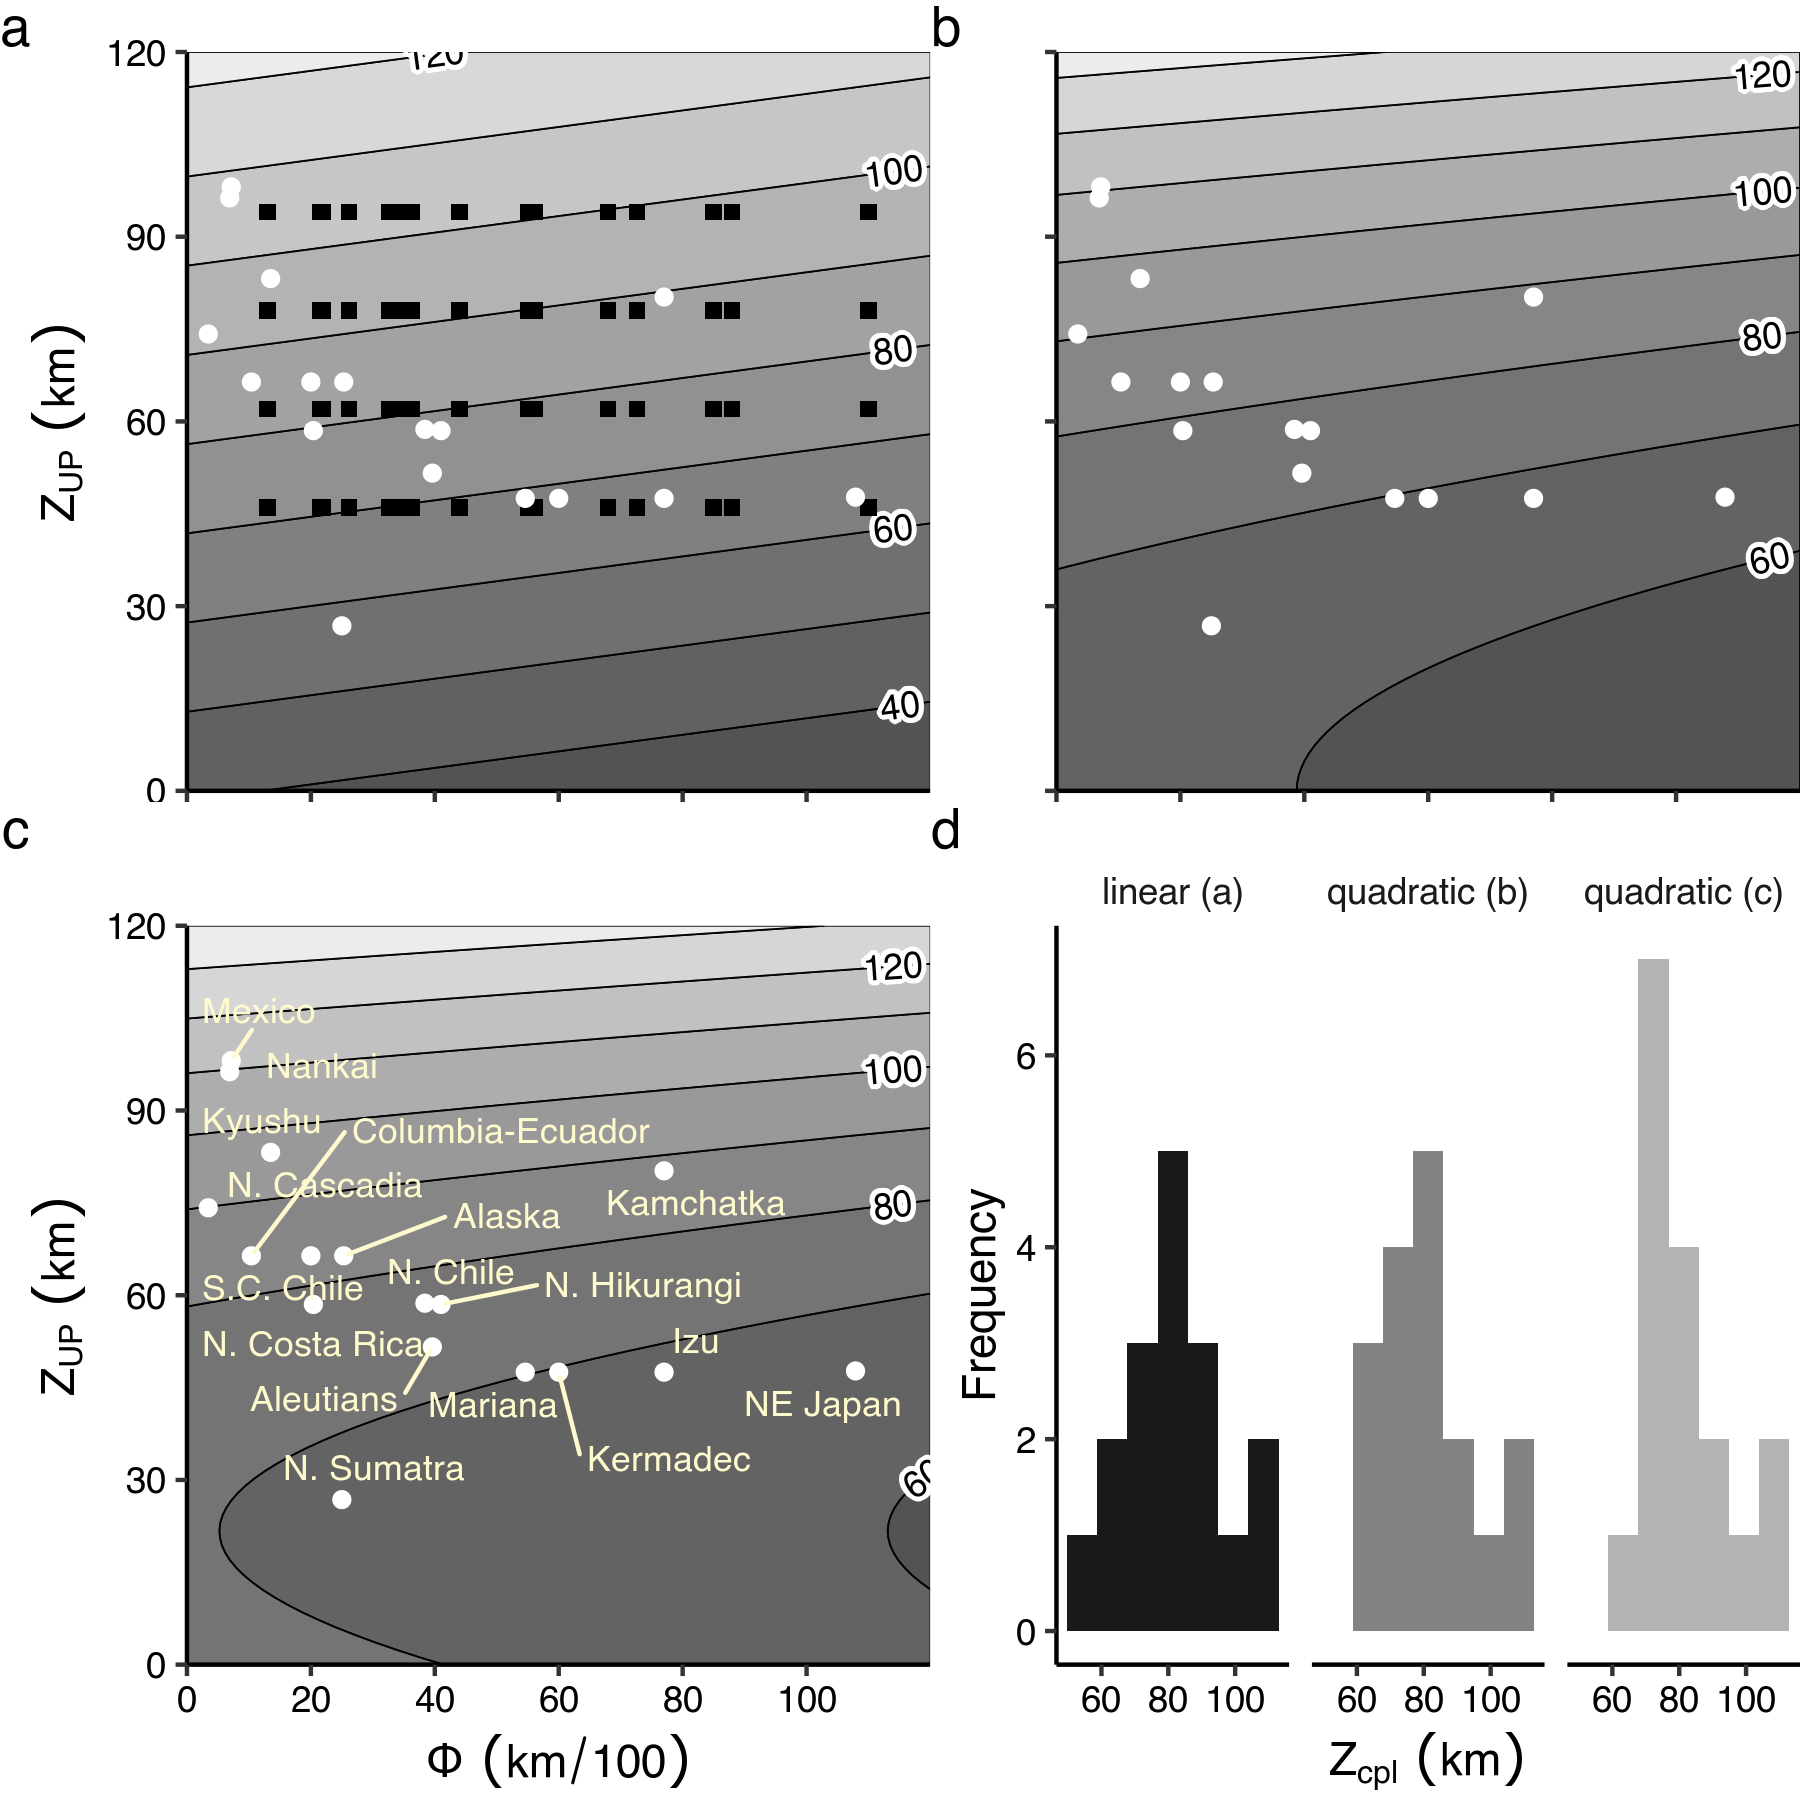
\includegraphics[width=1\linewidth,]{assets/figs/chpt2/fig4} 

}

\caption[Estimated coupling depths for 17 active \gls{sz} segments]{Multivariate regressions and estimated coupling depth ($Z_{cpl}$) for 17 active \gls{sz} segments. Contoured plots show estimated $Z_{cpl}$ (contours) as a function of thermal parameter ($\Phi$) and upper-plate thickness ($Z_{UP}$) for linear (a) and quadratic (b, c) regressions. The best fit regression is panel b (Equation \ref{eq:zCpl}, see Tables \ref{tab:anova} and \ref{tab:regSummary}). Black squares represent numerical experiments used to fit the contours. White points represent active \glspl{sz} (Table \ref{tab:segs}). Contours imply $Z_{cpl}$ depends strongly on $Z_{UP}$, regardless of the regression equation form. Estimated $Z_{cpl}$ for \glspl{sz} with similar $\Phi$ are quite different (e.g., Alaska vs. N. Sumatra). Estimated $Z_{cpl}$ are also quite similar for \glspl{sz} with very different $\Phi$ (e.g., Kamchatka vs. N. Cascadia). (d) Distributions of estimated $Z_{cpl}$ for 17 active \glspl{sz} shown in (a), (b), and (c). These 17 segments span a large range of $\Phi$ but are expected to have a relatively narrow distribution of $Z_{cpl}$ (82 $\pm$ 14 $km$) according to the regressions in (a), (b), and (c).}\label{fig:multiv}
\end{figure}

\hypertarget{surface-heat-flow}{%
\subsection{Surface heat flow}\label{surface-heat-flow}}

Upper-plate \gls{shf} remains relatively stable and reflects initial upper-plate geotherms in the backarc region for experiments with low to moderate \(\Phi\) (Figure \ref{fig:hf}). However, high-amplitude and high-frequency positive \gls{shf} deviations in the upper-plate are common in all experiments, especially for high-\(\Phi\) experiments. These deviations correspond to extensional deformation and heat transport via lithospheric thinning and melt migration. These features are apparent as subvertical low viscosity, high strain rate columns originating from the plate interface (Figure \ref{fig:comp}b, d) and point to potential sources of error when inverting \gls{shf} in active \glspl{sz}. Notably, the backarc is relatively unaffected by fluid and melt migration compared to the forearc. Estimating \gls{upt} by inverting \gls{shf} in the backarc is therefore preferable to forearc \gls{shf}.

\begin{figure}[htbp]

{\centering 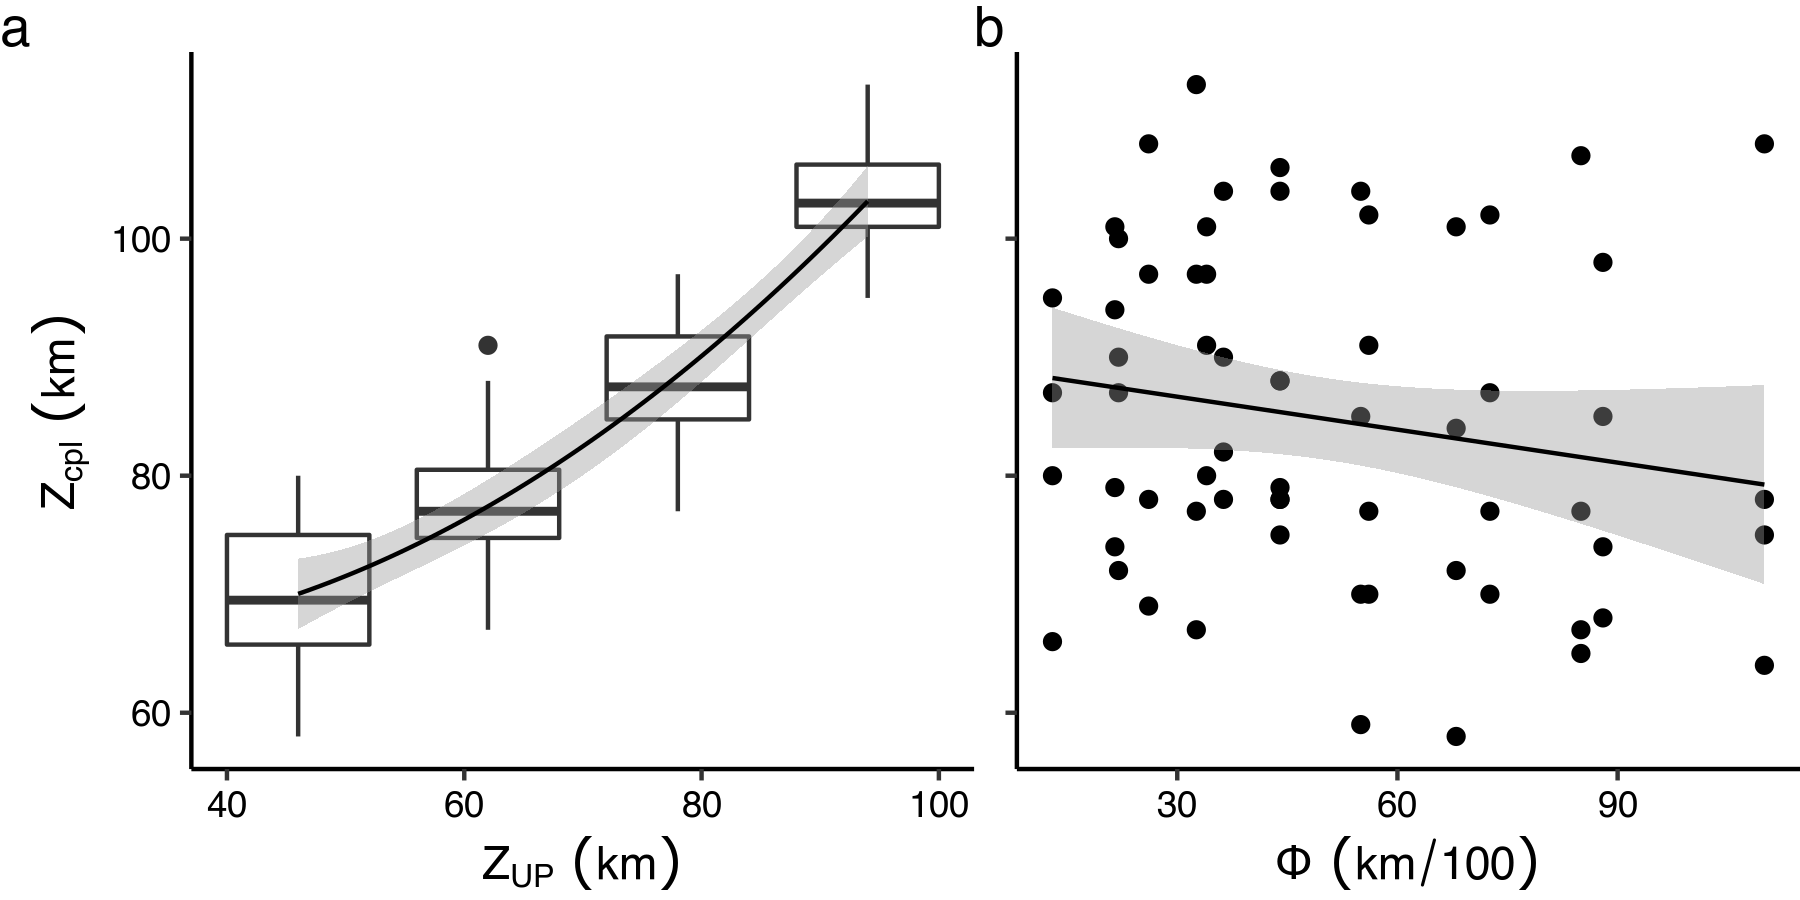
\includegraphics[width=1\linewidth,]{assets/figs/chpt2/fig5} 

}

\caption[Surface heat flow calculated from numerical experiments]{Surface heat flow ($\vec{q}$) vs. normalized distance for model cdf with upper-plate thickness ($Z_{UP}$) ranging from 46 to 94 $km$. The distribution of $\vec{q}$ in the forearc (normalized distance between 0.0 and 1.0) is narrow and shows little variance until near the arc (normalized distance between 0.75 and 1.0). The broad distribution of $\vec{q}$ behind the arc (normalized distance $>$ 1.0) reflects the broad distribution of initial continental geotherms ($Z_{UP}$). Any simple relationship between $\vec{q}$ and $Z_{UP}$ may be obscured by heating from extension or vertical migration of fluids, especially within the arc-region (high-amplitude fluctuations).}\label{fig:hf78}
\end{figure}

\gls{shf} across all numerical experiments is similar in the forearc region (normalized distance \(\leq\) 0.75, Figure \ref{fig:hf78}). In contrast, \gls{shf} extending behind the arc region (normalized distance \(>\) 0.75, Figure \ref{fig:hf78}) increases systematically, then levels off at values reflecting initial continental geotherms (i.e.~reflecting initial \gls{upt}). In reality, \gls{shf} depend on fault slip rates and rates of volcanic outputs. However, heat flow in the behind the arc may remain in steady-state if rates of volcanism and crustal thinning by extension are low (\protect\hyperlink{ref-currie2004}{Currie et al., 2004}; \protect\hyperlink{ref-currie2006}{Currie \& Hyndman, 2006}).

\hypertarget{chpt2Discussion}{%
\section{Discussion}\label{chpt2Discussion}}

\hypertarget{dynamic-feedbacks-regulating-plate-coupling}{%
\subsection{Dynamic feedbacks regulating plate coupling}\label{dynamic-feedbacks-regulating-plate-coupling}}

A clear association between plate coupling and the reaction \(antigorite \allowbreak \Leftrightarrow olivine + orthopyroxene + H_{2}O\) is observed in all experiments. A relatively narrow serpentine channel quickly forms above the dehydrating oceanic-plate, localizing strain, lubricating the plate interface, and inhibiting transfer of shear stress between plates (e.g., \protect\hyperlink{ref-agard2016}{Agard et al., 2016}; \protect\hyperlink{ref-ruh2015}{Ruh et al., 2015}). This mechanical behaviour is a direct consequence of a sharp rheologic change dependent on the location of serpentine dehydration reaction described in Section \ref{numHydration} and its effect on the rheologic model described in Section \ref{rheologicModel}. Interactions among viscosity changes, serpentine dehydration, and heat transfer are regulated by competing dynamic feedbacks acting in the upper plate. In summary, cooling and hydration of the shallow upper-plate mantle (serpentine stabilization) and heating from circulating asthenospheric mantle beneath the upper-plate lithosphere (driven by mechanical coupling) compete to stabilize \gls{cd} (Figure \ref{fig:flow}).

The entire process can be conceptualized with Figure \ref{fig:flow} as follows. The upper-plate mantle cools via diffusive heat loss to the oceanic-plate along the entire length of the plate interface (Figure @ref((fig:flow)a). At shallow depths, water released from the oceanic-plate stabilizes serpentine in the overriding upper-plate mantle, effectively decoupling the two plates (Figure \ref{fig:flow}b, point a). A positive feedback stabilizes serpentine to greater depths as decoupled plates stagnate the upper-plate mantle, promoting further cooling and formation of serpentine. Numerical experiments imply only a thin layer of serpentine is sufficient to trigger this feedback.

Deeper along the plate interface, beyond the stability of serpentine, diffusive heat loss from the upper-plate mantle to the slab forms a thickening layer of high-viscosity mantle atop the oceanic-plate (Figure \ref{fig:flow}b, point b). Downward motion of the oceanic-plate, plus accreted high-viscosity mantle (Figure \ref{fig:flow}b, point b) relative to the deepest extent of the stiff upper-plate mantle (Figure \ref{fig:flow}b, point c) creates a pressure gradient that attracts flow of the weakest materials---serpentine from the up-dip direction (Figure \ref{fig:flow}b, point d)---and hot mantle from below (Figure \ref{fig:flow}b, point e). Flow of hot mantle into the necking region between points b and c in Figure \ref{fig:flow} is analogous to passive asthenospheric upwelling toward a mid-ocean ridge where two strong cooling lithospheric plates diverge. Highly efficient heat advection from the warm upper-plate asthenospheric mantle (Figure \ref{fig:flow}a) prevents formation of sperentine---thus regulating and stabilizing the \gls{cd}.

Coupling mechanics apparent from numerical experiments can be described in terms of competing positive and negative feedbacks. The positive feedback involves addition of water into a diffusively cooling, shallow mantle to produce serpentine. The negative feedback involves serpentine destabilization by advection of heat from the deeper upper-plate asthenospheric mantle. Such thermal-petrologic-mechanical feedbacks drive \gls{cd} towards steady-state. Our results imply a finely-tuned balance of serpentine stability can maintain \glspl{cd} in glspl\{sz\} for potentially 10's of Ma.

\hypertarget{cplResponses}{%
\subsection{\texorpdfstring{Coupling responses to \(Z_{UP}\) and \(\Phi\)}{Coupling responses to Z\_\{UP\} and \textbackslash Phi}}\label{cplResponses}}

How does \gls{upt} influence \gls{cd}? Numerical experiments point to the upper-plate lithosphere-asthenosphere boundary as an important feature constraining coupling mechanics as it defines the permissible flow field in the upper-plate (Figure \ref{fig:streams}a-d). Thin upper-plate lithospheres (Figure \ref{fig:streams}a, b) permit shallow mantle flow and advection of heat farther up the plate interface. Thin upper-plate lithospheres thereby raise coupling depths by raising serpentine stability up the plate interface. Thick upper-plate lithospheres (Figure \ref{fig:streams}c, d) restrict mantle wedge flow to deeper levels, deepening serpentine stability and mechanical coupling.

The thermal state of the slab, as represented by \(\Phi\), has almost no effect on \gls{cd} by comparison. Relative insensitivity of \gls{cd} to \(\Phi\) is consistent with previous studies of active \glspl{sz} (\protect\hyperlink{ref-furukawa1993}{Furukawa, 1993}; \protect\hyperlink{ref-wada2009}{Wada \& Wang, 2009}). The irresponsiveness of \gls{cd} to changes in \(\Phi\) is perhaps due to competing cooling and heating effects driven by the subducting oceanic-plate. For example, high-\(\Phi\) oceanic-plates (older plates with higher velocities) cool the upper-plate mantle more effectively, but also effectively heat the interface by driving stronger mantle circulation. In contrast, low-\(\Phi\) oceanic-plates (younger plates with lower velocities) are less effective in cooling the upper-plate mantle, but also ineffectively heat the interface by ineffectively driving mantle circulation. That is, the shallow vs.~deep dynamic effects of \(\Phi\) tend to cancel each other, explaining the lack of correlation between \gls{cd} and \(\Phi\).

\begin{figure}[htbp]

{\centering 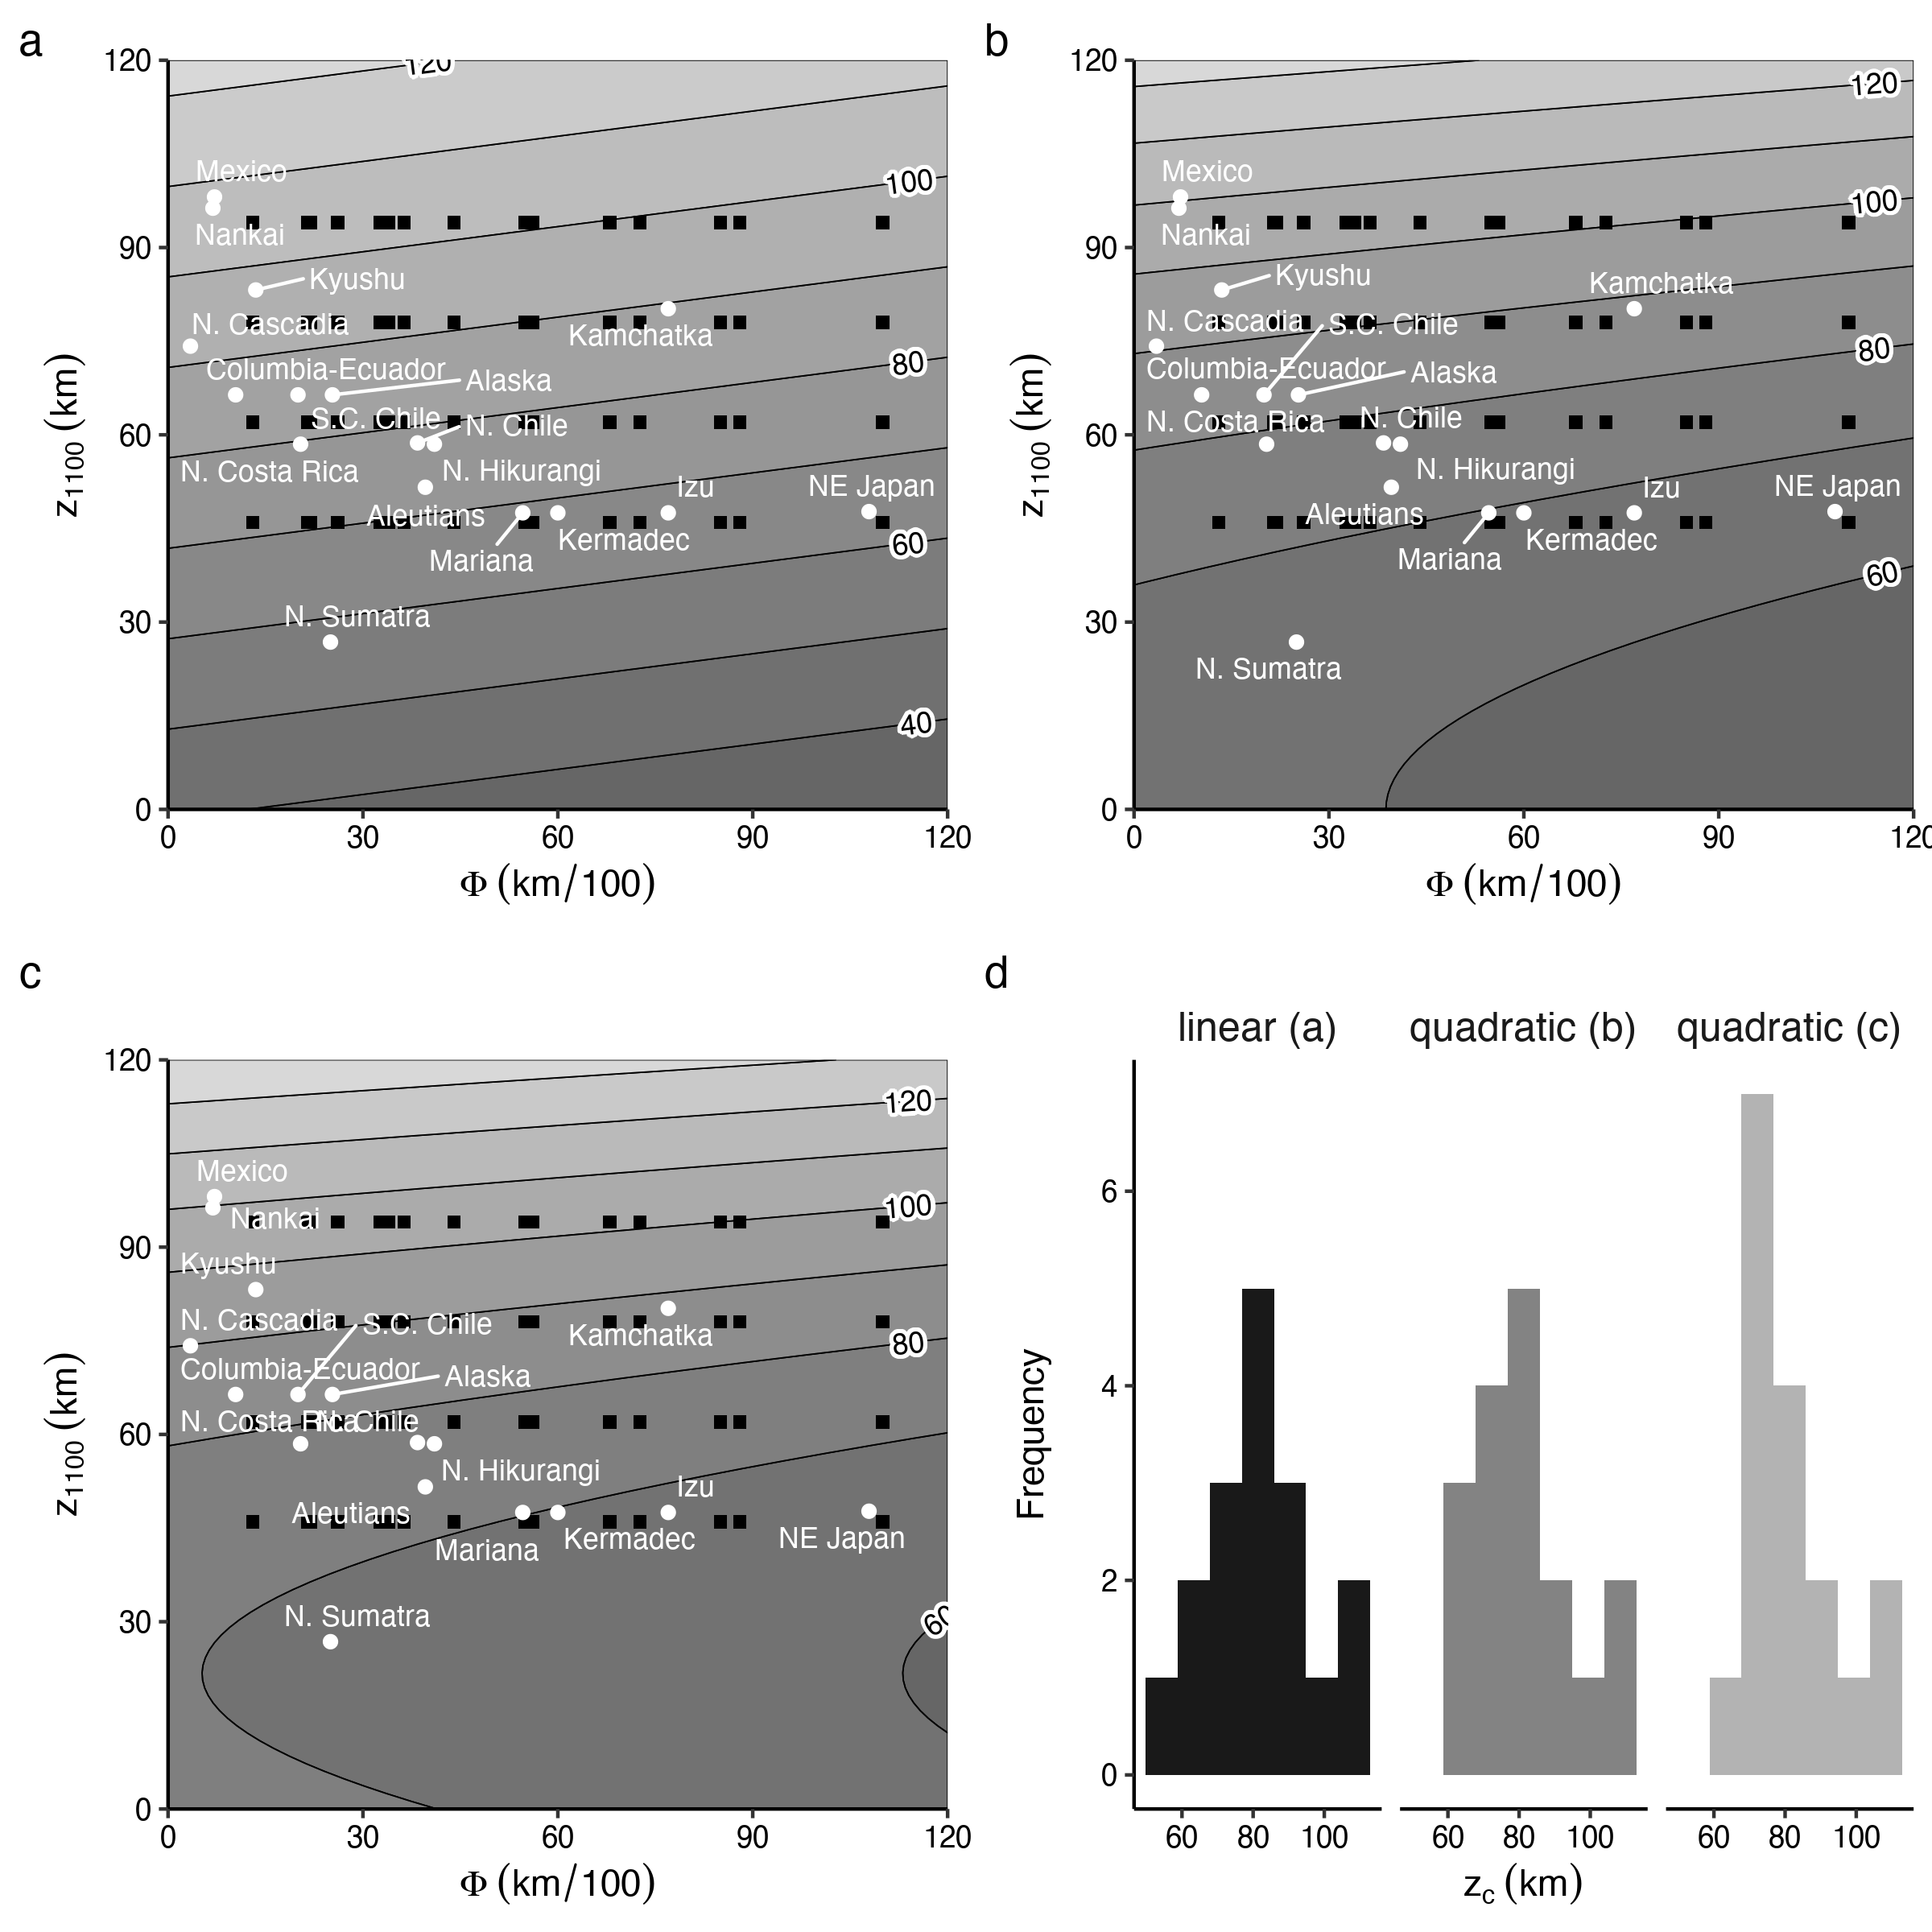
\includegraphics[width=1\linewidth,]{assets/figs/chpt2/fig6} 

}

\caption[Visualizing viscosity and mantle flow]{Visualizing viscosity and mantle flow near the coupling region at approximately 10 $Ma$ for model cdf with upper-plate thickness of 78 $km$. Strong mantle flow beneath the lithospheric base (1100$^{\circ}C$) transfers heat towards the coupling region. Viscosity indicates coupling at the point where the viscosity contrast between the slab and mantle approaches zero (between points b \& d). Reference points a-e are used for discussing coupling dynamics and thermal feedbacks (see Section \ref{cplResponses}).}\label{fig:flow}
\end{figure}

\hypertarget{estimating-coupling-depths-in-subduction-zones}{%
\subsection{Estimating coupling depths in subduction zones}\label{estimating-coupling-depths-in-subduction-zones}}

Theoretically, \gls{cd} can be estimated directly by fitting forearc \gls{shf} data using forward modelling approaches (e.g., \protect\hyperlink{ref-wada2009}{Wada \& Wang, 2009}). However, forward approaches typically adjust \gls{cd} independently from \gls{upt}, which is inconsistent with an inherent link between \gls{cd} and \gls{upt} discussed in Section \ref{chpt2Discussion} (e.g., Figures \ref{fig:hf78} \& \ref{fig:streams}). Moreover, many additional heat sources (e.g., shear heating and crustal plutonism, \protect\hyperlink{ref-gao2014}{Gao \& Wang, 2014}; \protect\hyperlink{ref-reesjones2018}{Rees Jones et al., 2018}) may contribute to forearc \gls{shf}---increasing uncertainty when inverting \gls{upt} from \gls{shf}.

Assuming low degrees of backarc extension, estimating \gls{cd} in active \glspl{sz} using Equation \eqref{eq:zCpl} with \(Z_{UP}\) inverted from backarc \gls{shf} is preferable to avoid additional uncertainties stemming from seismic and volcanic activity in the forearc. However, while \(\Phi\) is inventoried for most active \glspl{sz} (\protect\hyperlink{ref-syracuse2006}{Syracuse \& Abers, 2006}), a corresponding dataset of \(Z_{UP}\) does not exist. Several geophysical and petrologic methods might be considered for independent estimates of \(Z_{UP}\) (e.g., seismic velocities, flexure, heat flow, mantle xenoliths). Backarc \gls{shf} is still a good choice, however, because of its direct correspondence with \(Z_{UP}\). For example, \(Z_{UP}\) may be estimated using simple one-dimensional heat transport models assuming values for radiogenic heat production in the crust (\protect\hyperlink{ref-rudnick1998}{Rudnick et al., 1998}). Special attention must be paid to crustal processes, including extension and magmatism, because additional heating will underestimate \(Z_{UP}\) and, consequently, underestimate \gls{cd}.

\begin{figure}[htbp]

{\centering 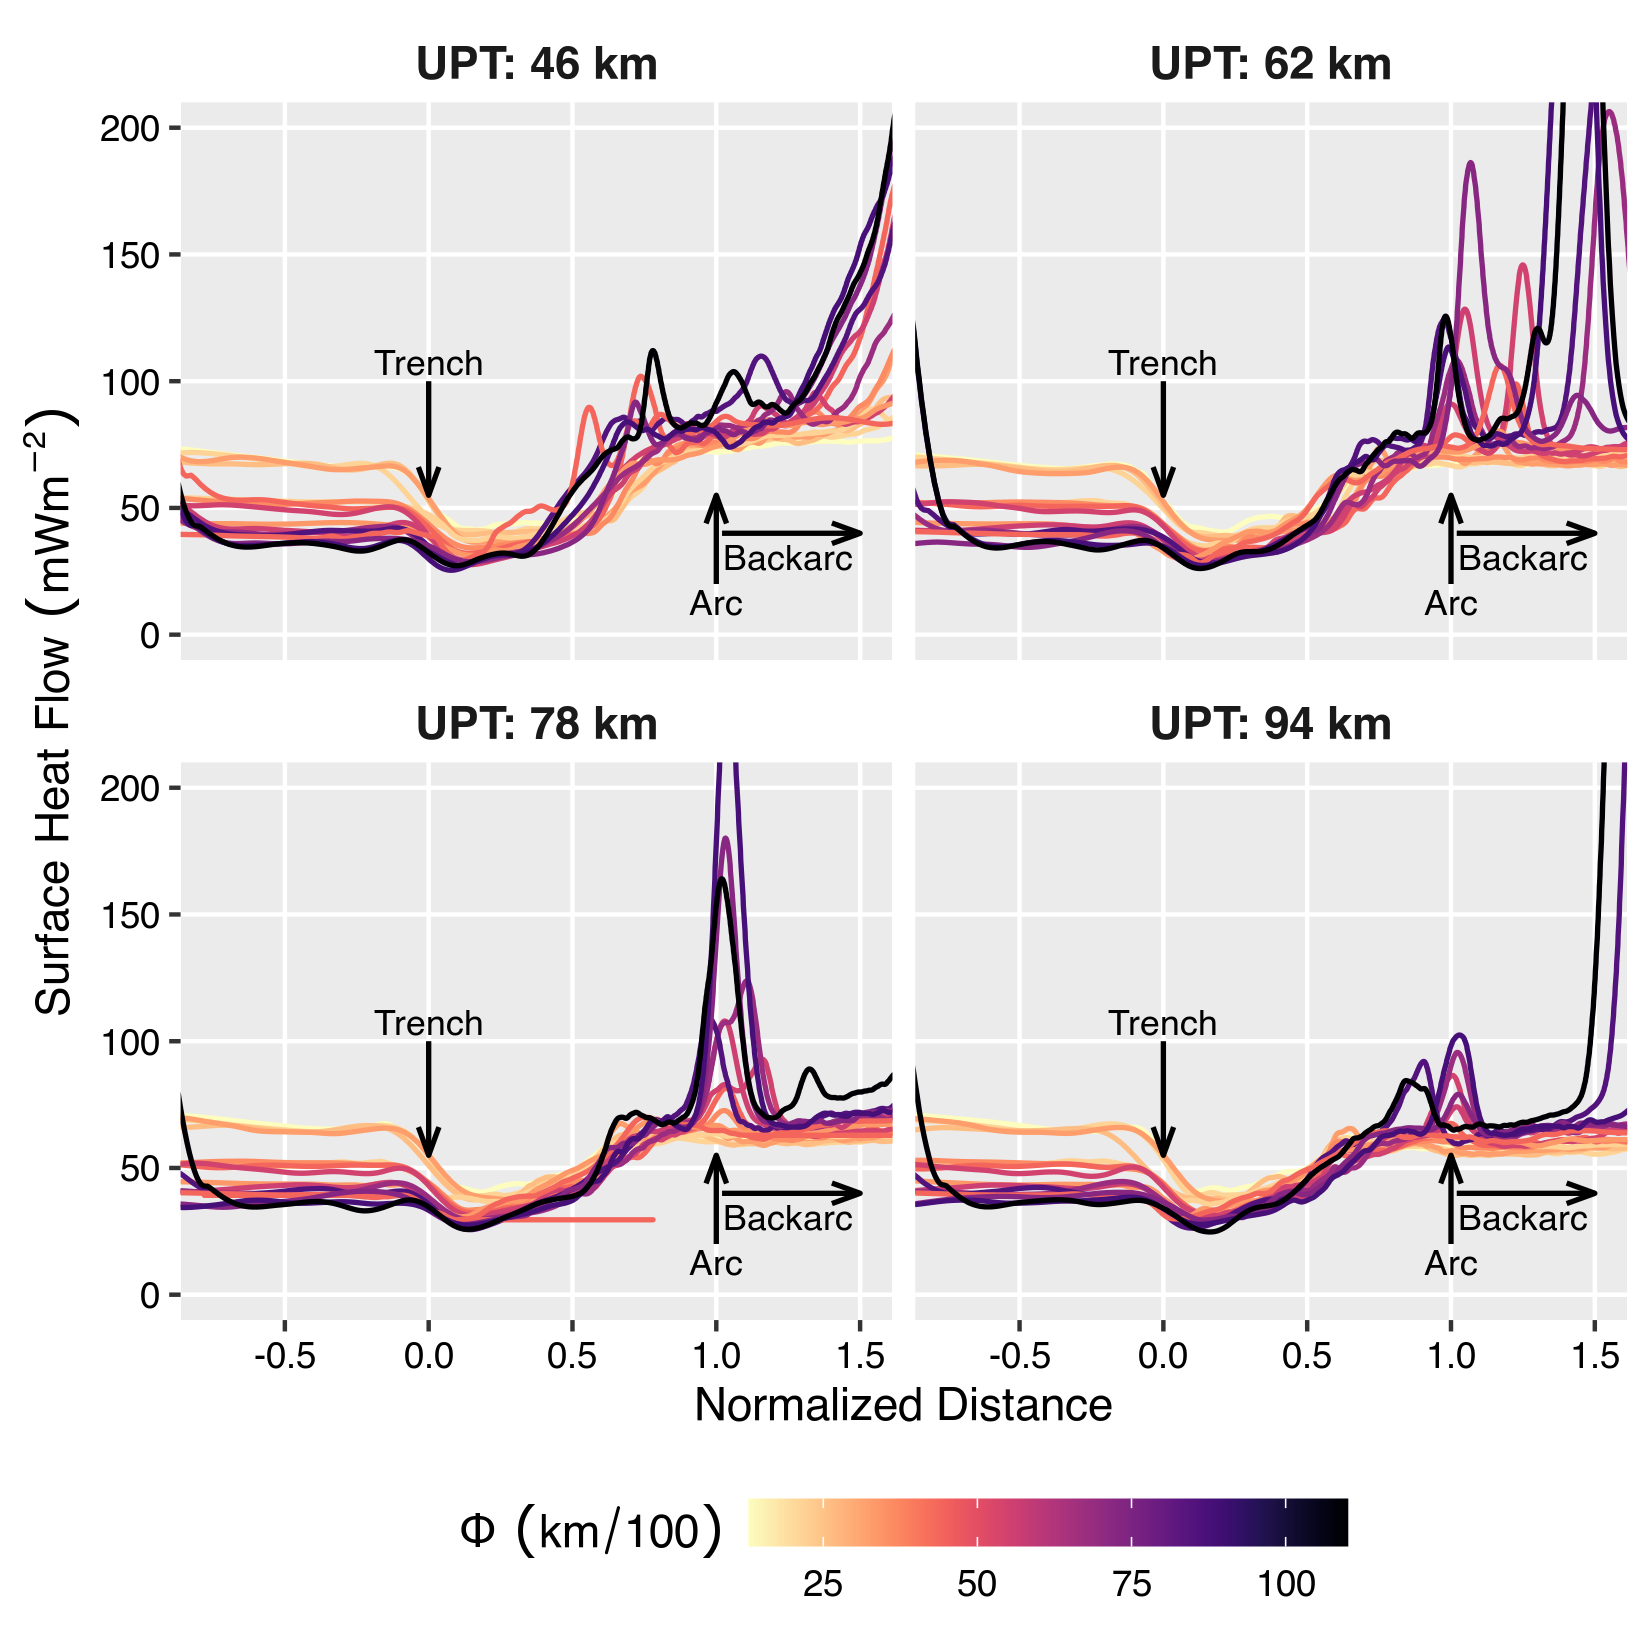
\includegraphics[width=1\linewidth,]{assets/figs/chpt2/fig7} 

}

\caption[Visualizing mantle flow and coupling by upper-plate thickness]{Visualizing mantle flow at approximately 10 $Ma$ for model cdf with upper-plate thickness of (a) 46, (b) 62, (c) 78, and (d) 94 $km$. All experiments are plotted on the same scale and location within the model domain. The flow of warm mantle is restricted to below the 1100$^{\circ}C$ isotherm, which corresponds to the base of the upper-plate lithosphere ($Z_{UP}$). A minimum coupling depth ($Z_{cpl}$) appears to exist as models with extremely thin lithospheres (a) exhibit coupling at $\sim$ 70-80 $km$ depth. $Z_{cpl}$ generally increases with increasing $Z_{UP}$ as mantle flow and advective heat transport are restricted to greater depths.}\label{fig:streams}
\end{figure}

\hypertarget{globally-similar-coupling-depths}{%
\subsection{Globally similar coupling depths?}\label{globally-similar-coupling-depths}}

A \(Z_{cpl}\) distribution of 82 \(\pm\) 14 \(km\) (2\(\sigma\)) estimated for active \glspl{sz} in this study (Figure \ref{fig:multiv}d) roughly match the preferred \(Z_{cpl}\) inferred from forearc \gls{shf} for Cascadia and NE Japan (75-80 \(km\), \protect\hyperlink{ref-syracuse2010}{Syracuse et al., 2010}; \protect\hyperlink{ref-wada2009}{Wada \& Wang, 2009}) \(km\). The range of \(Z_{cpl}\) estimated for active \glspl{sz} in this study (Figure \ref{fig:multiv}d) is relatively broad, however. For example, omitting Mexico and Nankai because their \(\Phi\) values fall outside our modeling domain, estimated \glspl{cd} range from almost 100 \(km\) (Kyushu) to approximately 65 \(km\) (Sumatra and NE Japan, Table \ref{tab:segs}).

\gls{cd} in active \glspl{sz} are commonly assumed to be narrowly distributed around 70-80 \(km\) (\protect\hyperlink{ref-syracuse2010}{Syracuse et al., 2010}; \protect\hyperlink{ref-wada2009}{Wada \& Wang, 2009}). The strong correlation between \(Z_{UP}\) and \(Z_{cpl}\) found from numerical experiments imply uniform \glspl{cd} are possible if \gls{upt} are globally uniform. The \gls{shf} dataset compiled by Wada \& Wang (\protect\hyperlink{ref-wada2009}{2009}) (Table \ref{tab:segs}) shows average backarc \gls{shf} are indeed similar among active \glspl{sz}---implying a narrow distribution of \glspl{cd} (Figure \ref{fig:multiv}d). Much of their dataset is based on Currie \& Hyndman (\protect\hyperlink{ref-currie2006}{2006}), who estimate \gls{upt} for 10 circum-Pacific subduction zones of 50-60 \(km\) (defined by the 1200 \(^{\circ}C\) isotherm). Uniformly thin \gls{upt} are corroborated by uniformly high heat flow (\(>\) 70 \(mW/m^{2}\)), thermobarometric constraints on mantle xenoliths, and P-wave velocities (\protect\hyperlink{ref-currie2006}{Currie \& Hyndman, 2006}). An attempt is made to further corroborate the uniformity of \gls{upt} in Chapter \ref{chpt3} by interpolating \gls{shf} near active \glspl{sz}.

Although it still curious why upper-plates among \glspl{sz} may have similar thicknesses, one can assume it is likely related to some processes of lithospheric erosion proposed for subarc lithosphere. These include: lithospheric delamination induced by lower crust eclogitization (\protect\hyperlink{ref-sobolev2005}{Sobolev \& Babeyko, 2005}), small-scale convection caused by hydration-induced mantle wedge weakening (\protect\hyperlink{ref-arcay2006}{Arcay et al., 2006}), thermal erosion (\protect\hyperlink{ref-england2010}{England \& Katz, 2010}), mechanical weakening by percolating melts (\protect\hyperlink{ref-gerya2011}{Gerya \& Meilick, 2011}), and subarc foundering of magmatic cumulates (\protect\hyperlink{ref-jull2001}{Jull \& Kelemen, 2001}). Most of these mechanisms are thus strongly related to mantle wedge hydration, melting, and melt transport toward volcanic arcs.

The metamorphic rock record may also imply consistency among \glspl{cd} in \glspl{sz}. For example, the demise of a serpentine channel and onset of coupling may provide a natural barrier such that rocks are more likely to be exhumed from within the channel than from below it. The relative abundance of blueschists and eclogites should then be greater for pressures below estimated \glspl{cd} (approximately 2.4 \(GPa\) or 70-80 \(km\)) than above them. This hypothesis will be explicitly explored in Chapter \ref{chpt4}.

\hypertarget{conclusions}{%
\section{Conclusions}\label{conclusions}}

Three important results are highlighted in this study:

\begin{enumerate}
\def\labelenumi{\arabic{enumi}.}
\item
  \gls{cd} is stabilized near the base of the upper-plate lithosphere by competing dynamic feedbacks regulating heat transport, serpentine dehydration, and mechanical coupling in the upper-plate mantle.
\item
  A simple expression fitted to \glspl{cd} observed in numerical experiments allows the \glspl{cd} to be estimated for active \glspl{sz} by inverting \gls{upt} from \gls{shf}.
\item
  Uniform \gls{shf} in circum-Pacific subduction zones (\protect\hyperlink{ref-currie2006}{Currie \& Hyndman, 2006}; \protect\hyperlink{ref-wada2009}{Wada \& Wang, 2009}) may indicate uniform \glspl{cd} at approximately 80 \(km\).
\end{enumerate}

Questions remain, however, including: how do warm (thin) upper-plates persist over 100's of kilometers behind arcs and throughout the lifespan of subduction zones? How abruptly are dehydration reaction occurring along the subduction interface? How can expressions like Equation \eqref{eq:zCpl} be improved using natural datasets? Each of these questions may be good candidates for future research.

\cleardoublepage

\hypertarget{chpt3}{%
\chapter{A Comparison of Heat Flow Interpolations Near Subduction Zones}\label{chpt3}}

\markboth{Chapter 3: Heat Flow Interpolations}{Chapter 3: Heat Flow Interpolations}

\begin{quote}
\textbf{Keypoints:}

\begin{itemize}
\item
  Inconsistent spatial patterns characterize heat flow near \glspl{sz}
\item
  Heat flow investigations favour 2D interpolations over 1D transects
\item
  Scaling datasets and new interpolation schema will advance \gls{sz} research
\end{itemize}
\end{quote}

\hypertarget{abstract-1}{%
\section{Abstract}\label{abstract-1}}

Heat fluxing through the Earth's surface provides indirect observations of \glsfirst{pts} fields deep in \glspl{sz}. Global heat flow databases, therefore, are invaluable for generating and testing belief about \gls{sz} geodynamics. Investigating \glsfirst{shf} in two-dimensions by interpolation, rather than in one-dimension by projection, arguably forms better interpretations about spatial continuity of deep processes. Direct comparisons of interpolations based on the First (spatial continuity) and Third (similarity) Laws of Geography applied to the most updated global heat flow database. Inconsistent spatial patterns of \gls{shf} near \glspl{sz} are observed in magnitude and variance, regardless of interpolation method. The implications include discontinuous \gls{pts} fields at depth, countering hypotheses of commonly thin upper plate lithospheres and mechanical \glspl{cd} among \glspl{sz}. Strategic scaling of \gls{shf} datasets will improve interpolation precision and confidence---leading to better tools for distinguishing differences within and among \glspl{sz}. New data acquisition and composite interpolation schema are proposed as avenues for future \gls{sz} research.

\hypertarget{introduction-2}{%
\section{Introduction}\label{introduction-2}}

Heat escaping the solid Earth's surface indicates a dynamically cooling planet. Surface heat flow databases (\protect\hyperlink{ref-hasterok2008}{Hasterok \& Chapman, 2008}; \protect\hyperlink{ref-lucazeau2019}{Lucazeau, 2019}; \protect\hyperlink{ref-pollack1993}{Pollack et al., 1993}) enable investigations and quantification geodynamics by relating the amount of heat escaping Earth's surface to heat-transferring and heat-generating subsurface processes such as diffusion, hydrothermal circulation, radioactive decay, fault motion, subduction dynamics, and mantle convection (\protect\hyperlink{ref-currie2004}{Currie et al., 2004}; \protect\hyperlink{ref-currie2006}{Currie \& Hyndman, 2006}; \protect\hyperlink{ref-fourier1827}{Fourier, 1827}; \protect\hyperlink{ref-furlong2013}{Furlong \& Chapman, 2013}; \protect\hyperlink{ref-furukawa1993}{Furukawa, 1993}; \protect\hyperlink{ref-gao2014}{Gao \& Wang, 2014}; \protect\hyperlink{ref-hasterok2013}{Hasterok, 2013}; \protect\hyperlink{ref-kerswell2020}{Kerswell et al., 2020}; \protect\hyperlink{ref-parsons1977}{Parsons \& Sclater, 1977}; \protect\hyperlink{ref-pollack1977}{Pollack \& Chapman, 1977}; \protect\hyperlink{ref-rudnick1998}{Rudnick et al., 1998}; \protect\hyperlink{ref-stein1992}{Stein \& Stein, 1992}, \protect\hyperlink{ref-stein1994}{1994}; \protect\hyperlink{ref-wada2009}{Wada \& Wang, 2009}). Surface heat flow observations continue to motivate research, evident by more than 1,393 publications compiled in the most recent heat flow database, although the rate of publications using surface heat flow has declined since the mid 1980's (\protect\hyperlink{ref-jennings2021}{Jennings \& Hasterok, 2021}).

\cleardoublepage

\hypertarget{references}{%
\chapter*{References}\label{references}}
\addcontentsline{toc}{chapter}{References}

\markboth{References}{References}

\hypertarget{refs}{}
\begin{CSLReferences}{1}{1}
\leavevmode\vadjust pre{\hypertarget{ref-abers2017}{}}%
Abers, G., van Keken, P., \& Hacker, B. (2017). The cold and relatively dry nature of mantle forearcs in subduction zones. \emph{Nature Geoscience}, \emph{10}(5), 333--337.

\leavevmode\vadjust pre{\hypertarget{ref-agard2009}{}}%
Agard, P., Yamato, P., Jolivet, L., \& Burov, E. (2009). Exhumation of oceanic blueschists and eclogites in subduction zones: Timing and mechanisms. \emph{Earth-Science Reviews}, \emph{92}(1-2), 53--79.

\leavevmode\vadjust pre{\hypertarget{ref-agard2016}{}}%
Agard, P., Yamato, P., Soret, M., Prigent, C., Guillot, S., Plunder, A., et al. (2016). Plate interface rheological switches during subduction infancy: Control on slab penetration and metamorphic sole formation. \emph{Earth and Planetary Science Letters}, \emph{451}, 208--220.

\leavevmode\vadjust pre{\hypertarget{ref-agard2018}{}}%
Agard, P., Plunder, A., Angiboust, S., Bonnet, G., \& Ruh, J. (2018). The subduction plate interface: Rock record and mechanical coupling (from long to short time scales). \emph{Lithos}, \emph{320-321}, 537--566.

\leavevmode\vadjust pre{\hypertarget{ref-agrusta2013}{}}%
Agrusta, R., Arcay, D., Tommasi, A., Davaille, A., Ribe, N., \& Gerya, T. (2013). Small-scale convection in a plume-fed low-viscosity layer beneath a moving plate. \emph{Geophysical Journal International}, \emph{194}(2), 591--610.

\leavevmode\vadjust pre{\hypertarget{ref-angiboust2012a}{}}%
Angiboust, S., Langdon, R., Agard, P., Waters, D., \& Chopin, C. (2012). Eclogitization of the monviso ophiolite (w. Alps) and implications on subduction dynamics. \emph{Journal of Metamorphic Geology}, \emph{30}(1), 37--61.

\leavevmode\vadjust pre{\hypertarget{ref-angiboust2014}{}}%
Angiboust, S., Pettke, T., De Hoog, J., Caron, B., \& Oncken, O. (2014). Channelized fluid flow and eclogite-facies metasomatism along the subduction shear zone. \emph{Journal of Petrology}, \emph{55}(5), 883--916.

\leavevmode\vadjust pre{\hypertarget{ref-arcay2006}{}}%
Arcay, D., Doin, M., Tric, E., Bousquet, R., \& de Capitani, C. (2006). Overriding plate thinning in subduction zones: Localized convection induced by slab dehydration. \emph{Geochemistry, Geophysics, Geosystems}, \emph{7}(2).

\leavevmode\vadjust pre{\hypertarget{ref-burg2005}{}}%
Burg, J., \& Gerya, T. (2005). The role of viscous heating in barrovian metamorphism of collisional orogens: Thermomechanical models and application to the lepontine dome in the central alps. \emph{Journal of Metamorphic Geology}, \emph{23}(2), 75--95.

\leavevmode\vadjust pre{\hypertarget{ref-carlson2003}{}}%
Carlson, R., \& Miller, D. (2003). Mantle wedge water contents estimated from seismic velocities in partially serpentinized peridotites. \emph{Geophysical Research Letters}, \emph{30}(5).

\leavevmode\vadjust pre{\hypertarget{ref-cizkova2013}{}}%
Čížková, H., \& Bina, C. (2013). Effects of mantle and subduction-interface rheologies on slab stagnation and trench rollback. \emph{Earth and Planetary Science Letters}, \emph{379}, 95--103.

\leavevmode\vadjust pre{\hypertarget{ref-connolly2005}{}}%
Connolly, J. (2005). Computation of phase equilibria by linear programming: A tool for geodynamic modeling and its application to subduction zone decarbonation. \emph{Earth and Planetary Science Letters}, \emph{236}(1-2), 524--541.

\leavevmode\vadjust pre{\hypertarget{ref-currie2006}{}}%
Currie, C., \& Hyndman, R. (2006). The thermal structure of subduction zone back arcs. \emph{Journal of Geophysical Research: Solid Earth}, \emph{111}(B8), 1--22.

\leavevmode\vadjust pre{\hypertarget{ref-currie2004}{}}%
Currie, C., Wang, K., Hyndman, R., \& He, J. (2004). The thermal effects of steady-state slab-driven mantle flow above a subducting plate: The cascadia subduction zone and backarc. \emph{Earth and Planetary Science Letters}, \emph{223}(1-2), 35--48.

\leavevmode\vadjust pre{\hypertarget{ref-davies1999}{}}%
Davies, J. (1999). The role of hydraulic fractures and intermediate depth earthquakes in generating suduction zone magmatism. \emph{Nature}, \emph{417}(March), 142--145.

\leavevmode\vadjust pre{\hypertarget{ref-england2010}{}}%
England, P., \& Katz, R. (2010). Melting above the anhydrous solidus controls the location of volcanic arcs. \emph{Nature}, \emph{467}(7316), 700--703.

\leavevmode\vadjust pre{\hypertarget{ref-england2004}{}}%
England, P., Engdahl, R., \& Thatcher, W. (2004). Systematic variation in the depths of slabs beneath arc volcanoes. \emph{Geophysical Journal International}, \emph{156}(2), 377--408.

\leavevmode\vadjust pre{\hypertarget{ref-faccenda2009}{}}%
Faccenda, M., Gerya, T., \& Burlini, L. (2009). Deep slab hydration induced by bending-related variations in tectonic pressure. \emph{Nature Geoscience}, \emph{2}(11), 790--793.

\leavevmode\vadjust pre{\hypertarget{ref-fourier1827}{}}%
Fourier, J. (1827). M{é}moire sur les temp{é}ratures du globe terrestre et des espaces plan{é}taires. \emph{M{é}moires de l'Acad{é}mie Royale Des Sciences de l'Institut de France}, \emph{7}, 570--604.

\leavevmode\vadjust pre{\hypertarget{ref-furlong2013}{}}%
Furlong, K., \& Chapman, D. (2013). Heat flow, heat generation, and the thermal state of the lithosphere. \emph{Annual Review of Earth and Planetary Sciences}, \emph{41}(1), 385--410.

\leavevmode\vadjust pre{\hypertarget{ref-furukawa1993}{}}%
Furukawa, Y. (1993). Depth of the decoupling plate interface and thermal structure under arcs. \emph{Journal of Geophysical Research: Solid Earth}, \emph{98}(B11), 20005--20013.

\leavevmode\vadjust pre{\hypertarget{ref-gao2014}{}}%
Gao, X., \& Wang, K. (2014). Strength of stick-slip and creeping subduction megathrusts from heat flow observations. \emph{Science}, \emph{345}(6200), 1038--1041.

\leavevmode\vadjust pre{\hypertarget{ref-gao2017}{}}%
Gao, X., \& Wang, K. (2017). Rheological separation of the megathrust seismogenic zone and episodic tremor and slip. \emph{Nature}, \emph{543}(7645), 416--419.

\leavevmode\vadjust pre{\hypertarget{ref-gerya2011}{}}%
Gerya, T., \& Meilick, F. (2011). Geodynamic regimes of subduction under an active margin: Effects of rheological weakening by fluids and melts. \emph{Journal of Metamorphic Geology}, \emph{29}(1), 7--31.

\leavevmode\vadjust pre{\hypertarget{ref-gerya2003}{}}%
Gerya, T., \& Yuen, D. (2003). Characteristics-based marker-in-cell method with conservative finite-differences schemes for modeling geological flows with strongly variable transport properties. \emph{Physics of the Earth and Planetary Interiors}, \emph{140}(4), 293--318.

\leavevmode\vadjust pre{\hypertarget{ref-gerya2008}{}}%
Gerya, T., Connolly, J., \& Yuen, D. (2008). Why is terrestrial subduction one-sided? \emph{Geology}, \emph{36}(1), 43--46.

\leavevmode\vadjust pre{\hypertarget{ref-gonzalez2016}{}}%
Gonzalez, C., Gorczyk, W., \& Gerya, T. (2016). Decarbonation of subducting slabs: Insight from petrological--thermomechanical modeling. \emph{Gondwana Research}, \emph{36}, 314--332.

\leavevmode\vadjust pre{\hypertarget{ref-gorczyk2007}{}}%
Gorczyk, W., Willner, A., Gerya, T., Connolly, J., \& Burg, J. (2007). Physical controls of magmatic productivity at pacific-type convergent margins: Numerical modelling. \emph{Physics of the Earth and Planetary Interiors}, \emph{163}(1-4), 209--232.

\leavevmode\vadjust pre{\hypertarget{ref-grove2012}{}}%
Grove, T., Till, C., \& Krawczynski, M. (2012). The role of \(H_2O\) in subduction zone magmatism. \emph{Annual Review of Earth and Planetary Sciences}, \emph{40}(1), 413--439.

\leavevmode\vadjust pre{\hypertarget{ref-hacker2003}{}}%
Hacker, B., Abers, G., \& Peacock, S. (2003). Subduction factory 1. Theoretical mineralogy, densities, seismic wave speeds, and \(H_2O\) contents. \emph{Journal of Geophysical Research: Solid Earth}, \emph{108}(B1).

\leavevmode\vadjust pre{\hypertarget{ref-harlow1962}{}}%
Harlow, F. (1962). \emph{The particle-in-cell method for numerical solution of problems in fluid dynamics}. Los Alamos Scientific Lab., N. Mex.

\leavevmode\vadjust pre{\hypertarget{ref-harlow1964}{}}%
Harlow, F. (1964). The particle-in-cell computing method for fluid dynamics. \emph{Methods Comput. Phys.}, \emph{3}, 319--343.

\leavevmode\vadjust pre{\hypertarget{ref-hasterok2013}{}}%
Hasterok, D. (2013). A heat flow based cooling model for tectonic plates. \emph{Earth and Planetary Science Letters}, \emph{361}, 34--43.

\leavevmode\vadjust pre{\hypertarget{ref-hasterok2008}{}}%
Hasterok, D., \& Chapman, D. (2008). Global heat flow: A new database and a new approach. In \emph{AGU fall meeting abstracts} (Vol. 2008, pp. T21c--1985).

\leavevmode\vadjust pre{\hypertarget{ref-hilairet2007}{}}%
Hilairet, N., Reynard, B., Wang, Y., Daniel, I., Merkel, S., Nishiyama, N., \& Petitgirard, S. (2007). High-pressure creep of serpentine, interseismic deformation, and initiation of subduction. \emph{Science}, \emph{318}(5858), 1910--1913.

\leavevmode\vadjust pre{\hypertarget{ref-hirauchi2010}{}}%
Hirauchi, K., Katayama, I., Uehara, S., Miyahara, M., \& Takai, Y. (2010). Inhibition of subduction thrust earthquakes by low-temperature plastic flow in serpentine. \emph{Earth and Planetary Science Letters}, \emph{295}(3-4), 349--357.

\leavevmode\vadjust pre{\hypertarget{ref-hyndman2003}{}}%
Hyndman, R., \& Peacock, S. (2003). Serpentinization of the forearc mantle. \emph{Earth and Planetary Science Letters}, \emph{212}(3-4), 417--432.

\leavevmode\vadjust pre{\hypertarget{ref-ito1971}{}}%
Ito, K., \& Kennedy, G. (1971). An experimental study of the basalt-garnet granulite-eclogite transition. \emph{The Structure and Physical Properties of the Earth's Crust}, \emph{14}, 303--314.

\leavevmode\vadjust pre{\hypertarget{ref-jennings2021}{}}%
Jennings, S., \& Hasterok, D. (2021). HeatFlow.org. \emph{Heatflow.org}. Retrieved from \url{http://heatflow.org/}

\leavevmode\vadjust pre{\hypertarget{ref-jull2001}{}}%
Jull, M., \& Kelemen, P. (2001). On the conditions for lower crustal convective instability. \emph{Journal of Geophysical Research: Solid Earth}, \emph{106}(b4), 6423--6446.

\leavevmode\vadjust pre{\hypertarget{ref-karato1993}{}}%
Karato, S., \& Wu, P. (1993). Rheology of the upper mantle: A synthesis. \emph{Science}, \emph{260}(5109), 771--778.

\leavevmode\vadjust pre{\hypertarget{ref-kerswell2020}{}}%
Kerswell, B., Kohn, M., \& Gerya, T. (2020). Backarc lithospheric thickness and serpentine stability control slab-mantle coupling depths in subduction zones. \emph{Geochemistry, Geophysics, Geosystems}, e2020GC009304.

\leavevmode\vadjust pre{\hypertarget{ref-lucazeau2019}{}}%
Lucazeau, F. (2019). Analysis and mapping of an updated terrestrial heat flow data set. \emph{Geochemistry, Geophysics, Geosystems}, \emph{20}(8), 4001--4024.

\leavevmode\vadjust pre{\hypertarget{ref-mckenzie1969}{}}%
McKenzie, D. (1969). Speculations on the consequences and causes of plate motions. \emph{Geophysical Journal International}, \emph{18}(1), 1--32.

\leavevmode\vadjust pre{\hypertarget{ref-parsons1977}{}}%
Parsons, B., \& Sclater, J. (1977). An analysis of the variation of ocean floor bathymetry and heat flow with age. \emph{Journal of Geophysical Research}, \emph{82}(5), 803--827.

\leavevmode\vadjust pre{\hypertarget{ref-peacock1990}{}}%
Peacock, S. (1990). Fluid processes in subduction zones. \emph{Science}, \emph{248}(4953), 329--337.

\leavevmode\vadjust pre{\hypertarget{ref-peacock1991}{}}%
Peacock, S. (1991). Numerical simulation of subduction zone pressure-temperature-time paths: Constraints on fluid production and arc magmatism. \emph{Philosophical Transactions of the Royal Society of London. Series A: Physical and Engineering Sciences}, \emph{335}(1638), 341--353.

\leavevmode\vadjust pre{\hypertarget{ref-peacock1993}{}}%
Peacock, S. (1993). The importance of blueschist \(\rightarrow\) eclogite dehydration reactions in subducting oceanic crust. \emph{Geological Society of America Bulletin}, \emph{105}(5), 684--694.

\leavevmode\vadjust pre{\hypertarget{ref-peacock1996}{}}%
Peacock, S. (1996). Thermal and petrologic structure of subduction zones. \emph{Subduction: Top to Bottom}, \emph{96}, 119--133.

\leavevmode\vadjust pre{\hypertarget{ref-peacock1999a}{}}%
Peacock, S., \& Hyndman, R. (1999). Hydrous minerals in the mantle wedge and the maximum depth of subduction thrust earthquakes. \emph{Geophysical Research Letters}, \emph{26}(No. 16), 2517--2520.

\leavevmode\vadjust pre{\hypertarget{ref-peacock1999b}{}}%
Peacock, S., \& Wang, K. (1999). Seismic consequences of warm versus cool subduction metamorphism: Examples from southwest and northeast japan. \emph{Science}, \emph{286}(5441), 937--939.

\leavevmode\vadjust pre{\hypertarget{ref-peacock1994}{}}%
Peacock, S., Rushmer, T., \& Thompson, A. (1994). Partial melting of subducting oceanic crust. \emph{Earth and Planetary Science Letters}, \emph{121}(1-2), 227--244.

\leavevmode\vadjust pre{\hypertarget{ref-plumper2017}{}}%
Plümper, O., John, T., Podladchikov, Y., Vrijmoed, J., \& Scambelluri, M. (2017). Fluid escape from subduction zones controlled by channel-forming reactive porosity. \emph{Nature Geoscience}, \emph{10}(2), 150--156.

\leavevmode\vadjust pre{\hypertarget{ref-pollack1977}{}}%
Pollack, H., \& Chapman, D. (1977). On the regional variation of heat flow, geotherms, and lithospheric thickness. \emph{Tectonophysics}, \emph{38}(3-4), 279--296.

\leavevmode\vadjust pre{\hypertarget{ref-pollack1993}{}}%
Pollack, H., Hurter, S., \& Johnson, J. (1993). Heat flow from the earth's interior: Analysis of the global data set. \emph{Reviews of Geophysics}, \emph{31}(3), 267--280.

\leavevmode\vadjust pre{\hypertarget{ref-ranalli1995}{}}%
Ranalli, G. (1995). \emph{Rheology of the earth}. Springer Science \& Business Media.

\leavevmode\vadjust pre{\hypertarget{ref-reesjones2018}{}}%
Rees Jones, D., Katz, R., Tian, M., \& Rudge, J. (2018). Thermal impact of magmatism in subduction zones. \emph{Earth and Planetary Science Letters}, \emph{481}, 73--79.

\leavevmode\vadjust pre{\hypertarget{ref-reynard2013}{}}%
Reynard, B. (2013). Serpentine in active subduction zones. \emph{Lithos}, \emph{178}, 171--185.

\leavevmode\vadjust pre{\hypertarget{ref-rudnick1998}{}}%
Rudnick, R., McDonough, W., \& O'Connell, R. (1998). Thermal structure, thickness and composition of continental lithosphere. \emph{Chemical Geology}, \emph{145}(3-4), 395--411.

\leavevmode\vadjust pre{\hypertarget{ref-ruh2015}{}}%
Ruh, J., Le Pourhiet, L., Agard, P., Burov, E., \& Gerya, T. (2015). Tectonic slicing of subducting oceanic crust along plate interfaces: Numerical modeling. \emph{Geochemistry, Geophysics, Geosystems}, \emph{16}(10), 3505--3531.

\leavevmode\vadjust pre{\hypertarget{ref-schmidt1998}{}}%
Schmidt, M., \& Poli, S. (1998). Experimentally based water budgets for dehydrating slabs and consequences for arc magma generation. \emph{Earth and Planetary Science Letters}, \emph{163}(1-4), 361--379.

\leavevmode\vadjust pre{\hypertarget{ref-shen2015}{}}%
Shen, T., Hermann, J., Zhang, L., Lü, Z., Padrón-Navarta, J., Xia, B., \& Bader, T. (2015). UHP metamorphism documented in ti-chondrodite-and ti-clinohumite-bearing serpentinized ultramafic rocks from chinese southwestern tianshan. \emph{Journal of Petrology}, \emph{56}(7), 1425--1458.

\leavevmode\vadjust pre{\hypertarget{ref-sizova2010}{}}%
Sizova, E., Gerya, T., Brown, M., \& Perchuk, L. (2010). Subduction styles in the precambrian: Insight from numerical experiments. \emph{Lithos}, \emph{116}(3-4), 209--229.

\leavevmode\vadjust pre{\hypertarget{ref-sobolev2005}{}}%
Sobolev, S., \& Babeyko, A. (2005). What drives orogeny in the andes? \emph{Geology}, \emph{33}(8), 617--620.

\leavevmode\vadjust pre{\hypertarget{ref-stein1992}{}}%
Stein, C., \& Stein, S. (1992). A model for the global variation in oceanic depth and heat flow with lithospheric age. \emph{Nature}, \emph{359}(6391), 123--129.

\leavevmode\vadjust pre{\hypertarget{ref-stein1994}{}}%
Stein, C., \& Stein, S. (1994). Constraints on hydrothermal heat flux through the oceanic lithosphere from global heat flow. \emph{Journal of Geophysical Research: Solid Earth}, \emph{99}(B2), 3081--3095.

\leavevmode\vadjust pre{\hypertarget{ref-syracuse2006}{}}%
Syracuse, E., \& Abers, G. (2006). Global compilation of variations in slab depth beneath arc volcanoes and implications. \emph{Geochemistry, Geophysics, Geosystems}, \emph{7}(5).

\leavevmode\vadjust pre{\hypertarget{ref-syracuse2010}{}}%
Syracuse, E., van Keken, P., Abers, G., Suetsugu, D., Bina, C., Inoue, T., et al. (2010). The global range of subduction zone thermal models. \emph{Physics of the Earth and Planetary Interiors}, \emph{183}(1-2), 73--90.

\leavevmode\vadjust pre{\hypertarget{ref-vankeken2011}{}}%
van Keken, P., Hacker, B., Syracuse, E., \& Abers, G. (2011). Subduction factory: 4. Depth-dependent flux of \(H_2O\) from subducting slabs worldwide. \emph{Journal of Geophysical Research}, \emph{116}(b1), b01401.

\leavevmode\vadjust pre{\hypertarget{ref-vankeken2018}{}}%
van Keken, P., Wada, I., Abers, G., Hacker, B., \& Wang, K. (2018). Mafic high-pressure rocks are preferentially exhumed from warm subduction settings. \emph{Geochemistry, Geophysics, Geosystems}, \emph{19}(9), 2934--2961.

\leavevmode\vadjust pre{\hypertarget{ref-wada2009}{}}%
Wada, I., \& Wang, K. (2009). Common depth of slab-mantle decoupling: Reconciling diversity and uniformity of subduction zones. \emph{Geochemistry, Geophysics, Geosystems}, \emph{10}(10).

\leavevmode\vadjust pre{\hypertarget{ref-wada2008}{}}%
Wada, I., Wang, K., He, J., \& Hyndman, R. (2008). Weakening of the subduction interface and its effects on surface heat flow, slab dehydration, and mantle wedge serpentinization. \emph{Journal of Geophysical Research: Solid Earth}, \emph{113}(4), 1--15.

\leavevmode\vadjust pre{\hypertarget{ref-wada2012}{}}%
Wada, I., Behn, M., \& Shaw, A. (2012). Effects of heterogeneous hydration in the incoming plate, slab rehydration, and mantle wedge hydration on slab-derived \(H_2O\) flux in subduction zones. \emph{Earth and Planetary Science Letters}, \emph{353-354}, 60--71.

\leavevmode\vadjust pre{\hypertarget{ref-wilson2014}{}}%
Wilson, C., Spiegelman, M., van Keken, P., \& Hacker, B. (2014). Fluid flow in subduction zones: The role of solid rheology and compaction pressure. \emph{Earth and Planetary Science Letters}, \emph{401}, 261--274.

\leavevmode\vadjust pre{\hypertarget{ref-zack2007}{}}%
Zack, T., \& John, T. (2007). An evaluation of reactive fluid flow and trace element mobility in subducting slabs. \emph{Chemical Geology}, \emph{239}(3-4), 199--216.

\end{CSLReferences}

\cleardoublepage

\hypertarget{appendix-appendix}{%
\appendix}


\markboth{Appendix: Chapter 2}{Appendix: Chapter 2}

\hypertarget{chapter-2}{%
\chapter{Chapter 2}\label{chapter-2}}

\hypertarget{antDepth}{%
\section{Serpentine stability depth through time}\label{antDepth}}

Stability of serpentine progressively increases with depth along the plate interface as the subducting oceanic plate continuously cools and hydrates the shallow upper-plate mantle. However, this phenomenon ceases after approximately 5 \(Ma\) and dynamics change. From approximately 5 \(Ma\) to tens of \(Ma\) afterwards, the lower limit of serpentine dehydration stabilizes (Figure \ref{fig:antDepth}). In theory, serpentine dehydration should continue to increase as long as water continues to flux from the oceanic-plate and the shallow upper-plate remains stagnant and cooling. Stability of serpentine dehydration through tens of \(Ma\) is direct result of the correspondence between mechanical coupling and absence of serpentine along the plate interface. Notably, using Lagrangian frameworks to implement metamorphic reactions is an advantageous numerical feature allowing for such behaviour.

\begin{figure}[htbp]

{\centering 
\includegraphics[width=1\linewidth,]{assets/figs/chpt2/figA1} 

}

\caption[Serpentine stability depth vs. time]{Serpentine stability depth at the plate interface vs. time for models cda, cdf, and cdp with $Z_{UP}$ = 46, 62, 78, and 94 $km$. Serpentine stabilization deepens for approximately 5 $Ma$ of subduction and then remains roughly constant for $\leq$ 10 $Ma$. The exceptions are models with very thin $Z_{UP}$, which exhibit transient behavior for at least 15 $Ma$. Overall serpentine stability depth after approximately 5 $Ma$ depends on \gls{upt}.}\label{fig:antDepth}
\end{figure}

Numerical experiments in this chapter suggest a negative dynamic feedback regulating coupling and serpentine dehydration can help explain how similar configurations, in terms of depths to subducting plates beneath arcs (\protect\hyperlink{ref-england2004}{England et al., 2004}) and thin \glspl{upt} (\protect\hyperlink{ref-currie2006}{Currie \& Hyndman, 2006}), may occur in \glspl{sz} with different \gls{tkbc} and subduction durations. The results indicate that \glspl{sz} quickly (\(<\) 5 \(Ma\)) develop and stabilize quasi-permanent, generalized configurations with glspl\{cd\} dependent on \gls{upt}.

Notable exceptions occur in models with the thinnest \glspl{upt} (\(Z_{UP}\) = 46 \(km\)). Rapid extension due to thin \glspl{upt} form spreading centers in the upper-plate within 5 \(Ma\). Passive asthenospheric upwelling near spreading centers diverts heat from deep within the upper-plate mantle. Enough heat is apparently diverted to disrupt thermal feedbacks regulating coupling and serpentine stability near the plate interface. In principle, diversion of heat from the plate interface could lead to cooler conditions, deeper serpentine stability, and thus deeper coupling. Further testing to confirm this behaviour may artificially increase upper-plate strength in thin \gls{upt} experiments to prevent high rates of spreading.

\begin{figure}[htbp]

{\centering 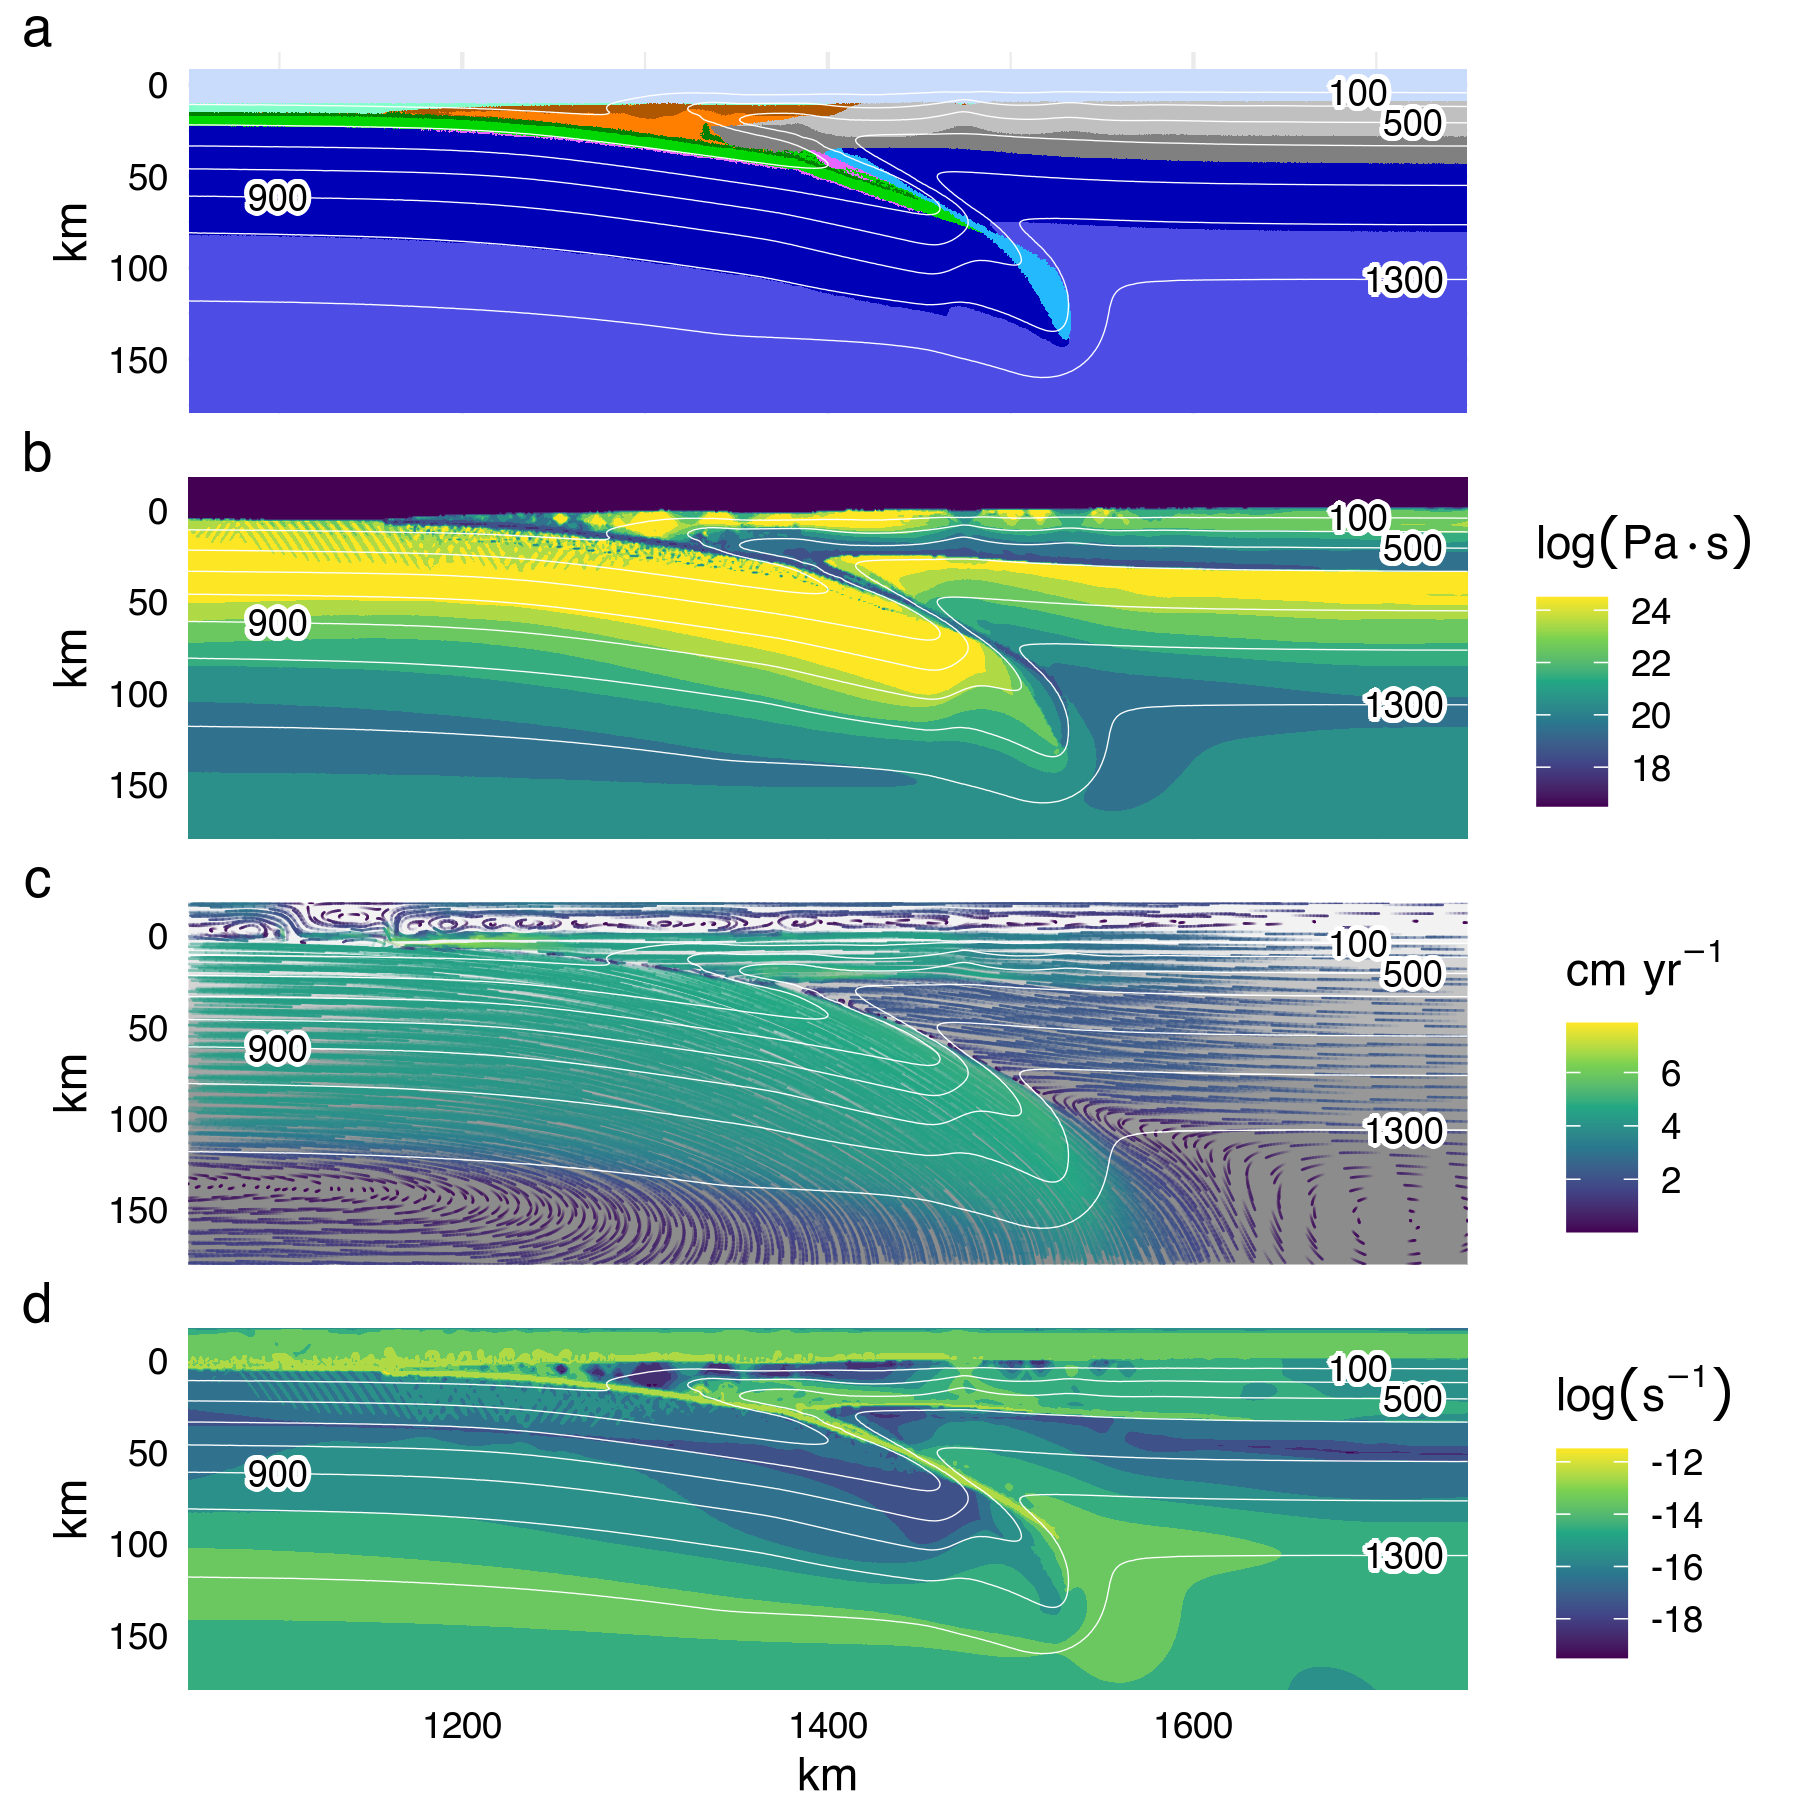
\includegraphics[width=1\linewidth,]{assets/figs/chpt2/figA2} 

}

\caption[Results for model cdf with $Z_{UP}$ = 78 $km$ at 1.64 $Ma$]{Visualizing model cdf with $Z_{UP}$ = 78 $km$ at 1.64 $Ma$. (a) Rock type. (b) Temperature. (c) Viscosity. (d) Streamlines. Early subduction is facilitated by the prescribed initial weak layer cutting the lithosphere. Strain is localized in the weak serpentine layer along the plate interface. The shallow upper-plate mantle is stagnant and loses heat to the subducting plate, promoting serpentine stabiliization to greater depths. Rock type colors are the same as Figure \ref{fig:init}.}\label{fig:cdfStep1}
\end{figure}

\begin{figure}[htbp]

{\centering 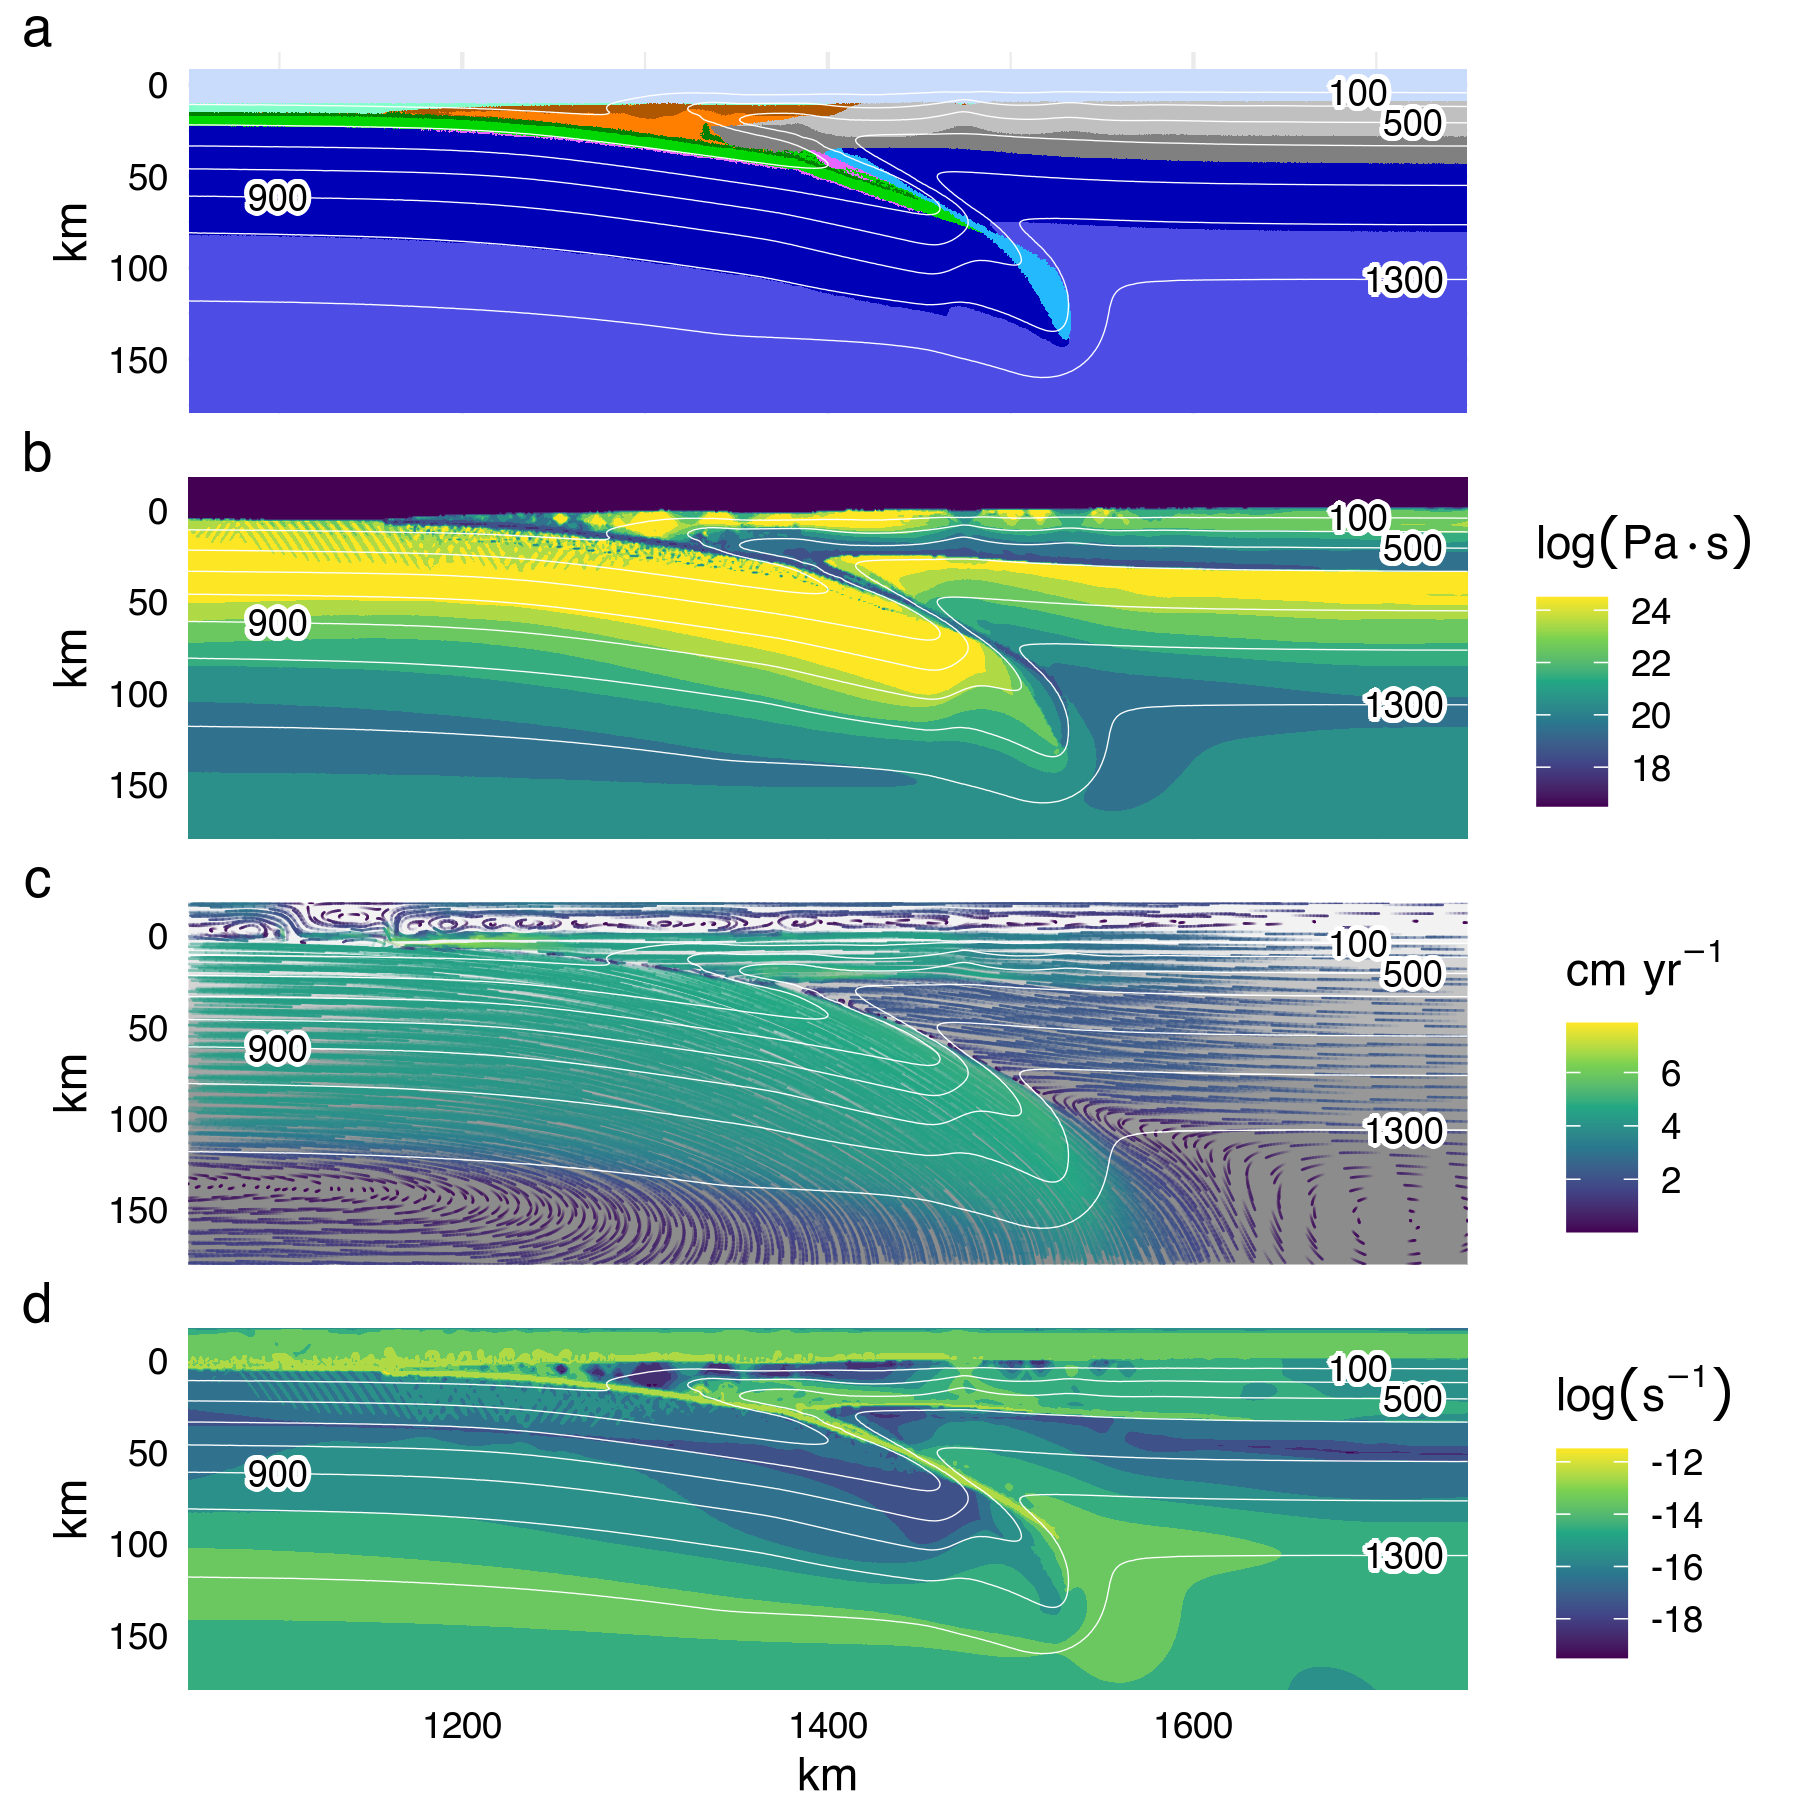
\includegraphics[width=1\linewidth,]{assets/figs/chpt2/figA3} 

}

\caption[Results for model cdf with $Z_{UP}$ = 78 $km$ at 5.05 $Ma$]{Visualizing model cdf with $Z_{UP}$ = 78 $km$ at 5.05 $Ma$. (a) Rock type. (b) Temperature. (c) Viscosity. (d) Streamlines. By 5 $Ma$ balance is achieved between cooling and heating in the shallow and deep upper-plate mantle, respectively. A feedback regulating heat transfer, serpentine destabilization, and mechanical coupling is already stabilizing \gls{cd}. Rock type colors are the same as Figure \ref{fig:init}.}\label{fig:cdfStep2}
\end{figure}

\begin{figure}[htbp]

{\centering 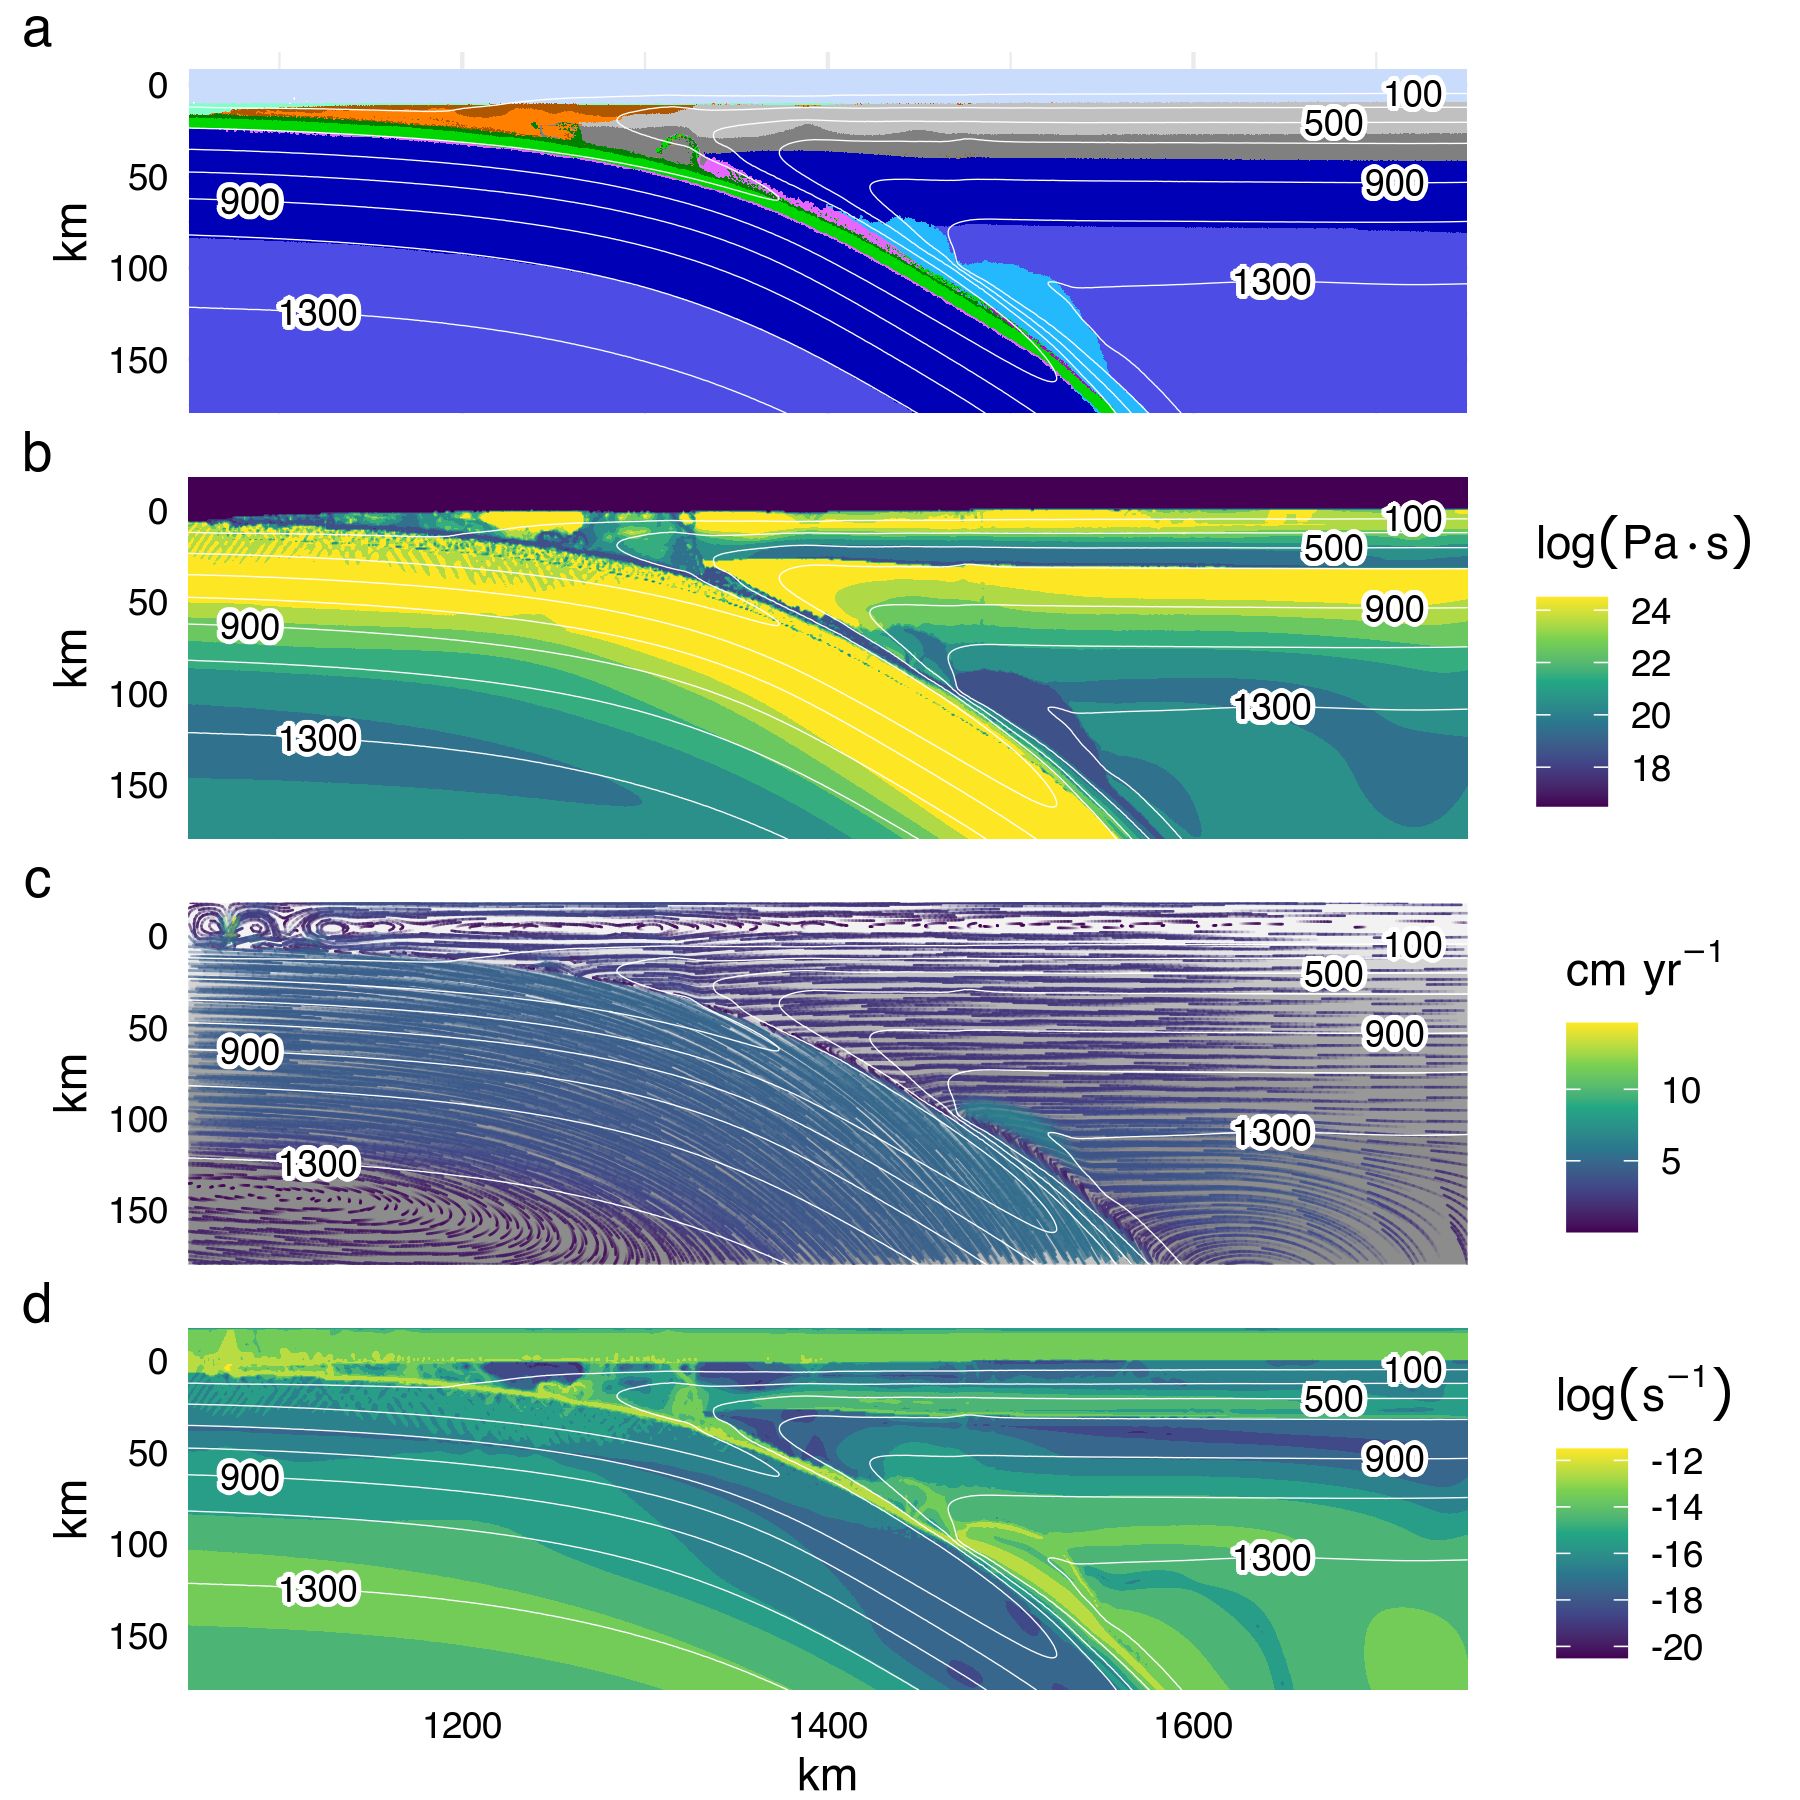
\includegraphics[width=1\linewidth,]{assets/figs/chpt2/figA4} 

}

\caption[Results for model cdf with $Z_{UP}$ = 78 $km$ at 9.93 $Ma$]{Visualizing standard model cdf with $Z_{UP}$ = 78 $km$ at 9.93 $Ma$. (a) Rock type. (b) Temperature. (c) Viscosity. (d) Streamlines. Geodynamics remain approximately constant from 5 $Ma$ (cf. Figure \ref{fig:cdfStep2}). The system remains in steady state for as long water fluxes to the upper-plate mantle and serpentine is stable. Rock type colors are the same as Figure \ref{fig:init}.}\label{fig:cdfStep3}
\end{figure}

\clearpage

\hypertarget{regSummary}{%
\section{Regression summaries}\label{regSummary}}

The form of the preferred quadratic regression model in Section \ref{cdEstimators} (Figure \ref{fig:results} \& Table \ref{tab:zcResults}) implies a lower limit to \gls{cd} of approximately 60 \(km\), even for thin \gls{upt} and, presumably, under warm conditions during nascent subduction. In principle, thin \glspl{upt} could allow effective heat transfer in a flowing shallow asthenospheric mantle---hindering deep stabilization of serpentine. Olivine and pyroxene would be the stable mantle minerals, and strong, shallow coupling between plates would be expected Gerya et al. (\protect\hyperlink{ref-gerya2008}{2008}). However, even the warmest numerical experiments (low-\(\Phi\) \& thin \gls{upt}) in Chapter \ref{chpt2} eventually stabilize serpentine in the shallow upper-plate mantle. This is evident by increasing depth of mechanical coupling with time for the first 5 \(Ma\) of subduction (Figure \ref{fig:antDepth}).

\begin{figure}[htbp]

{\centering 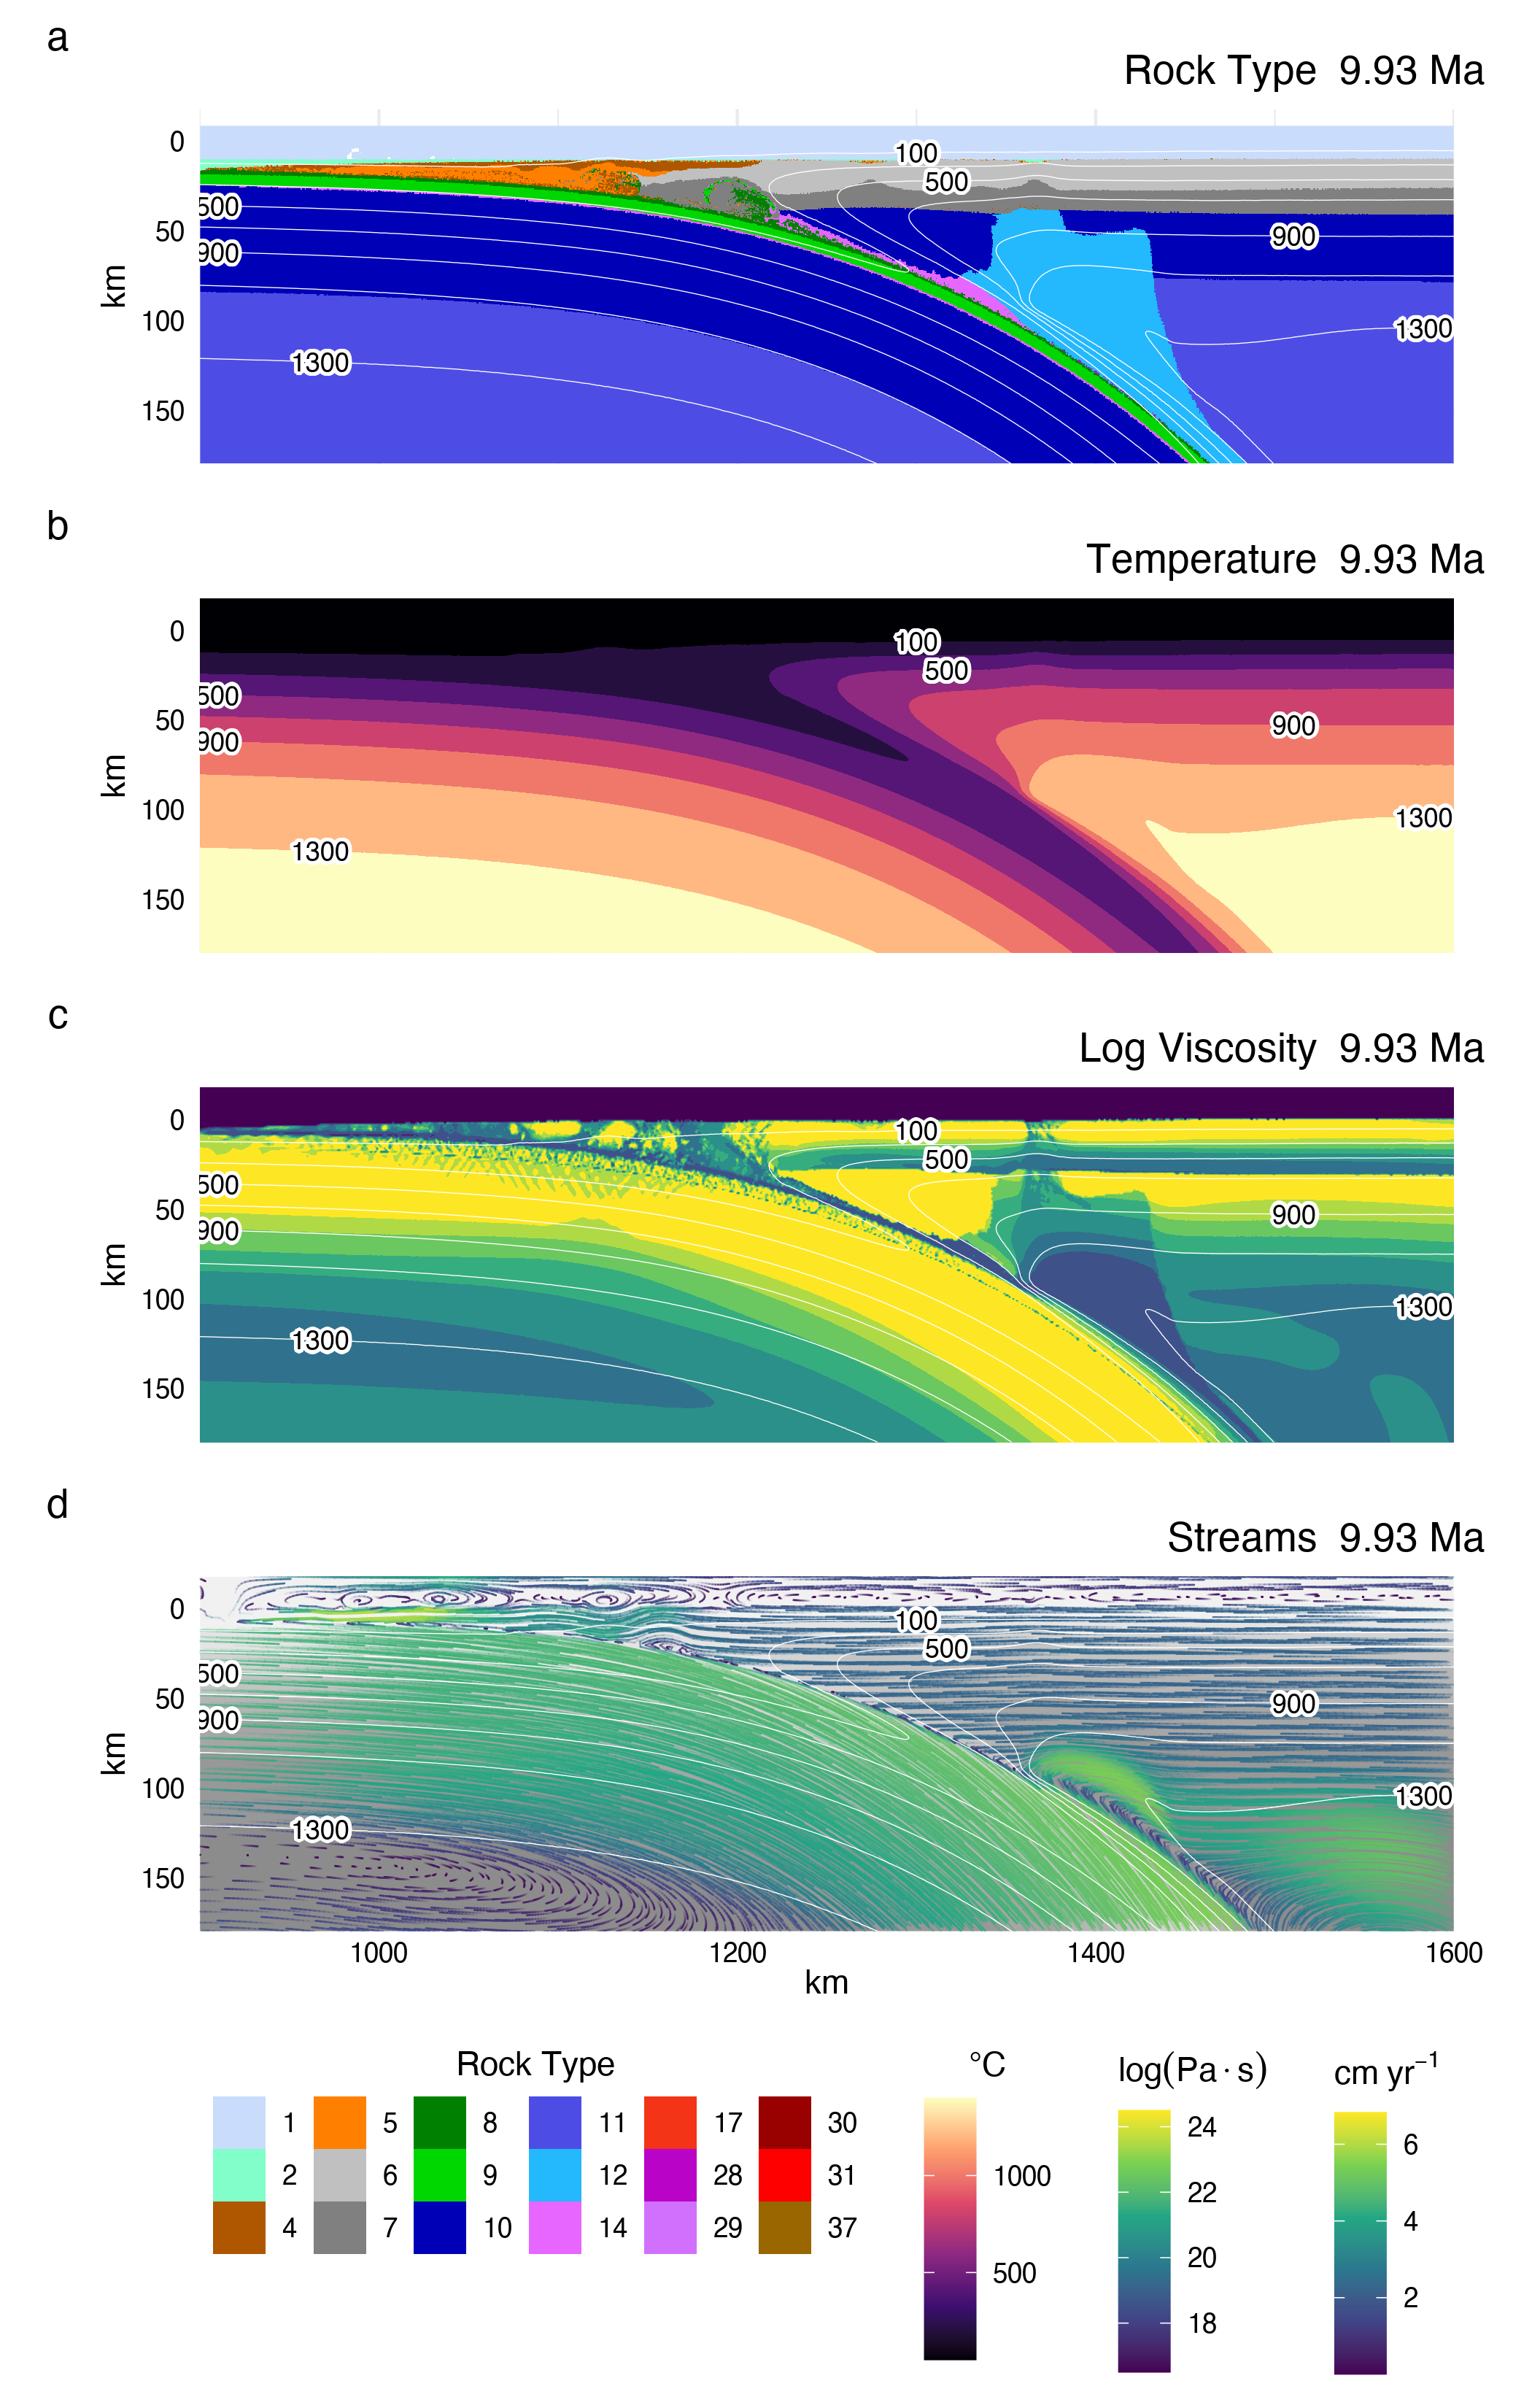
\includegraphics[width=1\linewidth,]{assets/figs/chpt2/figA5} 

}

\caption[Coupling depths determined from numerical experiments]{Coupling depths ($Z_{cpl}$, grayscale) determined from numerical experiments. Model names are listed along the top axis and correspond to the range of thermal parameter $\Phi$ values along the bottom axis. Note that the ($\Phi$) axis is not linear. $Z_{cpl}$ increases systematically with increasing $Z_{UP}$ (change in grayscale down columns) for all models. Trends in $Z_{cpl}$ with respect to $\Phi$ (change in grayscale across rows) are less apparent.}\label{fig:results}
\end{figure}

Summary statistics for the regression models presented in Section \ref{cdEstimators} are given in Tables \ref{tab:anova} and \ref{tab:regSummary}.

\begin{table}
\caption{\label{tab:zcResults}Coupling depth results}

\centering
\begin{tabular}[t]{lrrr}
\toprule
Model & $Z_{UP}$ & $\Phi$ & \vphantom{3} $Z_{cpl}$\\
\midrule
\cellcolor{gray!6}{cda} & \cellcolor{gray!6}{46} & \cellcolor{gray!6}{13.0} & \cellcolor{gray!6}{66}\\
cdb & 46 & 21.5 & 74\\
\cellcolor{gray!6}{cdc} & \cellcolor{gray!6}{46} & \cellcolor{gray!6}{26.1} & \cellcolor{gray!6}{69}\\
cdd & 46 & 32.6 & 67\\
\cellcolor{gray!6}{cde} & \cellcolor{gray!6}{46} & \cellcolor{gray!6}{22.0} & \cellcolor{gray!6}{72}\\
\addlinespace
cdf & 46 & 36.3 & 78\\
\cellcolor{gray!6}{cdg} & \cellcolor{gray!6}{46} & \cellcolor{gray!6}{44.0} & \cellcolor{gray!6}{78}\\
cdh & 46 & 55.0 & 59\\
\cellcolor{gray!6}{cdi} & \cellcolor{gray!6}{46} & \cellcolor{gray!6}{34.0} & \cellcolor{gray!6}{80}\\
cdj & 46 & 56.1 & 70\\
\addlinespace
\cellcolor{gray!6}{cdk} & \cellcolor{gray!6}{46} & \cellcolor{gray!6}{68.0} & \cellcolor{gray!6}{58}\\
cdl & 46 & 85.0 & 65\\
\cellcolor{gray!6}{cdm} & \cellcolor{gray!6}{46} & \cellcolor{gray!6}{44.0} & \cellcolor{gray!6}{79}\\
cdn & 46 & 72.6 & 70\\
\cellcolor{gray!6}{cdo} & \cellcolor{gray!6}{46} & \cellcolor{gray!6}{88.0} & \cellcolor{gray!6}{68}\\
\addlinespace
cdp & 46 & 110.0 & 64\\
\bottomrule
\end{tabular}
\centering
\begin{tabular}[t]{lrrr}
\toprule
\cellcolor{gray!6}{Model} & \cellcolor{gray!6}{$Z_{UP}$} & \cellcolor{gray!6}{$\Phi$} & \cellcolor{gray!6}{\vphantom{2} $Z_{cpl}$}\\
\midrule
cda & 62 & 13.0 & 80\\
\cellcolor{gray!6}{cdb} & \cellcolor{gray!6}{62} & \cellcolor{gray!6}{21.5} & \cellcolor{gray!6}{79}\\
cdc & 62 & 26.1 & 78\\
\cellcolor{gray!6}{cdd} & \cellcolor{gray!6}{62} & \cellcolor{gray!6}{32.6} & \cellcolor{gray!6}{77}\\
cde & 62 & 22.0 & 87\\
\addlinespace
\cellcolor{gray!6}{cdf} & \cellcolor{gray!6}{62} & \cellcolor{gray!6}{36.3} & \cellcolor{gray!6}{82}\\
cdg & 62 & 44.0 & 75\\
\cellcolor{gray!6}{cdh} & \cellcolor{gray!6}{62} & \cellcolor{gray!6}{55.0} & \cellcolor{gray!6}{70}\\
cdi & 62 & 34.0 & 91\\
\cellcolor{gray!6}{cdj} & \cellcolor{gray!6}{62} & \cellcolor{gray!6}{56.1} & \cellcolor{gray!6}{77}\\
\addlinespace
cdk & 62 & 68.0 & 72\\
\cellcolor{gray!6}{cdl} & \cellcolor{gray!6}{62} & \cellcolor{gray!6}{85.0} & \cellcolor{gray!6}{67}\\
cdm & 62 & 44.0 & 88\\
\cellcolor{gray!6}{cdn} & \cellcolor{gray!6}{62} & \cellcolor{gray!6}{72.6} & \cellcolor{gray!6}{77}\\
cdo & 62 & 88.0 & 74\\
\addlinespace
\cellcolor{gray!6}{cdp} & \cellcolor{gray!6}{62} & \cellcolor{gray!6}{110.0} & \cellcolor{gray!6}{75}\\
\bottomrule
\end{tabular}
\centering
\begin{tabular}[t]{lrrr}
\toprule
Model & $Z_{UP}$ & $\Phi$ & \vphantom{1} $Z_{cpl}$\\
\midrule
\cellcolor{gray!6}{cda} & \cellcolor{gray!6}{78} & \cellcolor{gray!6}{13.0} & \cellcolor{gray!6}{87}\\
cdb & 78 & 21.5 & 94\\
\cellcolor{gray!6}{cdc} & \cellcolor{gray!6}{78} & \cellcolor{gray!6}{26.1} & \cellcolor{gray!6}{97}\\
cdd & 78 & 32.6 & 97\\
\cellcolor{gray!6}{cde} & \cellcolor{gray!6}{78} & \cellcolor{gray!6}{22.0} & \cellcolor{gray!6}{90}\\
\addlinespace
cdf & 78 & 36.3 & 90\\
\cellcolor{gray!6}{cdg} & \cellcolor{gray!6}{78} & \cellcolor{gray!6}{44.0} & \cellcolor{gray!6}{88}\\
cdh & 78 & 55.0 & 85\\
\cellcolor{gray!6}{cdi} & \cellcolor{gray!6}{78} & \cellcolor{gray!6}{34.0} & \cellcolor{gray!6}{97}\\
cdj & 78 & 56.1 & 91\\
\addlinespace
\cellcolor{gray!6}{cdk} & \cellcolor{gray!6}{78} & \cellcolor{gray!6}{68.0} & \cellcolor{gray!6}{84}\\
cdl & 78 & 85.0 & 77\\
\cellcolor{gray!6}{cdm} & \cellcolor{gray!6}{78} & \cellcolor{gray!6}{44.0} & \cellcolor{gray!6}{78}\\
cdn & 78 & 72.6 & 87\\
\cellcolor{gray!6}{cdo} & \cellcolor{gray!6}{78} & \cellcolor{gray!6}{88.0} & \cellcolor{gray!6}{85}\\
\addlinespace
cdp & 78 & 110.0 & 78\\
\bottomrule
\end{tabular}
\centering
\begin{tabular}[t]{lrrr}
\toprule
\cellcolor{gray!6}{Model} & \cellcolor{gray!6}{$Z_{UP}$} & \cellcolor{gray!6}{$\Phi$} & \cellcolor{gray!6}{$Z_{cpl}$}\\
\midrule
cda & 94 & 13.0 & 95\\
\cellcolor{gray!6}{cdb} & \cellcolor{gray!6}{94} & \cellcolor{gray!6}{21.5} & \cellcolor{gray!6}{101}\\
cdc & 94 & 26.1 & 108\\
\cellcolor{gray!6}{cdd} & \cellcolor{gray!6}{94} & \cellcolor{gray!6}{32.6} & \cellcolor{gray!6}{113}\\
cde & 94 & 22.0 & 100\\
\addlinespace
\cellcolor{gray!6}{cdf} & \cellcolor{gray!6}{94} & \cellcolor{gray!6}{36.3} & \cellcolor{gray!6}{104}\\
cdg & 94 & 44.0 & 104\\
\cellcolor{gray!6}{cdh} & \cellcolor{gray!6}{94} & \cellcolor{gray!6}{55.0} & \cellcolor{gray!6}{104}\\
cdi & 94 & 34.0 & 101\\
\cellcolor{gray!6}{cdj} & \cellcolor{gray!6}{94} & \cellcolor{gray!6}{56.1} & \cellcolor{gray!6}{102}\\
\addlinespace
cdk & 94 & 68.0 & 101\\
\cellcolor{gray!6}{cdl} & \cellcolor{gray!6}{94} & \cellcolor{gray!6}{85.0} & \cellcolor{gray!6}{107}\\
cdm & 94 & 44.0 & 106\\
\cellcolor{gray!6}{cdn} & \cellcolor{gray!6}{94} & \cellcolor{gray!6}{72.6} & \cellcolor{gray!6}{102}\\
cdo & 94 & 88.0 & 98\\
\addlinespace
\cellcolor{gray!6}{cdp} & \cellcolor{gray!6}{94} & \cellcolor{gray!6}{110.0} & \cellcolor{gray!6}{108}\\
\bottomrule
\end{tabular}
\end{table}

\begin{table}

\caption{\label{tab:anova}Summary of ANOVA test}
\centering
\begin{threeparttable}
\begin{tabular}[t]{lrrrl}
\toprule
\multicolumn{1}{c}{$Z_{UP}$ Groups} & \multicolumn{1}{c}{$Z_{cpl}$ Estimate} & \multicolumn{1}{c}{Upper Bound} & \multicolumn{1}{c}{Lower Bound} & \multicolumn{1}{c}{p value} \\
\multicolumn{1}{c}{} & \multicolumn{1}{c}{$[km]$} & \multicolumn{1}{c}{$[km]$} & \multicolumn{1}{c}{$[km]$} & \multicolumn{1}{c}{}\\
\midrule
\cellcolor{gray!6}{62-46} & \cellcolor{gray!6}{8.3} & \cellcolor{gray!6}{2.5} & \cellcolor{gray!6}{14.0} & \cellcolor{gray!6}{1.84e-03}\\
78-46 & 18.0 & 12.3 & 23.7 & 1.08e-10\\
\cellcolor{gray!6}{94-46} & \cellcolor{gray!6}{33.6} & \cellcolor{gray!6}{27.8} & \cellcolor{gray!6}{39.3} & \cellcolor{gray!6}{1.99e-11}\\
78-62 & 9.8 & 4.0 & 15.5 & 1.83e-04\\
\cellcolor{gray!6}{94-62} & \cellcolor{gray!6}{25.3} & \cellcolor{gray!6}{19.6} & \cellcolor{gray!6}{31.0} & \cellcolor{gray!6}{1.99e-11}\\
\addlinespace
94-78 & 15.6 & 9.8 & 21.3 & 7.31e-09\\
\bottomrule
\end{tabular}
\begin{tablenotes}
\item Pair-wise Tukey's test comparing means between groups. Estimates are differences between means. Null hypothesis is that means are not different
\end{tablenotes}
\end{threeparttable}
\end{table}

\begin{table}

\caption{\label{tab:regSummary}Summary of regression models}
\centering
\begin{threeparttable}
\begin{tabular}[t]{llrrl}
\toprule
Model & Term & Estimate & Std. Error & p value\\
\midrule
\cellcolor{gray!6}{1} & \cellcolor{gray!6}{Intercept} & \cellcolor{gray!6}{89.4} & \cellcolor{gray!6}{3.7} & \cellcolor{gray!6}{2.24e-33}\\
1 & $\phi$ & -0.1 & 0.1 & 1.55e-01\\
\cellcolor{gray!6}{2} & \cellcolor{gray!6}{Intercept} & \cellcolor{gray!6}{36.4} & \cellcolor{gray!6}{3.2} & \cellcolor{gray!6}{7.15e-17}\\
2 & $Z_{UP}$ & 0.7 & 0.0 & 3.73e-23\\
\cellcolor{gray!6}{3} & \cellcolor{gray!6}{Intercept} & \cellcolor{gray!6}{58.9} & \cellcolor{gray!6}{1.7} & \cellcolor{gray!6}{1.43e-41}\\
\addlinespace
3 & $Z_{UP}^2$ & 0.0 & 0.0 & 2.98e-24\\
\cellcolor{gray!6}{4} & \cellcolor{gray!6}{Intercept} & \cellcolor{gray!6}{69.2} & \cellcolor{gray!6}{14.0} & \cellcolor{gray!6}{6.25e-06}\\
4 & $Z_{UP}$ & -0.3 & 0.4 & 4.63e-01\\
\cellcolor{gray!6}{4} & \cellcolor{gray!6}{$Z_{UP}^2$} & \cellcolor{gray!6}{0.0} & \cellcolor{gray!6}{0.0} & \cellcolor{gray!6}{1.95e-02}\\
5 & Intercept & 41.1 & 3.3 & 1.14e-18\\
\addlinespace
\cellcolor{gray!6}{5} & \cellcolor{gray!6}{$Z_{UP}$} & \cellcolor{gray!6}{0.7} & \cellcolor{gray!6}{0.0} & \cellcolor{gray!6}{1.12e-24}\\
5 & $\phi$ & -0.1 & 0.0 & 1.18e-03\\
\cellcolor{gray!6}{6} & \cellcolor{gray!6}{Intercept} & \cellcolor{gray!6}{63.6} & \cellcolor{gray!6}{2.1} & \cellcolor{gray!6}{8.29e-39}\\
6 & $Z_{UP}^2$ & 0.0 & 0.0 & 5.68e-26\\
\cellcolor{gray!6}{6} & \cellcolor{gray!6}{$\phi$} & \cellcolor{gray!6}{-0.1} & \cellcolor{gray!6}{0.0} & \cellcolor{gray!6}{6.98e-04}\\
\addlinespace
7 & Intercept & 73.8 & 12.9 & 3.39e-07\\
\cellcolor{gray!6}{7} & \cellcolor{gray!6}{$Z_{UP}$} & \cellcolor{gray!6}{-0.3} & \cellcolor{gray!6}{0.4} & \cellcolor{gray!6}{4.23e-01}\\
7 & $Z_{UP}^2$ & 0.0 & 0.0 & 1.12e-02\\
\cellcolor{gray!6}{7} & \cellcolor{gray!6}{$\phi$} & \cellcolor{gray!6}{-0.1} & \cellcolor{gray!6}{0.0} & \cellcolor{gray!6}{7.28e-04}\\
\bottomrule
\end{tabular}
\begin{tablenotes}
\item \uline{\textit{models}}: 1: $[z_c=\phi]$, 2: $[z_c=Z_{UP}]$, 3: $[z_c=Z_{UP}^2]$, 4: $[z_c=Z_{UP}+Z_{UP}^2]$, 5: $[z_c=Z_{UP}+\phi]$, 6: [$z_c=Z_{UP}^2+\phi]$, 7: $[z_c=Z_{UP}+Z_{UP}^2+\phi]$
\end{tablenotes}
\end{threeparttable}
\end{table}

\begin{figure}[htbp]

{\centering 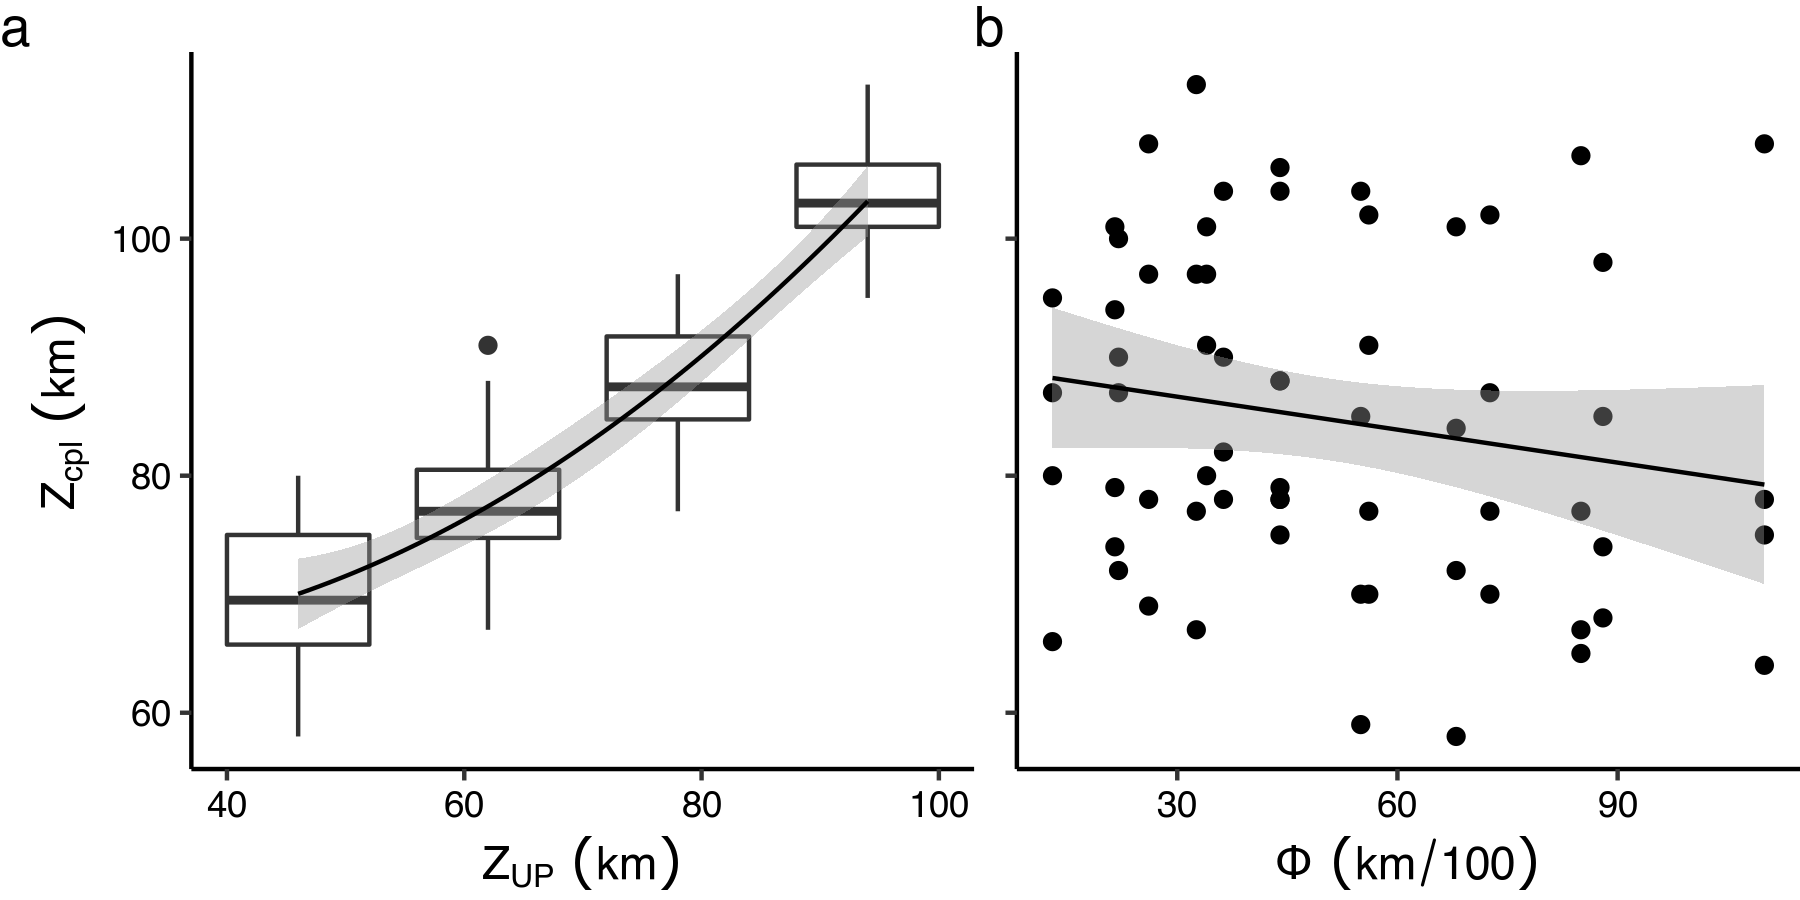
\includegraphics[width=1\linewidth,]{assets/figs/chpt2/figA6} 

}

\caption[Bivariate regressions of coupling results]{Bivariate regressions. (a) Coupling depth ($Z_{cpl}$) vs. upper-plate thickness ($Z_{UP}$) shows $Z_{cpl}$ increasing approximately quadratically with increasing $Z_{UP}$. The correlation is highly significant (see Tables \ref{tab:anova} and \ref{tab:regSummary}) and explains more than 80\% of the variance in $Z_{cpl}$. $Z_{UP}$ alone estimates $Z_{cpl}$ well. (b) $Z_{cpl}$ vs. thermal parameter ($\Phi$) shows no significant correlation (no line fits with a slope significantly different from zero). $\Phi$ has little effect on $Z_{cpl}$ and cannot be used as a standalone estimator.}\label{fig:biv}
\end{figure}

\clearpage

\hypertarget{deHydration}{%
\section{(De)hydration model}\label{deHydration}}

The material properties used in our experiments are listed in Table \ref{tab:materials} and Table \ref{tab:melts}. For details about the sedimentation and erosion, melting and extraction, and rheological models, please refer to Sizova et al. (\protect\hyperlink{ref-sizova2010}{2010}). Here we discuss only the hydrodynamic model, because it is the most relevant aspect of our results.

The hydrodynamics in our models controls the timing and magnitude of mantle wedge hydration. The main sources of water delivered to the mantle are altered basaltic crust and seafloor sediments, which we assumed to contain up to 5 \(wt.\% H_{2}O\). We assumed a gradual expulsion of water from pore space and through quasi-continuous dehydration reactions occurring within the slab. Water content is computed using the following equation:

\begin{equation}
  \chi_{H_{2}O} = \chi_{H_{2}O_{init}}\times\left(1-\frac{\Delta z}{150\times 10^{3}}\right)
\end{equation}

where \(\chi_{H_{2}O_{init}}\) = 5 \(wt.\%\) and \(\Delta z\) is a marker's depth below the topographical surface.

If a rock marker dehydrates, an independent water particle is instantaneously generated at the same location with the respective \(H_{2}O\) content. The new water particle is moved in accordance to the local velocity field, described by the following equation:

\begin{equation}
  \begin{aligned}
    \vec{v}_{\text{water}} & = (\vec{v}_x,\ \vec{v}_z) \\
    \vec{v}_z & = \vec{v}_z - \vec{v}_{z(\text{percolation})} \\
  \end{aligned}
\end{equation}

where \(\vec{v}_{water}\) is the velocity vector of the water particle, \(\vec{v}_{x}\) and \(\vec{v}_{z}\) are the local velocity vectors of the solid state mantle or crust, and \(\vec{v}_{z(percolation)}\) is a imposed constant upward percolation velocity (10 \(cm/year\)). We implicitly neglect kinetics of reactions, as material properties of markers change instantaneously at equilibrium reactions.

\begin{table}

\caption{\label{tab:melts}Melting curves used in numerical experiments}
\centering
\resizebox{\linewidth}{!}{
\begin{threeparttable}
\begin{tabular}[t]{lrrlrlrllrr}
\toprule
Material & a & b & c & d & e & f & g & h & i & j\\
\midrule
\cellcolor{gray!6}{sediments} & \cellcolor{gray!6}{1200} & \cellcolor{gray!6}{889} & \cellcolor{gray!6}{1.79e+04} & \cellcolor{gray!6}{54} & \cellcolor{gray!6}{2.02e+04} & \cellcolor{gray!6}{831} & \cellcolor{gray!6}{6.00e-02} & \cellcolor{gray!6}{} & \cellcolor{gray!6}{1262} & \cellcolor{gray!6}{0.009}\\
felsic crust & 1200 & 889 & 1.79e+04 & 54 & 2.02e+04 & 831 & 6.00e-02 &  & 1262 & 0.009\\
\cellcolor{gray!6}{basalt} & \cellcolor{gray!6}{1600} & \cellcolor{gray!6}{973} & \cellcolor{gray!6}{7.04e+05} & \cellcolor{gray!6}{354} & \cellcolor{gray!6}{7.78e+07} & \cellcolor{gray!6}{935} & \cellcolor{gray!6}{3.50e-03} & \cellcolor{gray!6}{6.2e-05} & \cellcolor{gray!6}{1423} & \cellcolor{gray!6}{0.105}\\
gabbro & 1600 & 973 & 7.04e+05 & 354 & 7.78e+07 & 935 & 3.50e-03 & 6.2e-05 & 1423 & 0.105\\
\cellcolor{gray!6}{mantle dry} & \cellcolor{gray!6}{} & \cellcolor{gray!6}{} & \cellcolor{gray!6}{} & \cellcolor{gray!6}{} & \cellcolor{gray!6}{} & \cellcolor{gray!6}{1394} & \cellcolor{gray!6}{1.33e-01} & \cellcolor{gray!6}{-5.1e-05} & \cellcolor{gray!6}{2073} & \cellcolor{gray!6}{0.114}\\
\addlinespace
mantle hydrated & 2400 & 1240 & 4.98e+04 & 323 &  &  & 1.27e+05 & 3.5e-05 & 2073 & 0.114\\
\cellcolor{gray!6}{serpentine} & \cellcolor{gray!6}{2400} & \cellcolor{gray!6}{1240} & \cellcolor{gray!6}{4.98e+04} & \cellcolor{gray!6}{323} & \cellcolor{gray!6}{} & \cellcolor{gray!6}{} & \cellcolor{gray!6}{1.27e+05} & \cellcolor{gray!6}{3.5e-05} & \cellcolor{gray!6}{2073} & \cellcolor{gray!6}{0.114}\\
\bottomrule
\end{tabular}
\begin{tablenotes}
\item \uline{\textit{solidus curve}}: $T(P)=[b+\frac{c}{(P+d)}+\frac{e}{(P+d)^2}]$ at $P<a$ and $[f+gP+hP^2]$ at $P\geq a$
\item \uline{\textit{liquidus curve}}: $T(P) = i+jP$ with $T$ in $[K]$ and $P$ in $[MPa]$
\item \uline{\textit{reference}}: Schmidt \& Poli (1998)
\end{tablenotes}
\end{threeparttable}}
\end{table}

\hypertarget{rheologicSensitivity}{%
\section{Rheologic sensitivity tests on plate coupling}\label{rheologicSensitivity}}

Numerical modelling practitioners simulating \glspl{sz} approach mechanical coupling between plates differently. A simple, but highly effective approach, is prescribing a layer of arbitrary strength extending from the surface to an arbitrary depth or temperature along the plate interface. This approach effectively inhibits transfer of shear stress between plates and is analogous to controlling a no-slip condition at the interface (plates move with the same velocity vector beyond the coupling point). Numerous models use this method (e.g., \protect\hyperlink{ref-peacock1996}{Peacock, 1996}; \protect\hyperlink{ref-peacock1999b}{Peacock \& Wang, 1999}; \protect\hyperlink{ref-syracuse2010}{Syracuse et al., 2010}; \protect\hyperlink{ref-wada2009}{Wada \& Wang, 2009}) in part because it allows fine-tuning to specific \gls{sz} configurations. Serpentine-or talc-rich horizons are typically invoked to justify implementing such a condition at shallow interface depths.

The experiments outlined in Section \ref{numMethods} do not explicitly define coupling, but rather use a rheologic model that explicitly follows experimentally determined flow laws and mineral stability fields. This approach conceptually follows and extends petrologic explanations for a weak interface (\protect\hyperlink{ref-hyndman2003}{Hyndman \& Peacock, 2003}; \protect\hyperlink{ref-peacock1999a}{Peacock \& Hyndman, 1999}). As a corollary, dehydration of serpentine, or possibly talc, at higher temperatures must strengthen the interface (\protect\hyperlink{ref-agard2016}{Agard et al., 2016}). Noting that talc is unstable at P \(>\) 2.0 \(GPa\) in an ultramafic rock (\protect\hyperlink{ref-schmidt1998}{Schmidt \& Poli, 1998}), a serpentine rheology is arguably the most relevant candidate responsible for a strength increase, and thus coupling, at \gls{pt} conditions inferred for coupling in active \glspl{sz} (\protect\hyperlink{ref-syracuse2010}{Syracuse et al., 2010}; \protect\hyperlink{ref-wada2009}{Wada \& Wang, 2009}).

Sensitivity tests of the rheologic model presented in Section \ref{rheologicModel} were run using diverse experiments adjusting the rheology of serpentine (compared to Table \ref{tab:materials}), the shape and position of the antigorite-out reaction (compared to \eqref{eq:antstab}), and certain hydrodynamic parameters. For brevity, these results are not presented here. The experiments included:

\begin{enumerate}
\def\labelenumi{\arabic{enumi}.}
\tightlist
\item
  antigorite \(\leftarrow\) wet olivine flow law
\item
  antigorite and wet olivine \(\leftarrow\) dry olivine flow law
\item
  isothermal antigorite reaction at 690 \(^{\circ}C\)
\item
  antigorite reaction isothermal Clapeyron slope at 715 \(^{\circ}C\)
\item
  antigorite reaction with positive linear Clapeyron slope
\item
  linear release of \(H_{2}O\) with depth
\item
  no fluid-induced weakening
\end{enumerate}

Only experiments 5 and 7 listed above were inconsistent with the results presented Section \ref{chpt2Results}. Experiment 5 results in transient \glspl{cd} and discontinuous antigorite stability in the upper-plate mantle, whereas experiment 7 results in two-sided subduction (e.g., \protect\hyperlink{ref-gerya2008}{Gerya et al., 2008}). These sensitivity experiments imply numerical coupling mechanisms are mostly contingent on fluid flux to the upper-plate mantle and the implementation of serpentine stability. The experiments also show coupling is relatively insensitive to the exact flow law parameters.

\hypertarget{surface-heat-flow-1}{%
\section{Surface heat flow}\label{surface-heat-flow-1}}

Below is \gls{shf} calculated at 2 \(km\) beneath the topographic surface at approximately 10 \(Ma\) for all numerical experiments presented in Chapter \ref{chpt2}.

\begin{figure}[htbp]

{\centering 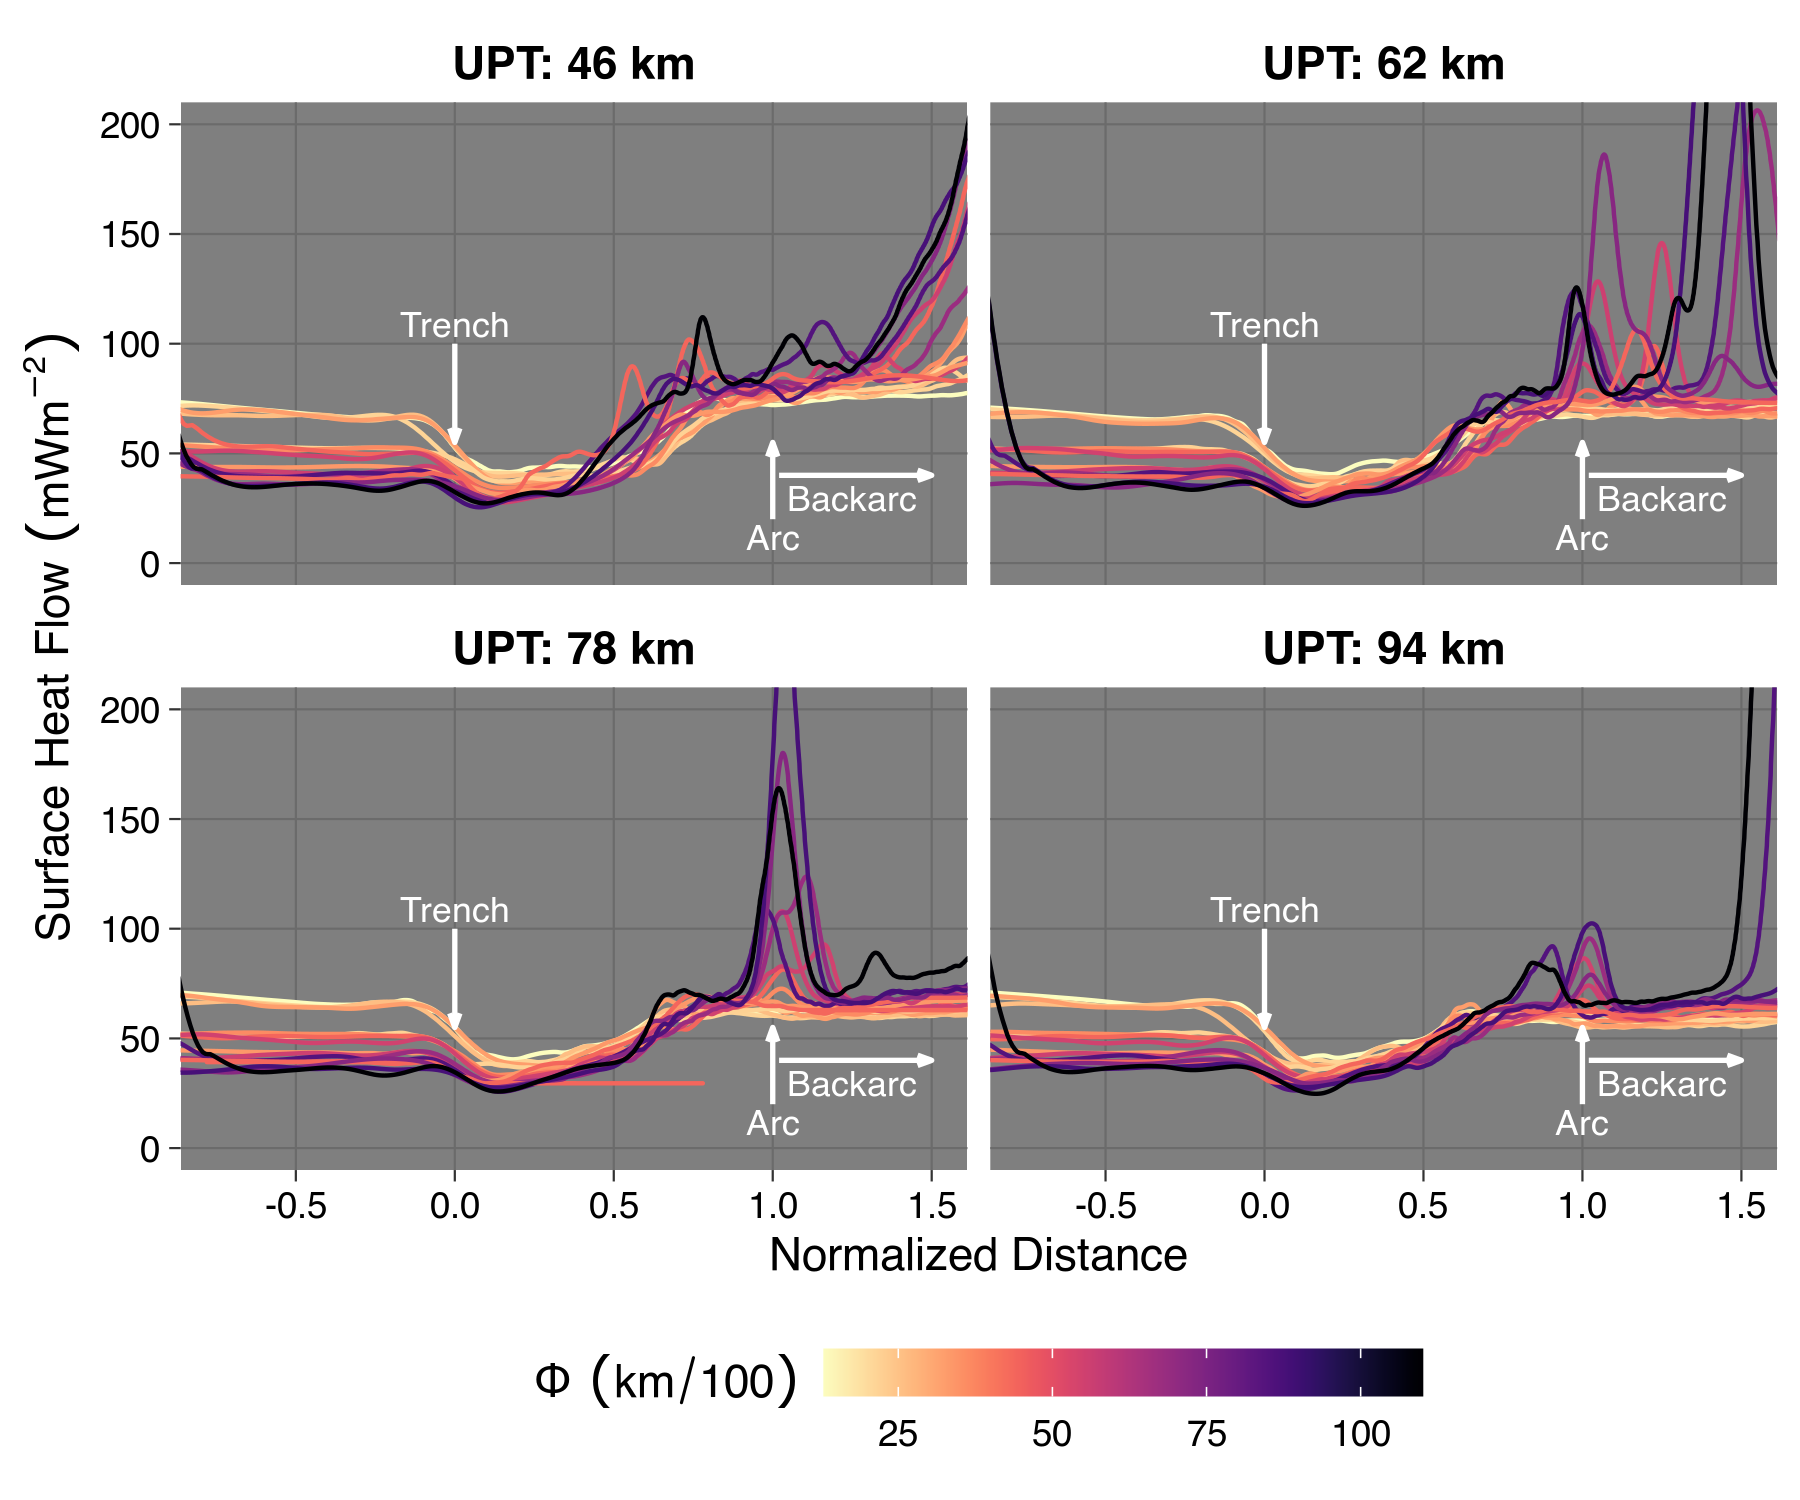
\includegraphics[width=1\linewidth,]{assets/figs/chpt2/figA7} 

}

\caption[Surface heat flow for all numerical experiments]{Surface heat flow calculated at approximately 10 $Ma$ for all numerical experiments. Normalized distance is the distance from the left boundary to the trench, divided by the distance between the trench and arc. Grayscale corresponds to $\Phi$. High amplitude fluctuations near the arc region (normalized distance = 1.0) correspond to vertical migration of fluids and melts. In the backarc region (normalized distance $\geq$ 1.0), these fluctuations correspond to lithospheric extension. Backarc extension is most apparent for high-$\Phi$ experiments (lighter gray lines). Experiments with no extension show a tight distribution of \gls{shf} in the backarc region (darker gray lines).}\label{fig:hf}
\end{figure}

\hypertarget{section}{%
\chapter{}\label{section}}

% Bibliography
\renewcommand\bibname{REFERENCES}
\phantomsection
\cleardoublepage
\addcontentsline{toc}{chapter}{References}
\bibliography{assets/bib/combined.bib}
\markboth{References}{References}

\end{document}
